%%%%%%%%%%%%%%%%%%%%%%%%%%%%%%%%%%%%%%%%%%%%%%%%%%%%%
%            TEMPLATE DE TCC / MONOGRAFIA UESC      %
%       Adequação ao modelo PPGMC/UESC (v5.0)       %
%     Autor: Gabriel Marques de Andrade (2026)      %
%%%%%%%%%%%%%%%%%%%%%%%%%%%%%%%%%%%%%%%%%%%%%%%%%%%%%
\documentclass[oneside]{pacotes/ppgmc-uesc}

% Pacotes adicionais, configurações do siunitx e macros do projeto CubeSat
% ==========================================================================
% macros-cubesat.tex
% Pacotes adicionais, configurações tipográficas e macros do projeto CubeSat
% Compatibilidade: ppgmc-uesc.cls / Overleaf / TeX Live 2023-2026
% ==========================================================================

% Fonte Times New Roman para conformidade ABNT NBR 14724
\usepackage{mathptmx}

% Pacotes para tabelas de alta densidade e tipografia de precisão
\usepackage{booktabs}
\usepackage{tabularx}
\usepackage{siunitx}
\usepackage[protrusion=true,expansion=false]{microtype}

% Configuração do caminho de figuras
\graphicspath{{./04-figuras/}{./figuras/}{./}}

% --------------------------------------------------------------------------
% Configuração do siunitx (ABNT: vírgula decimal e notação científica)
% --------------------------------------------------------------------------
\sisetup{
  output-decimal-marker = {,},
  group-separator       = {.},
  group-minimum-digits  = 4,
  per-mode              = symbol,
  range-phrase          = {~a~},
  range-units           = repeat,
  exponent-product      = \times,
}

% Unidades aeroespaciais e dinâmicas customizadas
\DeclareSIUnit\Grms{\ensuremath{\mathrm{G_{rms}}}}
\DeclareSIUnit\gacc{\ensuremath{\mathrm{g}}}
\DeclareSIUnit\gravity{\ensuremath{\mathrm{G}}}
\DeclareSIUnit\Gacc{\ensuremath{\mathrm{G}}}
\DeclareSIUnit\octave{oitava}
\DeclareSIUnit\torr{Torr}

% --------------------------------------------------------------------------
% Macros de domínio e computacionais
% --------------------------------------------------------------------------
\newcommand{\code}[1]{\texttt{\detokenize{#1}}}
\newcommand{\pendente}[1]{\textbf{\textcolor{red!80!black}{[PENDENTE: #1]}}}
\newcommand{\ph}[1]{\textcolor{red!60!black}{\textit{[#1]}}}
\newcommand{\rail}{\num{8.5}\,$\times$\,\num{8.5}~\si{\milli\metre}}
\newcommand{\figplaceholder}{\fbox{\rule{0pt}{5cm}\rule{0.8\textwidth}{0pt}}}
\newcommand{\Grmsbase}{G_{\text{rms, base}}}
\newcommand{\Grmspay}{G_{\text{rms, payload}}}

% Redefinição robusta de notas para evitar estouro de margem tabular
\renewcommand{\nota}[1]{%
  \par\vspace{0.2cm}%
  \noindent{\footnotesize\textbf{Nota:} #1\par}%
}

% --------------------------------------------------------------------------
% Calibração de profundidade de numeração e Sumário (ABNT NBR 6024)
% Garante hierarquia canônica até subsubseção (nível 4) sem índices quebrados
% --------------------------------------------------------------------------
\setcounter{secnumdepth}{3}
\settocdepth{subsubsection}
\setcounter{tocdepth}{3}
\sloppy


% Informações de autoria, instituição, título e orientação
% ==========================================================================
% 1-Inf.Capa-FolhaRosto.tex
% Informações institucionais, autoria, título e comissão examinadora
% ==========================================================================

% DADOS DA INSTITUIÇÃO
% --------------------------------------------------------------------------
\instituicao{%
  UNIVERSIDADE ESTADUAL DE SANTA CRUZ -- UESC
  \par
  DEPARTAMENTO DE CIÊNCIAS EXATAS E TECNOLÓGICAS
}
\logoInst{
\includegraphics[width=0.8\textwidth]{./04-figuras/brasaouesc}} % Logo da UESC
\programa{Colegiado do Curso de Engenharia Mecânica}

\local{Ilhéus -- BA}
\data{2026}

% DADOS DO TRABALHO
% --------------------------------------------------------------------------
\titulo{CubeSat em Baixa Órbita: Otimização de Volume e Geometria para Maximização de Desempenho Estrutural e Funcional}
\titleenglish{Low Earth Orbit CubeSat: Volume and Geometry Optimization for Structural and Functional Performance Maximization}
\autor{Gabriel Marques de Andrade}
\tipotrabalho{Trabalho de Conclusão de Curso (Graduação)}
\preambulo{Trabalho de Conclusão de Curso apresentado ao Colegiado do Curso de Engenharia Mecânica da Universidade Estadual de Santa Cruz (UESC), como requisito parcial para a obtenção do título de Bacharel em Engenharia Mecânica.}

% ORIENTAÇÃO DO TRABALHO
% --------------------------------------------------------------------------
\orientador[Orientadora:]{Prof.ª Dr.ª Nila Cecília de Faria Lopes Medeiros}
\instOrientador{UESC}

% DADOS DA DEFESA E BANCA EXAMINADORA
% --------------------------------------------------------------------------
\datadefesa{2026}

\bancamembrointerno{Prof.(a) Dr.(a) Examinador(a) Interno(a)}
\bancainstmembrointerno{UESC}

\bancamembroexterno{Prof.(a) Dr.(a) Examinador(a) Externo(a)}
\bancainstmembroexterno{Instituição Externa}


% ==========================================================================
% INÍCIO DO DOCUMENTO
% ==========================================================================
\begin{document}
\pretextual
\frenchspacing

% Elementos pré-textuais
\imprimircapa                     % Capa institucional
\imprimirfolhaderosto{}           % Folha de rosto
%
% Documento: Folha de aprovação-NÃO PRECISA EDITAR-É GERADA AUTOMATICAMENTE
%
\makeatletter
\begin{folhadeaprovacao}

	\begin{center}
		{\large\normalfont\scshape\textbf\imprimirautor}
	\end{center}

	\vspace*{50pt}

	\begin{center}
		\ABNTEXchapterfont\Large\scshape\imprimirtitulo
		\abntex@ifnotempty{\imprimirsubtitulo}{
			{\ABNTEXchapterfont\Large\scshape{\hspace*{-0.3em}: }}{\ABNTEXchapterfont\large\scshape\imprimirsubtitulo}
		}
	\end{center}

	\vspace*{30pt}

%	\abntex@ifnotempty{\imprimirpreambulo}{
%		\SingleSpacing
%		\begin{tabular}{p{.25\textwidth}p{.13\textwidth}p{.44\textwidth}}
%			& \multicolumn{2}{p{.6\textwidth}}{\small\hyphenpenalty=10000{\imprimirpreambulo}} \\ & & \\
%		\end{tabular}
%	}
%
%	\vspace*{7pt}

	\begin{center}
		\imprimirlocal, \imprimirdatadefesa
		\end{center}
		
		\vspace*{7pt}
		\begin{center}
		Comissão Examinadora
		\end{center}
\vspace{-2pt}
\begin{center}
\begin{tabular}{cc}
	\assinatura{\textbf{\imprimirorientador} \\ UESC\\ (Orientadora)}&\\
	% \assinatura{\textbf{\imprimircoorientador} \\ \imprimirinstCoorientador\\ (Coorientador)}&\\ 
	\assinatura{\textbf{\imprimirbancamembrointerno} \\ \imprimirbancainstmembrointerno} &\\
	\assinatura{\textbf{\imprimirbancamembroexterno} \\ \imprimirbancainstmembroexterno}&\\
	
\end{tabular}
	
	\end{center}
%	\begin{center}
%		\assinatura{\textbf{\imprimirorientador} \\ Orientador} 
%		\assinatura{\textbf{Professor} \\ Convidado 1}
%		\assinatura{\textbf{Professor} \\ Convidado 2}
%		%\assinatura{\textbf{Professor} \\ Convidado 3}
%		%\assinatura{\textbf{Professor} \\ Convidado 4}
%	\end{center}

%	\vspace*{\fill}

%	\begin{center}
%		\normalfont\scshape{\imprimirinstituicao}\\
%		\normalfont\scshape{\imprimirprograma}\\
%		\normalfont\scshape{\imprimirlocal}\\
%		\normalfont\scshape{\imprimirdata}
%	\end{center}

\end{folhadeaprovacao}
%\makeatother
 % Folha de aprovação
%
% Documento: Dedicatória-EDITAR-OPCIONAL
%

\begin{dedicatoria}

Espaço reservado para dedicatória.
Inserir seu texto aqui...

\end{dedicatoria}
    % Dedicatória
%
% Documento: Agradecimentos-OPCIONAL
\pagestyle{empty}

\begin{agradecimentos}
\begin{incisos}
\item Nesta parte o discente tem a oportunidade de agradecer a todas as pessoas que foram relevantes durante o desenvolvimento do trabalho.
\item A ordem em que as pessoas são mencionadas pressupõe a importância que tiveram para a realização do trabalho. Assim, incluem-se aqueles que proporcionaram a oportunidade de trabalho, financiaram a pesquisa, contribuíram cientificamente durante a discussão do trabalho e resolveram problemas experimentais.
\item Você pode incluir o agradecimento ao orientador, coorientador e outras pessoas que contribuíram direta ou indiretamente para a realização do trabalho no primeiro item da lista, como: ``Gostaria de agradecer ao meu orientador, [nome do orientador], e coorientador, [nome do coorientador], pelo suporte, orientação e conhecimento compartilhado durante toda a jornada. Também agradeço as demais pessoas da instituição que contribuíram direta ou indiretamente para a realização deste trabalho. Sem o apoio e incentivo de todos vocês, este trabalho não seria possível''.
\item Aos colegas de trabalho que contribuíram para a convivência harmoniosa no local de trabalho, agradeço pela colaboração e amizade durante todo o processo.
\item os técnicos, secretários e demais colaboradores que contribuíram para a realização do trabalho, meu sincero agradecimento pela dedicação e esforço.
\item 	À minha família e aos membros presentes ou ausentes que apoiaram e incentivaram durante toda a jornada, meu agradecimento por todo amor e suporte emocional.
\item É importante lembrar que o trabalho de conclusão baseia-se em hipóteses, experimentações, resultados e discussões científicas. Portanto, não se deve confundir aspectos religiosos com acadêmicos, mas cada um é livre para exercer seu direito de agradecimento da  forma que achar melhor possível. 
\end{incisos}

\end{agradecimentos}
 % Agradecimentos
%
% Documento: Epígrafe-EDITAR NO AMBIENTE EIPIGRAFE- ELEMENTO OPICIONAL
%

\begin{epigrafe}

\textit{``Aqui fica o seu epígrafe.''}

\end{epigrafe}
       % Epígrafe
% ==========================================================================
% resumoPt.tex
% Resumo em língua vernácula (NBR 6028)
% ==========================================================================

\begin{center}
\ABNTEXchapterfont\bfseries\Large\imprimirtitulo
\end{center}

\begin{resumo}
A democratização do acesso à baixa órbita terrestre por meio de nanossatélites da classe CubeSat impõe desafios rigorosos de engenharia de sistemas. Durante o lançamento e a ejeção, o chassi estrutural é submetido a carregamentos dinâmicos severos, como o choque transiente na interface do \textit{Poly-Picosatellite Orbital Deployer} (P-POD) e a vibração aleatória acústica regulamentada pela norma NASA GSFC-STD-7000A (GEVS). Chassis monolíticos convencionais apresentam elevada massa e transferem altos níveis de aceleração à carga útil devido ao acoplamento dinâmico direto. Este trabalho propõe uma rota computacional de alto desempenho para a concepção, a modelagem paramétrica e a otimização multiobjetivo de um chassi CubeSat 1U com painéis constituídos por metamateriais auxéticos reentrantes em liga aeroespacial AlSi10Mg, fabricado por Fusão em Leito de Pó a Laser (L-PBF). Um modelo paramétrico tridimensional, sujeito a critérios estritos de Manufatura Aditiva (DfAM), foi integrado a rotinas automatizadas de elementos finitos de alta fidelidade em ambiente aberto (Code\_Aster e Gmsh Tet10 em Linux/WSL) para gerar um conjunto de 250 simulações de alta fidelidade (análise modal por bloco de Lanczos e resposta espectral à vibração aleatória). Treinou-se um modelo substituto neural residual guiado por física (\textit{Physics-Guided ResNet}), com função de perda composta pelas leis fenomenológicas de Gibson-Ashby e por um termo de monotonicidade de rigidez, que alcançou $\overline{R^2} = \num{0.9874}$ e latência de inferência de \SI{0.405}{\milli\second} (aceleração superior a \num{200000} vezes). Uma máquina de estados finitos determinística, implementada em LangGraph como grafo de fluxo de dados fortemente tipado, orquestrou o descarte precoce de candidatos inviáveis. A otimização multiobjetivo pelo algoritmo NSGA-II, com \num{10000} avaliações de função, mapeou a fronteira de Pareto entre massa e transmissibilidade. Pelo método multicritério TOPSIS, elegeu-se o projeto ótimo de voo ($\theta = \SI{65.75}{\degree}$, $t = \SI{0.613}{\milli\metre}$, $\nu_{\text{eff}} = \num{-13.81}$). A validação numérica de alta ordem em elementos finitos (\textit{Code\_Aster Ground Truth}) confirmou erro de \SI{0.99}{\percent} na tensão de pico e de \SI{0.008}{\percent} na transmissibilidade. Em relação ao chassi monolítico convencional, a estrutura auxética otimizada proporcionou redução de massa de \SI{62.49}{\percent} (\SI{0.308}{\kilo\gram} $\to$ \SI{0.116}{\kilo\gram}), atenuação elastodinâmica de \SI{76.50}{\percent} na transmissibilidade vibratória (\SI{12.6}{\decibel} por filtragem mecânica e desacoplamento de impedância acústica), frequência fundamental de \SI{579.62}{\hertz} e pleno atendimento aos critérios de escoamento e de fadiga estocástica de Steinberg ($D = \num{0.046} \ll \num{0.25}$), qualificando a tecnologia para operação aeroespacial.

\vspace{\onelineskip}
\noindent
\textbf{Palavras-chave}: CubeSat 1U. Metamateriais auxéticos. \textit{Design for Additive Manufacturing}. Redes neurais guiadas por física. Otimização multiobjetivo NSGA-II. NASA GEVS.
\end{resumo}
       % Resumo em Português
% ==========================================================================
% resumoEn.tex
% Abstract em língua estrangeira (Inglês)
% ==========================================================================

\begin{center}
\ABNTEXchapterfont\bfseries\Large\imprimirtitleenglish
\end{center}

\begin{resumo}[Abstract]
\begin{otherlanguage*}{english}
The democratization of access to Low Earth Orbit (LEO) via CubeSat-class nanosatellites imposes severe systems engineering challenges. During launch and deployment, the primary chassis is subjected to harsh dynamic environments, including transient shock inside the Poly-Picosatellite Orbital Deployer (P-POD) and random acoustic vibration governed by NASA GSFC-STD-7000A (GEVS). Conventional monolithic chassis exhibit high mass and limited dynamic isolation, transferring critical vibration levels directly to sensitive electronic payloads. This work presents a high-performance computational framework for the parametric modeling, physics-guided deep learning acceleration, and multi-objective optimization of a 1U CubeSat chassis featuring re-entrant auxetic metamaterial panels manufactured via Laser Powder Bed Fusion (L-PBF) in aerospace AlSi10Mg alloy. A 3D parametric CAD model incorporating strict Design for Additive Manufacturing (DfAM) gates was coupled with batch Ansys MAPDL finite element simulations (Block Lanczos prestressed modal extraction and random vibration PSD analysis), producing a high-fidelity dataset of 250 design points. A residual deep neural surrogate model (Physics-Guided ResNet) was developed with a composite loss function penalizing deviations from Gibson-Ashby scaling laws and enforcing stiffness monotonicity, achieving an average $R^2$ of $0.9874$ and an inference latency of \SI[output-decimal-marker={.}]{0.405}{\milli\second} (more than \num[group-separator={,}]{200000}$\times$ speedup over FEA). A deterministic state machine built with LangGraph as a strongly typed dataflow graph orchestrated early rejection of non-compliant geometries. Multi-objective evolutionary search via NSGA-II over \num[group-separator={,}]{10000} candidate evaluations mapped the Pareto frontier between structural mass and payload transmissibility. Using the TOPSIS multi-criteria decision method, the optimal flight design was selected ($\theta = \SI[output-decimal-marker={.}]{65.75}{\degree}$, $t = \SI[output-decimal-marker={.}]{0.613}{\milli\metre}$, $\nu_{\text{eff}} = -13.81$). High-order FEA ground truth verification showed close agreement with the neural predictions (\SI[output-decimal-marker={.}]{0.99}{\percent} error in $3\sigma$ peak stress and \SI[output-decimal-marker={.}]{0.008}{\percent} in transmissibility). Compared with the conventional solid aluminum chassis, the optimized auxetic design achieved a mass reduction of \SI[output-decimal-marker={.}]{62.49}{\percent} (\SI[output-decimal-marker={.}]{0.308}{\kilo\gram} $\to$ \SI[output-decimal-marker={.}]{0.116}{\kilo\gram}), passive elastodynamic vibration attenuation of \SI[output-decimal-marker={.}]{76.50}{\percent} (\SI[output-decimal-marker={.}]{12.6}{\decibel} reduction via mechanical wave filtering and acoustic impedance mismatch), a fundamental frequency of \SI[output-decimal-marker={.}]{579.62}{\hertz}, and full compliance with NASA GEVS stress margins and Steinberg random fatigue limits ($D = 0.046 \ll 0.25$), demonstrating flight qualification readiness.

\vspace{\onelineskip}
\noindent
\textbf{Keywords}: 1U CubeSat. Auxetic metamaterials. Design for additive manufacturing. Physics-guided neural networks. NSGA-II multi-objective optimization. NASA GEVS.
\end{otherlanguage*}
\end{resumo}
       % Abstract em Inglês
%
% Documento: Lista de figuras-NÃO EDITAR-GERA AUTOMATICAMENTE
%

\pdfbookmark[0]{\listfigurename}{lof}
\listoffigures*
\cleardoublepage
   % Lista de figuras
%
% Documento: Lista de tabelas-NÃO EDITAR-GERA AUTOMATICAMENTE
%

\pdfbookmark[0]{\listtablename}{lot}
\listoftables*
\cleardoublepage
   % Lista de tabelas
% ==========================================================================
% listaSiglas.tex
% Lista de abreviaturas e siglas
% ==========================================================================

\begin{siglas}
  \item[ABNT] Associação Brasileira de Normas Técnicas
  \item[AEB] Agência Espacial Brasileira
  \item[AlSi10Mg] Liga de Alumínio, Silício e Magnésio para Manufatura Aditiva
  \item[CAD] \textit{Computer-Aided Design} (Projeto Auxiliado por Computador)
  \item[CAE] \textit{Computer-Aided Engineering} (Engenharia Auxiliada por Computador)
  \item[CalPoly] \textit{California Polytechnic State University}
  \item[CDS] \textit{CubeSat Design Specification}
  \item[DfAM] \textit{Design for Additive Manufacturing} (Projeto para Manufatura Aditiva)
  \item[DoE] \textit{Design of Experiments} (Planejamento de Experimentos)
  \item[FDM] \textit{Fused Deposition Modeling} (Modelagem por Fusão e Deposição)
  \item[FEA] \textit{Finite Element Analysis} (Análise por Elementos Finitos)
  \item[FGL] \textit{Functionally Graded Lattice} (Treliça com Gradação Funcional)
  \item[GEVS] \textit{General Environmental Verification Standard} (NASA GSFC-STD-7000A)
  \item[HPC] \textit{High-Performance Computing} (Computação de Alto Desempenho)
  \item[INPE] Instituto Nacional de Pesquisas Espaciais
  \item[ITA] Instituto Tecnológico de Aeronáutica
  \item[LEO] \textit{Low Earth Orbit} (Órbita Baixa Terrestre)
  \item[LHS] \textit{Latin Hypercube Sampling} (Amostragem por Hipercubo Latino)
  \item[L-PBF] \textit{Laser Powder Bed Fusion} (Fusão em Leito de Pó a Laser)
  \item[Tet10] Elemento Tetraédrico Quadrático de 10 Nós (Segunda Ordem)
  \item[WSL] \textit{Windows Subsystem for Linux}
  \item[MCP] \textit{Model Context Protocol}
  \item[NASA] \textit{National Aeronautics and Space Administration}
  \item[NRMSE] \textit{Normalized Root Mean Squared Error} (Erro Quadrático Médio Normalizado)
  \item[NSGA-II] \textit{Non-dominated Sorting Genetic Algorithm II}
  \item[PBC] \textit{Periodic Boundary Conditions} (Condições Periódicas de Contorno)
  \item[PLA] Poliácido Láctico (\textit{Polylactic Acid})
  \item[P-POD] \textit{Poly-Picosatellite Orbital Deployer}
  \item[PSD] \textit{Power Spectral Density} (Densidade Espectral de Potência)
  \item[ResNet] \textit{Residual Neural Network} (Rede Neural Residual)
  \item[RVE] \textit{Representative Volume Element} (Elemento de Volume Representativo)
  \item[SEA] \textit{Specific Energy Absorption} (Absorção Específica de Energia)
  \item[SRS] \textit{Shock Response Spectrum} (Espectro de Resposta ao Choque)
  \item[TOPSIS] \textit{Technique for Order Preference by Similarity to Ideal Solution}
  \item[UESC] Universidade Estadual de Santa Cruz
\end{siglas}
    % Lista de siglas
% ==========================================================================
% listaSimbolos.tex
% Lista de símbolos físicos e matemáticos
% ==========================================================================

\begin{simbolos}
  \item[$\theta$] Ângulo de reentrância da célula unitária auxética
  \item[$t$] Espessura da costela/parede celular
  \item[$l$] Comprimento da costela oblíqua reentrante
  \item[$h$] Altura da costela vertical da célula
  \item[$\rho^* / \rho_s$] Densidade relativa da estrutura celular auxética
  \item[$\nu_{\text{eff}}$] Coeficiente de Poisson efetivo homogeneizado
  \item[$E^*$] Módulo de elasticidade efetivo da estrutura celular
  \item[$E_s$] Módulo de elasticidade do material sólido parente (AlSi10Mg)
  \item[$\sigma_y$] Limite de escoamento do material
  \item[$\sigma_{\text{adm}}$] Tensão admissível de qualificação com fator de segurança
  \item[$\sigma_{3\sigma}$] Tensão de pico equivalente no patamar estocástico de $3\sigma$
  \item[$f_1$] Primeira frequência própria fundamental
  \item[$T$] Coeficiente de transmissibilidade dinâmica passiva
  \item[$G_{\text{rms, base}}$] Aceleração eficaz global na base do veículo lançador (\SI{14.1}{\Grms})
  \item[$G_{\text{rms, payload}}$] Aceleração eficaz transmitida à carga útil
  \item[$D$] Índice de dano cumulativo de fadiga de Steinberg / Palmgren-Miner
  \item[$MS_{\text{yield}}$] Margem de Segurança estrutural em relação ao escoamento
  \item[$MS_{\text{shock}}$] Margem de Segurança estrutural em relação ao choque
  \item[$\zeta$] Razão de amortecimento estrutural crítico (\SI{2.0}{\percent})
  \item[$Q$] Fator de qualidade / amplificação modal dinâmica ($Q = 25$)
  \item[$\mathbf{k}$] Vetor de onda elastodinâmico no espaço recíproco
  \item[$\Gamma, \mathrm{X}, \mathrm{M}$] Pontos de alta simetria da Zona Irredutível de Brillouin
  \item[$C_i^*$] Coeficiente de proximidade relativa à solução ideal positiva (TOPSIS)
  \item[$w_i$] Pesos de ponderação multicritério
\end{simbolos}
  % Lista de símbolos
%
% Documento: Sumário-NÃO EDITAR - O SUMÉRIO É GERADO AUTOMATICAMENTE
%

\pdfbookmark[0]{\contentsname}{toc}
\tableofcontents*
\cleardoublepage        % Sumário

% ==========================================================================
% ELEMENTOS TEXTUAIS
% ==========================================================================
\textual

\chapter{Introdução}
\label{cap:introducao}
% --------------------------------------------------------------------------

A democratização do acesso à órbita baixa terrestre (\textit{Low Earth Orbit} -- LEO), impulsionada pela padronização da arquitetura \textit{CubeSat Design Specification} (CALIFORNIA POLYTECHNIC STATE UNIVERSITY, 2022), viabilizou a execução de experimentos científicos e tecnológicas por universidades e centros de pesquisa a custos substancialmente inferiores aos das missões espaciais tradicionais. No entanto, a padronização de volume e massa inerente a essa classe de nanossatélites, ilustrada pelo arranjo estrutural do nanossatélite universitário brasileiro ITASAT-1 na Figura~\ref{fig:itasat}, impõe severas restrições mecânicas. Durante as etapas de ascensão no veículo lançador e na ejeção orbital, o chassi primário do nanossatélite é submetido a um ambiente mecânico dinâmico severo, governado por normas internacionais rigorosas, como o \textit{General Environmental Verification Standard} (GEVS) (NASA, 2013). As diretrizes da Agência Espacial Brasileira (AEB, 2026) preconizam que a integridade estrutural do satélite e a proteção dos subsistemas de bordo exigem frequências naturais fundamentais elevadas ($f_1 \ge \SI{100.0}{\hertz}$), de modo a prevenir a ocorrência de ressonância com os modos acústicos e de baixa frequência do foguete.

\begin{figure}[htb]
  \caption{Arranjo estrutural e distribuição de subsistemas do nanossatélite universitário ITASAT-1}
  \label{fig:itasat}
  \begin{center}
    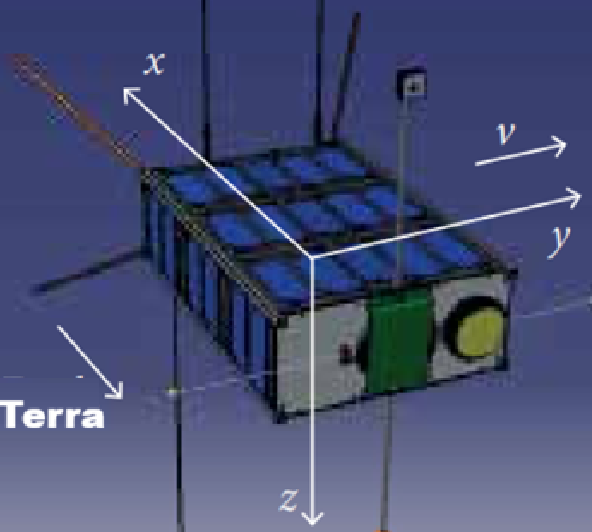
\includegraphics[width=0.75\textwidth]{figuras/itasat1_estrutura.png}
  \end{center}
  \fonte{Adaptado de Carrara \textit{et al.} (2017).}
\end{figure}

Investigações dinâmicas conduzidas em projetos nacionais como o nanossatélite SPORT (SANTOS \textit{et al.}, 2020), desenvolvido conjuntamente pelo Instituto Tecnológico de Aeronáutica (ITA), pelo Instituto Nacional de Pesquisas Espaciais (INPE) e pela NASA, evidenciam que a interface física entre o nanossatélite e o casulo lançador constitui a fonte primária de excitação vibratória e transitória de choque. Concebido com base no padrão operacional do \textit{Poly-Picosatellite Orbital Deployer} (P-POD) (PUIG-SUARI \textit{et al.}, 2002), o mecanismo cinemático de ejeção utiliza a expansão de uma mola principal para impulsionar o satélite ao longo de trilhos de deslizamento, conforme esquematizado na Figura~\ref{fig:interface}. Esse sistema opera sob regime de atrito seco e contato direto metal-metal entre os trilhos do satélite e o interior do tubo lançador. Por exigência normativa estrita da especificação CubeSat, os quatro trilhos longitudinais de \rail{} devem permanecer monolíticos, contínuos e dotados de rugosidade superficial controlada ($Ra \le \SI{1.6}{\micro\metre}$), impedindo qualquer descontinuidade geométrica externa que possa induzir travamento mecânico (\textit{jamming}). Em virtude dessa restrição de contorno fixa, qualquer estratégia de alívio de massa e de isolamento dinâmico passivo deve ser concentrada estritamente nos painéis estruturais internos do chassi.

\begin{figure}[htb]
  \caption{Interface mecânica e cinemática de contato entre os trilhos do CubeSat e o dispensador orbital P-POD durante o curso de ejeção}
  \label{fig:interface}
  \begin{center}
    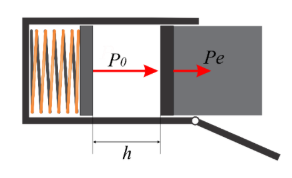
\includegraphics[width=0.65\textwidth]{figuras/interface_cubesat_deployer.png}
  \end{center}
  \fonte{Adaptado de Santos \textit{et al.} (2020).}
\end{figure}

Tradicionalmente, os chassis da classe CubeSat são usinados a partir de blocos maciços de ligas de alumínio aeroespacial, como o Al 6061-T6. Embora apresentem propriedades estáticas consolidadas, tais estruturas contínuas exibem acoplamento dinâmico rígido direto e reduzida capacidade de filtragem mecânica de frequências operacionais, transferindo quase integralmente a densidade espectral de potência (PSD) de vibração aleatória da base para as placas eletrônicas e cargas úteis sensíveis (SLEJKO \textit{et al.}, 2023). Como alternativa a esse gargalo físico, pesquisas recentes na fronteira da mecânica dos sólidos apontam para o uso de metamateriais celulares auxéticos com coeficiente de Poisson negativo ($\nu < 0$) (LI \textit{et al.}, 2026). Geometrias reentrantes, quando submetidas a solicitações mecânicas dinâmicas, exibem rotação controlada de costelas oblíquas e contração lateral sob tração (ou expansão lateral sob compressão), conferindo elevada Absorção Específica de Energia (\textit{Specific Energy Absorption} -- SEA), resiliência a impactos e formação de zonas proibidas de propagação de ondas elásticas (\textit{phononic bandgaps}) por interferência destrutiva e desacoplamento de impedância acústica (CUI \textit{et al.}, 2025; FARSHBAF \textit{et al.}, 2025). Tais propriedades tornam as treliças auxéticas candidatas ideais para atuarem simultaneamente como elemento estrutural resistente e como filtro passa-faixa/passa-baixa elastodinâmico passivo.

A viabilidade de manufatura dessas geometrias celulares complexas decorre do avanço da Manufatura Aditiva por Fusão em Leito de Pó a Laser (\textit{Laser Powder Bed Fusion} -- L-PBF), governada pelos preceitos de \textit{Design for Additive Manufacturing} (DfAM) (KHAN; RICCIO, 2024). Ensaios experimentais prévios demonstraram a aptidão de estruturas de suporte espacial manufaturadas aditivamente para resistir a perfis de qualificação aleatória GEVS sem falha estrutural (ROBERTS, 2018). Todavia, o dimensionamento e a otimização de matrizes celulares com modulação espacial de espessuras impõem barreiras computacionais críticas: a avaliação de uma única geometria por simulação tridimensional de Elementos Finitos (FEA) de alta fidelidade demanda tempos de processamento da ordem de minutos a horas, inviabilizando varreduras evolutivas com milhares de indivíduos. Para transpor esse custo proibitivo com rigor físico estrito, torna-se imprescindível a incorporação de Modelos Substitutos Neurais Guiados por Física (\textit{Physics-Guided Machine Learning}), fundamentados nas leis fenomenológicas de escala de Gibson e Ashby (1997), e orquestrados por uma máquina de estados finitos determinística em grafo de fluxo fortemente tipado (LangGraph) acoplada a algoritmos genéticos multiobjetivo (DEB \textit{et al.}, 2002).

Diante desse cenário, formula-se o problema central desta pesquisa: \textit{como parametrizar, acelerar e otimizar autonomamente a geometria de núcleos auxéticos reentrantes em liga AlSi10Mg fabricados por L-PBF, de modo a sintetizar um chassi primário CubeSat 1U que maximize a atenuação vibratória passiva para a carga útil e minimize a massa estrutural, satisfazendo simultaneamente os critérios normativos da norma NASA GSFC-STD-7000A, a integridade estática de escoamento e o limite de dano por fadiga estocástica de Steinberg?}

A hipótese que norteia este trabalho estabelece que a introdução de painéis auxéticos com ângulo de reentrância e espessura otimizados, combinada a arestas maciças funcionais de deslizamento, viabiliza uma redução de massa superior a \SI{50}{\percent} e uma atenuação na transmissibilidade dinâmica superior a \SI{10}{\decibel} em relação ao chassi monolítico convencional, mantendo a frequência fundamental acima de \SI{100.0}{\hertz} e o dano de fadiga aleatória dentro dos envelopes de segurança de voo.

O presente estudo delimita-se à resposta mecânica elastodinâmica em regime linear e à fadiga por vibração aleatória durante a fase de lançamento e ejeção em órbita baixa. A etapa de caracterização experimental com corpos de prova poliméricos em PLA (FDM) atua como prova de conceito dimensional, cinemática de montagem e validação preliminar do arcabouço numérico, enquanto a homologação estrutural da liga AlSi10Mg (L-PBF) é realizada computacionalmente em elementos finitos de alta fidelidade (\textit{FEA Ground Truth}) segundo a norma NASA GSFC-STD-7000A, estabelecendo os requisitos para a certificação física final em mesa vibratória. Aspectos relativos ao acoplamento termovácuo orbital (TVAC) e à degradação superficial por oxigênio atômico não integram o escopo experimental primário, sendo recomendados como extensões de trabalhos futuros.

Para desenvolver essa investigação de forma sistemática, a monografia está estruturada em seis capítulos. O Capítulo~\ref{cap:objetivos} formaliza os objetivos geral e específicos. O Capítulo~\ref{cap:revisao} apresenta a fundamentação teórica em nanossatélites, dinâmica de lançamento, metamateriais auxéticos, DfAM e modelos substitutos neurais informados pela física. O Capítulo~\ref{cap:metodologia} descreve detalhadamente o método de modelagem, o banco de dados FEA, a formulação da rede neural residual e o fluxo multiagente. O Capítulo~\ref{cap:resultados} discute a fronteira de Pareto NSGA-II, a decisão multicritério TOPSIS, a validação física de alta ordem e o confronto direto com o chassi convencional de referência. Por fim, o Capítulo~\ref{cap:conclusao} sintetiza as principais contribuições técnicas e delineia os passos para futuros testes em mesa vibratória e qualificação de voo.

\chapter{Objetivos}
\label{cap:objetivos}
% --------------------------------------------------------------------------

\section{Objetivo geral}
\label{sec:objetivo-geral}

Desenvolver, validar e qualificar computacionalmente um arcabouço autônomo de otimização volumétrica e geométrica de metamateriais auxéticos aplicados ao chassi primário de nanossatélites CubeSat 1U em liga aeroespacial AlSi10Mg fabricado por Fusão em Leito de Pó a Laser (L-PBF), integrando Simulação em Elementos Finitos de Alta Fidelidade (FEA), Modelos Substitutos Neurais Guiados por Física (\textit{Physics-Guided Machine Learning}) e Grafos de Fluxo Determinísticos de Engenharia de Sistemas, com vistas a maximizar a atenuação elastodinâmica passiva sob o envelope normativo da norma NASA GSFC-STD-7000A (GEVS) e minimizar a massa estrutural.

\section{Objetivos específicos}
\label{sec:objetivos-especificos}

Para atingir o objetivo geral, definem-se os seguintes objetivos específicos:

\begin{alineas}
  \item parametrizar geometricamente a célula unitária auxética reentrante tridimensional e os painéis estruturais do chassi 1U, preservando a continuidade dos quatro trilhos-guia maciços de \rail{} com rugosidade superficial $Ra \le \SI{1.6}{\micro\metre}$, de modo a assegurar o correto acoplamento cinemático e evitar travamento mecânico durante a ejeção no dispensador P-POD;
  \item formalizar e implementar as restrições normativas de Manufatura Aditiva Metálica (DfAM para L-PBF em AlSi10Mg), englobando o ângulo de inclinação autossustentado ($\theta_{\text{overhang}} \ge \SI{35.0}{\degree}$, com diretriz recomendada de $\SI{45.0}{\degree}$), a espessura mínima de parede ($t \ge \SI{0.50}{\milli\metre}$), canais livres de despoeiramento ($\ge \SI{1.50}{\milli\metre}$) e furos de evacuação de pó residual não fundido ($\phi \ge \SI{2.0}{\milli\metre}$);
  \item estruturar uma campanha de amostragem no espaço de variáveis geométricas $[\theta, t, l, h]^\top$ por Hipercubo Latino (\textit{Latin Hypercube Sampling} -- LHS), com 250 pontos parametrizados e filtrados por critérios de viabilidade geométrica e física;
  \item automatizar rotinas de Elementos Finitos em código aberto (Code\_Aster e Gmsh Tet10 em ambiente Linux/WSL) para execução em lote (\textit{batch}) de análises modais pré-tensionadas e de resposta à vibração aleatória espectral (PSD) sob a norma NASA GSFC-STD-7000A (\SI{14.1}{\Grms}, \SIrange{20}{2000}{\hertz});
  \item formular, calibrar e treinar uma rede neural com blocos residuais (\textit{Physics-Guided ResNet}), empregando função de perda composta com termos de regularização fenomenológica de Gibson-Ashby e penalização de violações de monotonicidade de rigidez elástica;
  \item construir e instanciar um grafo de estados determinístico de engenharia de sistemas (LangGraph \code{StateGraph}), com contratos de dados imutáveis fortemente tipados (\code{CubeSatState}) e nós especializados para portão DfAM, predição neural substituta e qualificação normativa espacial com rastreabilidade auditável;
  \item acoplar o algoritmo genético evolutivo NSGA-II ao orquestrador computacional para mapear a fronteira de Pareto multiobjetivo entre massa do chassi e transmissibilidade dinâmica na interface da carga útil, sob restrições ativas de rigidez ($f_1 \ge \SI{100.0}{\hertz}$), escoamento estático ($MS_{\text{yield}} > 0$) e tolerância à fadiga aleatória de Steinberg ($D \le \num{0.25}$);
  \item selecionar a geometria ótima de voo pelo método de tomada de decisão multicritério TOPSIS e submetê-la à validação cruzada física de alta ordem no solver Code\_Aster (\textit{Code\_Aster Ground Truth}), conduzindo estudo de convergência de malha com elementos tetraédricos de segunda ordem (Gmsh Tet10) na mesoestrutura e quantificando os desvios de predição;
  \item analisar comparativamente o desempenho aeroespacial do chassi auxético ótimo frente ao chassi monolítico convencional de referência em Al 6061-T6, comprovando quantitativamente os ganhos em redução de massa, atenuação de aceleração RMS e rigidez dinâmica.
\end{alineas}

\chapter{Revisão de literatura}
\label{cap:revisao}
% --------------------------------------------------------------------------

\section{O ecossistema de nanossatélites e a engenharia de sistemas nacional}
\label{sec:ecossistema}

A consolidação do padrão CubeSat, estruturado originariamente pela \textit{CubeSat Design Specification} (CALIFORNIA POLYTECHNIC STATE UNIVERSITY, 2022), transformou a dinâmica da engenharia espacial ao substituir o desenvolvimento artesanal de satélites por arquiteturas modulares orientadas a interfaces padronizadas. No cenário nacional, a Agência Espacial Brasileira (AEB) estabelece diretrizes rigorosas para o ciclo de vida e a qualificação de nanossatélites acadêmicos e institucionais. Conforme sistematizado na \textit{Apostila da Temática -- Projeto Estrutural} (AEB, 2026), a viabilidade de uma missão de pequeno porte repousa na conciliação harmônica entre os objetivos de carga útil e as restrições impostas pelo veículo lançador. 

Nesse contexto, projetos pioneiros como o nanossatélite universitário ITASAT-1 (CARRARA \textit{et al.}, 2017), desenvolvido pelo Instituto Tecnológico de Aeronáutica (ITA) em cooperação com o Instituto Nacional de Pesquisas Espaciais (INPE), evidenciaram a centralidade das campanhas de Montagem, Integração e Testes (AIT) realizadas no Laboratório de Integração e Testes (LIT/INPE). O chassi estrutural atua como espinha dorsal da plataforma, sendo responsável por suportar os esforços inerciais de lançamento, manter o alinhamento de instrumentos ópticos e dissipar os choques mecânicos decorrentes das operações de separação orbital em baixa órbita terrestre (\textit{Low Earth Orbit} -- LEO).

\section{Dinâmica de lançamento e ejeção}
\label{sec:dinamica-ejecao}

O envelope mecânico a que um nanossatélite é submetido divide-se operacionalmente em duas fases críticas de carregamento: a ascensão propulsiva do veículo lançador e o evento transiente de ejeção orbital. Durante o voo atmosférico e a queima dos estágios propulsores, a estrutura primária do CubeSat comporta-se como um caminho de carga secundário, sujeita à sobreposição de acelerações quase estáticas de manobra, cargas acústicas de alta intensidade e, predominantemente, a um espectro estocástico de vibração aleatória gerado pela combustão dos motores e pela camada limite turbulenta (SAKAY, 2026). Os requisitos normativos do \textit{General Environmental Verification Standard} (GEVS) (NASA, 2013) exigem que a estrutura do nanossatélite possua rigidez suficiente para assegurar desacoplamento dinâmico perante os modos fundamentais do lançador, com frequência própria inicial $f_1 \ge \SI{100.0}{\hertz}$, impedindo a ocorrência de amplificação ressonante catastrófica (MALAVOLTA; MORENO, 2026).

A interface de maior criticidade mecânica direta localiza-se no interior do mecanismo de liberação, historicamente consolidado a partir do desenvolvimento do \textit{Poly-Picosatellite Orbital Deployer} (P-POD) pela California Polytechnic State University (PUIG-SUARI; TURNER; AHLGREN, 2002). O dispensador P-POD, esquematizado na Figura~\ref{fig:ppod}, consiste em um invólucro tubular de alumínio que confina o satélite durante todo o voo de ascensão, protegendo o veículo lançador e as cargas úteis primárias contra qualquer desprendimento acidental. 

\begin{figure}[htb]
  \caption{Diagrama explodido e interfaces mecânicas do dispensador orbital P-POD}
  \label{fig:ppod}
  \begin{center}
    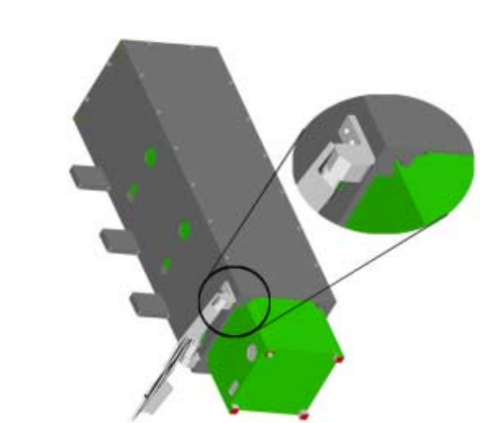
\includegraphics[width=0.7\textwidth]{figuras/ppod_explodido.png}
  \end{center}
  \fonte{Adaptado de Puig-Suari, Turner e Ahlgren (2002).}
\end{figure}

Do ponto de vista cinemático e tribológico, o confinamento no P-POD impõe que os quatro cantos longitudinais do CubeSat atuem como trilhos-guia deslizantes no interior das canaletas tubulares. Na montagem de voo e em ensaios de qualificação em mesas vibratórias acopladas a casulos de ensaio (\textit{Test POD}), os trilhos não são engastados, mas sim restringidos por contato mecânico unilateral sujeito a uma folga diametral nominal (\textit{clearance} de \SIrange{0.1}{0.3}{\milli\metre}), apoiando-se axialmente na interface inferior de sapatas e pinos de encosto da base ($Z = 0$). Durante os ensaios de vibração estocástica e transientes de lançamento, essa folga construtiva induz fenômenos de descolamento periódico, impacto intermitente e vibração com folga (\textit{chattering}), os quais alteram a resposta dinâmica linear do sistema e reduzem a primeira frequência natural aparente em relação a condições idealizadas de engastamento perfeito. Restrições estritas de tolerância dimensional e a necessidade de prevenir o travamento mecânico (\textit{jamming}) ou a microssoldagem a frio sob alto vácuo exigem que esses trilhos tenham seção sólida de \rail{}, cantos arredondados ($R \ge \SI{1.0}{\milli\metre}$) e acabamento superficial com anodização dura tipo III (PTFE impregnado) com rugosidade $Ra \le \SI{1.6}{\micro\metre}$ (PUIG-SUARI \textit{et al.}, 2002). Consequentemente, torna-se geometricamente mandatório que os trilhos do nanossatélite permaneçam maciços e contínuos, de modo que a otimização de alívio de massa e atenuação vibratória seja direcionada exclusivamente aos painéis internos do chassi.

O evento de ejeção é deflagrado pela liberação da porta frontal do dispensador, descarregando a energia potencial elástica acumulada na mola helicoidal principal sobre a placa empurradora (\textit{pusher plate}). A dinâmica translacional de ejeção do satélite ao longo do curso de ejeção é governada pela equação de movimento expressa na Equação~\eqref{eq:ejecao} (LIMA; MANEA; SANTOS, 2021):
\begin{equation}
  M\,\ddot{z} + \mu N \operatorname{sgn}(\dot{z}) = P_0 - c\,z
  \label{eq:ejecao}
\end{equation}
em que $M$ denota a massa combinada do CubeSat e da plataforma empurradora, $\ddot{z}$ representa a aceleração axial instantânea, $P_0$ é a pré-carga inicial da mola comprimida, $c$ é a constante de rigidez da mola, $\mu$ é o coeficiente de atrito cinemático contra as guias do tubo, $N$ é a força normal de contato induzida por desalinhamentos e $z$ corresponde ao deslocamento axial percorrido até o curso total ($z = z_{\text{curso}}$). 

Ao término do curso de impulsão, a placa empurradora desacelera bruscamente ao colidir contra o batente mecânico final do dispensador, transferindo um pulso transiente de choque impulsivo de curta duração ($\Delta t \sim \SIrange{1}{3}{\milli\second}$) que se propaga pelos trilhos do nanossatélite no instante de sua liberação em órbita livre (LIMA \textit{et al.}, 2021). A severidade desse evento dinâmico é quantificada pelo Espectro de Resposta ao Choque (\textit{Shock Response Spectrum} -- SRS, com fator de qualidade $\mathcal{Q} = 10$), impondo acelerações de pico que podem superar \SI{500}{\gacc} em frequências superiores a \SI{1000}{\hertz}.

Adicionalmente, esse impulso inicial excita a dinâmica de múltiplos corpos acoplados do satélite. Em plataformas providas de apêndices flexíveis articulados, como hastes de magnetômetros (\textit{booms}), antenas de comunicação e painéis solares dobráveis, o choque de ejeção pode excitar frequências modais ressonantes dos mecanismos periféricos (MANTOVANI; SANTOS; CARDOSO-RIBEIRO, 2020). Essa interação dinâmica reforça a exigência de que os painéis do chassi primário possuam capacidade passiva intrínseca de filtragem mecânica e atenuação de ondas elásticas, evitando a propagação de transientes de alta frequência que possam danificar as articulações dos apêndices ou descalibrar componentes ópticos.

\section{Metamateriais auxéticos e estruturas híbridas de alto desempenho}
\label{sec:auxeticos}

Para superar a baixa dissipação de energia dos materiais monolíticos contínuos, a engenharia de estruturas tem incorporado metamateriais celulares com coeficiente de Poisson negativo ($\nu < 0$), denominados auxéticos. A caracterização empírica de colmeias metálicas reentrantes bidimensionais manufaturadas por fusão seletiva a laser (SLM) em ligas de alumínio foi investigada por Alomarah \textit{et al.} (2017). Esses autores demonstraram que a resposta mecânica e a magnitude do coeficiente de Poisson negativo dessas matrizes exibem acentuada anisotropia direcional: espécimes solicitados na direção X apresentam rigidez e limites de escoamento consideravelmente inferiores aos observados na direção Y. Corroborando essa dependência direcional no contexto da manufatura aditiva metálica, Ermurat e Da\u{g} (2025) avaliaram a influência combinada da orientação de construção (\textit{build orientation}) e do sentido de aplicação de carga sobre o comportamento compressivo de estruturas auxéticas reentrantes manufaturadas aditivamente. As investigações evidenciaram que o arranjo das camadas depositadas afeta substancialmente os modos de deformação plástica, a capacidade de absorção energética e a suscetibilidade a concentrações locais de tensão nos vértices nodais.

Além da anisotropia elástica e da dependência em relação à orientação de fabricação, matrizes reentrantes convencionais fabricadas por manufatura aditiva sem pós-processamento térmico sofrem de limitações severas de ductilidade. Como verificado experimentalmente por Alomarah \textit{et al.} (2017), a concentração de deformações plásticas nas quinas internas das costelas oblíquas induz a formação prematura de trincas e fratura frágil sob carregamentos quase estáticos, inibindo o desenvolvimento de um platô plástico estendido de absorção energética. A Figura~\ref{fig:falha-reentrante} ilustra os modos típicos de colapso e a propagação de trincas nas junções de células reentrantes 2D sob tração uniaxial.

\begin{figure}[htb]
  \caption{Modos de falha e comportamento cinemático anisotrópico de célula reentrante 2D sob carregamento uniaxial}
  \label{fig:falha-reentrante}
  \begin{center}
    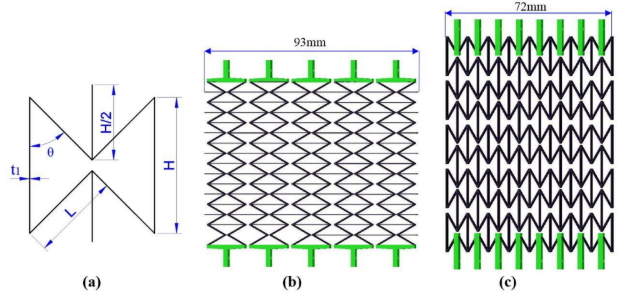
\includegraphics[width=0.85\textwidth]{figuras/modos_falha_reentrante.png}
  \end{center}
  \fonte{Adaptado de Alomarah \textit{et al.} (2017).}
\end{figure}

Para contornar o colapso localizado e estender a capacidade de absorção de choque, geometrias celulares avançadas combinam mecanismos reentrantes com elementos quirais ou bioinspirados. Cui, Zhang e Wang (2025) demonstraram que a incorporação de núcleos quirais rotacionais no interior de colmeias reentrantes, conforme ilustrado na Figura~\ref{fig:hibrida-quiral}, propicia um aumento de até \SI{95}{\percent} na Absorção Específica de Energia (\textit{Specific Energy Absorption} -- SEA) em comparação com topologias puramente reentrantes. 

\begin{figure}[htb]
  \caption{Topologia híbrida de célula celular com elementos quirais internos acoplados a paredes reentrantes}
  \label{fig:hibrida-quiral}
  \begin{center}
    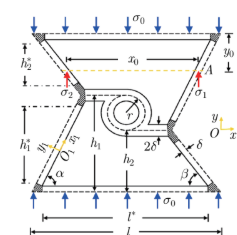
\includegraphics[width=0.55\textwidth]{figuras/celula_hibrida_quiral.png}
  \end{center}
  \fonte{Adaptado de Cui, Zhang e Wang (2025).}
\end{figure}

Apesar do incremento expressivo de absorção de energia propiciado pelas células híbridas quirais reportadas por Cui, Zhang e Wang (2025), tais geometrias impõem severos desafios de fabricabilidade no processo de fusão em leito de pó a laser (L-PBF). A geometria dos nós circulares e ligamentos curvos rotacionais resulta frequentemente em superfícies suspensas com ângulos de inclinação (\textit{overhang}) críticos inferiores a \SI{35}{\degree}, exigindo suportes sacrificiais internos que se tornam inacessíveis para remoção mecânica após a consolidação a laser. Em adição, a complexidade dos canais internos confinados dificulta a evacuação e a recuperação do pó metálico não fundido. Em contrapartida, a célula unitária tridimensional reentrante (3D \textit{re-entrant}) selecionada no presente estudo assegura plena conformidade com as diretrizes de \textit{Design for Additive Manufacturing} (DfAM): a parametrização das costelas garante ângulos de sobressalto $\theta_{\text{overhang}} \ge \SI{35}{\degree}$ ao longo da direção de construção vertical, dispensando integralmente suportes internos sacrificiais e mantendo canais desobstruídos e contínuos para drenagem e despoeiramento em L-PBF.

Sob o ponto de vista da elastodinâmica, tais arranjos arquitetados atuam de maneira análoga a cristais fonônicos, exibindo zonas de atenuação espectral (\textit{phononic bandgaps}) que impedem a transmissão de ondas elásticas em faixas específicas de frequência (LI \textit{et al.}, 2026; FARSHBAF \textit{et al.}, 2025). Essa propriedade física viabiliza o isolamento mecânico passivo de cargas úteis de alta sensibilidade, dispensando o uso de amortecedores elastoméricos adicionais que poderiam degradar por desgaseificação (\textit{outgassing}) no ambiente espacial.

\section{\textit{Design for Additive Manufacturing} (DfAM) e modelos de escala}
\label{sec:dfam}

A viabilização prática de componentes espaciais celulares é intrinsecamente governada pelo paradigma de \textit{Design for Additive Manufacturing} (DfAM). Conforme destacado na revisão de Khan e Riccio (2024), processos de Manufatura Aditiva por Fusão em Leito de Pó a Laser (\textit{Laser Powder Bed Fusion} -- L-PBF) proporcionam liberdade geométrica para a confecção de Estruturas de Densidade Graduada (\textit{Functionally Graded Lattices} -- FGL). A modulação espacial contínua da espessura das costelas e da porosidade celular viabiliza a concentração de rigidez onde os fluxos de tensão são mais intensos, aliviando massa em regiões subutilizadas.

Para estimar a rigidez macroscópica de meios celulares sem recorrer a simulações de malha contínua refinada em cada iteração de projeto, utilizam-se classicamente as leis fenomenológicas de escala propostas por Gibson e Ashby (1997). A relação analítica fundamental correlaciona o módulo de elasticidade efetivo homogeneizado ($E^{*}$) com a densidade relativa da estrutura ($\rho^{*}/\rho_s$) por uma lei de potência:
\begin{equation}
  \frac{E^{*}}{E_s} = C \left( \frac{\rho^{*}}{\rho_s} \right)^{n}
  \label{eq:gibson}
\end{equation}
na qual $E_s$ e $\rho_s$ representam o módulo de Young e a massa específica do material metálico sólido de base, e $C$ e $n$ são constantes empíricas dependentes da topologia celular. Para arquiteturas celulares cujo modo predominante de deformação sob carga elástica é a flexão das costelas oblíquas — caso das células reentrantes —, adota-se classicamente $n \approx 2$ (ZHONG \textit{et al.}, 2023).

Todavia, investigações recentes apontam desvios significativos do modelo clássico de Gibson-Ashby em componentes manufaturados por L-PBF. Zhong \textit{et al.} (2023) salientam que a Equação~\eqref{eq:gibson} assume a hipótese de vigas esbeltas de Euler-Bernoulli, válida apenas para baixas densidades relativas ($\rho^{*}/\rho_s < \num{0.3}$) e razões comprimento-diâmetro de haste $L/D > 5$. Em contrapartida, estruturas otimizadas para satélites operam frequentemente com densidades relativas moderadas e elevadas ($\rho^{*}/\rho_s \ge \num{0.35}$), regime no qual os esforços axiais e o cisalhamento transversal tornam-se preponderantes.

Conforme demonstrado por Zimmerman \textit{et al.} (2026), o modelo clássico de potência perde precisão analítica no limite do sólido maciço ($\rho^{*}/\rho_s \to 1$), uma vez que não prevê a transição assintótica da resposta governada pela cinemática celular para o comportamento constitutivo do material contínuo. Além disso, irregularidades geométricas microestruturais inerentes ao L-PBF — tais como rugosidade superficial em superfícies inclinadas, aderência de partículas de pó semidilatadas e variações locais no diâmetro do feixe de laser — degradam a rigidez efetiva em comparação com geometrias computacionais ideais (ZIMMERMAN \textit{et al.}, 2026).

Para incorporar esses efeitos e restabelecer a precisão analítica em meios celulares graduados, Beigrezaee, Jalali e Pugno (2026) desenvolveram uma formulação corrigida baseada na introdução de parâmetros modificadores:
\begin{equation}
  \frac{E^{*}}{E_s} = \alpha\,\beta\,C \left( \frac{\rho^{*}}{\rho_s} \right)^{n}
  \label{eq:refinado}
\end{equation}
em que $\alpha$ é o coeficiente de correção determinístico para o gradiente de espessura de parede ao longo do volume, e $\beta$ quantifica o fator de degradação elástica oriundo de imperfeições estocásticas e porosidades induzidas pelo processo de fusão aditiva (BEIGREZAEE \textit{et al.}, 2026). A calibração dos fatores $\alpha$ e $\beta$ permite ancorar as previsões do modelo substituto neural em bases fenomenológicas sólidas.

\section{Integridade estrutural e fadiga em estruturas celulares}
\label{sec:fadiga}

A qualificação aeroespacial de um chassi primário em liga de AlSi10Mg fabricado por L-PBF requer a garantia estrita de resistência mecânica contra a fadiga vibracional estocástica imposta pelo veículo lançador (SLEJKO \textit{et al.}, 2023). Em estruturas celulares metálicas, a presença de descontinuidades geométricas e microestruturais — tais como porosidade por aprisionamento de gás, falta de fusão interfacial e rugosidade superficial dispersa — impede o uso de abordagens clássicas baseadas em fatores teóricos de concentração de tensões elásticas ($K_t$) ou tensões nominais médias (COLLINI; MENEGHETTI, 2024).

Para superar essa limitação e estabelecer uma metodologia de dimensionamento tolerante a defeitos (\textit{defect-tolerant design}), adota-se a formulação da Mecânica da Fratura Linear Elástica (LEFM). Conforme demonstrado por Collini e Meneghetti (2024), as junções nodais e reentrâncias das células podem ser modeladas como entalhes geométricos agudos em V com raio de ponta pequeno, sendo o campo de tensões locais descrito pelo Fator de Intensidade de Tensão de Entalhe (\textit{Notch Stress Intensity Factor} -- NSIF) em Modo I:
\begin{equation}
  \Delta K_1^{V} = \sqrt{2\pi}\,\lim_{r \to 0} \left[ \Delta\sigma_{\theta\theta}(r)\; r^{\,1-\lambda_1} \right]
  \label{eq:nsif}
\end{equation}
em que $\Delta K_1^{V}$ representa a amplitude do NSIF em Modo I, $\Delta\sigma_{\theta\theta}$ é a componente de tensão normal circunferencial atuante a uma distância radial $r$ do vértice do entalhe, e $1-\lambda_1$ denota a ordem da singularidade elástica assintótica de Williams, dependente do ângulo de abertura do entalhe nodal.

A integração da abordagem LEFM acoplada ao Método da Tensão de Pico (\textit{Peak Stress Method} -- PSM) em modelos de elementos finitos permite correlacionar o estado de tensão nodal gerado pela vibração aleatória diretamente com o limiar de propagação de trincas por fadiga da liga AlSi10Mg ($\Delta K_{th} = \SI{2.5}{\mega\pascal\sqrt{\metre}}$) (COLLINI; MENEGHETTI, 2024). Assim, o processo de otimização topológica assegura que as tensões estocásticas de pico ($3\sigma$) nos nós da estrutura permaneçam estritamente abaixo do limiar de propagação, garantindo a integridade do componente durante a fase de qualificação de voo.

\section{Modelos substitutos neurais guiados por física e sistemas multiagente na engenharia aeroespacial}
\label{sec:pgnn-agentes}

A determinação das geometrias celulares ótimas por meio de algoritmos evolutivos multiobjetivo, como o NSGA-II (DEB \textit{et al.}, 2002), impõe a execução de dezenas de milhares de avaliações de candidatas. A realização direta desse volume de simulações por Elementos Finitos (FEA) tridimensionais em malhas refinadas de paredes celulares delgadas é computacionalmente impraticável, exigindo horas de processamento para cada solução (ZHENG \textit{et al.}, 2024).

Para contornar esse gargalo, empregam-se Modelos Substitutos (\textit{surrogates}) treinados com aprendizado profundo. Para mitigar o risco de predições fisicamente espúrias ou de extrapolações não monotônicas intrínsecas a modelos empíricos de caixa preta, a metodologia deste trabalho estrutura uma Rede Neural Guiada por Física (\textit{Physics-Guided ResNet}). A função de perda supervisionada composta incorpora penalidades fenomenológicas diretamente durante o treinamento:
\begin{equation}
  \mathcal{L}_{\text{total}} = \mathcal{L}_{\text{MSE}} + \lambda_{\text{phys}}\,\mathcal{L}_{\text{Gibson-Ashby}} + \lambda_{\text{mono}}\,\mathcal{L}_{\text{monotonicidade}}
  \label{eq:perda-conceito}
\end{equation}
em que $\mathcal{L}_{\text{MSE}}$ quantifica o erro quadrático médio em relação ao conjunto de simulações numéricas de alta ordem (Ansys MAPDL), $\mathcal{L}_{\text{Gibson-Ashby}}$ penaliza desvios assintóticos das leis de escala celulares para regimes de baixa densidade, e $\mathcal{L}_{\text{monotonicidade}}$ impõe que acréscimos na espessura de parede das células promovam elevações estritamente monótonas na rigidez efetiva e na primeira frequência própria fundamental ($f_1$).

Para governar a interação entre triagem geométrica, inferência neural e checagem de conformidade normativa, adota-se o paradigma de Grafos de Estados Finitos Determinísticos (\textit{Deterministic StateGraph Workflow}) implementado por meio da biblioteca LangGraph. Ao contrário de arquiteturas de agentes reativos baseados em modelos de linguagem com tomadas de decisão probabilísticas, o pipeline aqui desenvolvido opera como um Grafo Acíclico Dirigido (DAG) estritamente determinístico, fundado sobre contratos de dados imutáveis e fortemente tipados (\code{CubeSatState}). Esse arranjo desacopla o fluxo em nós especialistas com responsabilidade única: o portão de manufaturabilidade aditiva (\code{CadDfamAgent}), o estimador dinâmico neural de submilissegundos (\code{NeuralSurrogateAgent}) e o módulo de qualificação ambiental espacial (\code{GevsQualifierAgent}), coordenados pelo controlador supervisor (\code{OrchestratorAgent}). 

Na engenharia de sistemas espaciais e computação científica de alto desempenho, fluxos determinísticos dessa natureza são tradicionalmente geridos por orquestradores de tarefas como Prefect, Snakemake ou Apache Airflow, os quais se destacam na execução distribuída em clusters HPC e gerenciamento de cache. No presente arcabouço, a seleção do LangGraph fundamenta-se na facilidade de instanciação de máquinas de estados tipadas em Python puro, com suporte nativo a bifurcações condicionais (\textit{fail-fast routing}), pontos de controle de persistência de estado (\textit{checkpoints}) e manutenção de uma trilha de auditoria contínua (\textit{execution audit trail}) com carimbos UTC e justificativas técnicas de descarte. Esse arranjo computacional assegura rastreabilidade irrestrita, elimina precocemente candidatos inviáveis antes de processamentos numéricos custosos e garante que apenas geometrias física e normativamente homologadas componham a fronteira de Pareto.

\section{Síntese da revisão e definição de requisitos}
\label{sec:requisitos}

A consolidação da fundamentação teórica orienta a formulação da Matriz de Requisitos de Engenharia de Sistemas para o chassi primário do nanossatélite CubeSat 1U, sintetizada na Tabela~\ref{tab:requisitos}. A conversão das normas ambientais (NASA GEVS) e das interfaces cinemáticas operacionais (P-POD) em restrições quantitativas delimita o espaço de busca e estabelece os critérios objetivos de sucesso para as fases metodológicas subsequentes.

\begin{table}[htb]
  \caption{Matriz de requisitos de engenharia de sistemas para o chassi do CubeSat 1U}
  \label{tab:requisitos}
  \footnotesize
  \SingleSpacing
  \begin{tabularx}{\textwidth}{@{}>{\raggedright\arraybackslash}p{1.6cm} >{\raggedright\arraybackslash}p{2.2cm} >{\raggedright\arraybackslash}p{2.4cm} >{\raggedright\arraybackslash}p{3.0cm} >{\raggedright\arraybackslash}X@{}}
    \toprule
    \textbf{ID} & \textbf{Requisito} & \textbf{Origem normativa} & \textbf{Métrica de projeto} & \textbf{Impacto no dimensionamento mecânico} \\
    \midrule
    REQ-EST-01 & Rigidez estrutural mínima & NASA GEVS (GSFC-STD-7000A) & Primeira frequência fundamental $f_1 \ge \SI{100.0}{\hertz}$ & Desacopla dinamicamente o satélite dos modos de empuxo do foguete; atua como restrição inferior ativa na otimização. \\[4pt]
    REQ-EST-02 & Resistência à vibração estocástica & NASA GEVS (GSFC-STD-7000A) & Qualificação sob excitação PSD de \SI{14.1}{\Grms} (\SIrange{20}{2000}{\hertz}) & Define o espectro de entrada na base; estabelece o critério para a verificação de fadiga estocástica de Steinberg e NSIF nos nós. \\[4pt]
    REQ-INT-01 & Envelopamento geométrico & CDS CalPoly (Rev. 14) & Dimensões nominais: \SI{100.0}{\milli\metre} $\times$ \SI{100.0}{\milli\metre} $\times$ \SI{113.5}{\milli\metre} ($\pm\,\SI{0.1}{\milli\metre}$) & Delimita o envelope volumétrico externo do chassi 1U; restringe a expansão dimensional das células auxéticas. \\[4pt]
    REQ-INT-02 & Continuidade cinemática nos trilhos & Dispensador P-POD (PUIG-SUARI \textit{et al.}, 2002) & Quatro trilhos contínuos de \rail{} com cantos $R \ge \SI{1.0}{\milli\metre}$ & Impõe arquitetura híbrida: arestas monolíticas maciças para deslizamento cinemático e painéis internos celulares. \\[4pt]
    REQ-INT-03 & Acabamento tribológico & Dispensador P-POD (PUIG-SUARI \textit{et al.}, 2002) & Rugosidade $Ra \le \SI{1.6}{\micro\metre}$ e anodização dura Tipo III & Mitiga atrito seco e previne microssoldagem a frio sob alto vácuo durante a ejeção orbital. \\[4pt]
    REQ-MNC-01 & Alocação de massa estrutural & CDS CalPoly (Rev. 14) & Massa total do satélite $\le \SI{1.33}{\kilo\gram}$ (chassi primário $\le \SI{0.350}{\kilo\gram}$) & Exige núcleos celulares auxéticos de densidade graduada para atingir massa estrutural inferior a \SI{0.150}{\kilo\gram}. \\[4pt]
    REQ-DIF-01 & Suporte a choque de ejeção & Dinâmica transiente P-POD (LIMA \textit{et al.}, 2021) & Suportar força de pré-carga impulsiva da mola ($P_0$) com atrito dinâmico & Define as condições de contorno de lançamento e aceleração máxima de liberação translacional. \\
    \bottomrule
  \end{tabularx}
  \fonte{Elaborada pelo autor (2026), adaptada de NASA (2013), California Polytechnic State University (2022), Puig-Suari \textit{et al.} (2002) e Lima \textit{et al.} (2021).}
\end{table}

A satisfação estrita desses requisitos governa a formulação multiobjetivo executada nas etapas seguintes da pesquisa, tendo como meta precípua maximizar a atenuação dinâmica de aceleração RMS nas interfaces da carga útil e minimizar a massa estrutural, com garantia de Margem de Segurança estática positiva ($MS_{\text{yield}} > 0$) e índice de dano cumulativo de Steinberg estritamente inferior ao teto de qualificação espacial ($D \le \num{0.25}$).

\chapter{Metodologia}
\label{cap:metodologia}
% --------------------------------------------------------------------------

Este capítulo detalha o rigor metodológico aplicado ao desenvolvimento, à aceleração neural e à validação do chassi primário auxético para nanossatélites CubeSat 1U. A pesquisa estrutura-se sobre uma abordagem computacional integrada que combina a análise dimensional celular, a modelagem multiescala por elementos de volume representativo (RVE), a síntese paramétrica B-Rep com restrições de Manufatura Aditiva (DfAM) e simulações elastodinâmicas de alta fidelidade em elementos finitos no ecossistema aberto (Code\_Aster e Gmsh Tet10 em ambiente Linux/WSL). O fluxo operacional está dividido em quatro fases sequenciais: (i) ancoragem constitutiva direta na liga aeroespacial AlSi10Mg e parametrização geométrica; (ii) modelagem de contorno e homogeneização assintótica; (iii) simulação dinâmica normatizada em código aberto e síntese do modelo substituto neural guiado por física (\textit{Physics-Guided ResNet}); e (iv) validação de alta ordem (\textit{Code\_Aster Ground Truth}) e integridade à fadiga estocástica.

\section{Princípio de similaridade mecânica, análise dimensional e limites de transferibilidade}
\label{sec:similaridade}

A formulação teórica de escala para metamateriais celulares fundamenta-se na Teoria da Similaridade Mecânica e na análise dimensional governada pelo Teorema Pi de Buckingham (NASA, 2016). Esse princípio estabelece que sistemas físicos governados pelos mesmos fenômenos constitutivos preservam relações dinâmicas invariantes quando os grupos adimensionais característicos são estritamente conservados.

No domínio dos metamateriais celulares e estruturas treliçadas, a variável adimensional governante primária é a densidade relativa ($\rho^{*}/\rho_s$), que define a fração de volume ocupada pelo material sólido e dita a rigidez elástica equivalente ($E^{*}/E_s$). De acordo com as leis fundamentais de Gibson e Ashby (1997), a relação constitutiva macroscópica para matrizes celulares dominadas por flexão é regida pela lei de potência formulada na Equação~\eqref{eq:pi1}:
\begin{equation}
  \Pi_1 = \frac{E^{*}}{E_s} = C \left( \frac{\rho^{*}}{\rho_s} \right)^{n}
  \label{eq:pi1}
\end{equation}
na qual $C$ e $n$ são constantes topológicas puras associadas à cinemática de deformação da célula unitária reentrante.

Para o comportamento elastodinâmico e o desacoplamento ressonante no veículo lançador, a formulação dimensional define o segundo grupo adimensional ($\Pi_2$), correlacionando a frequência natural fundamental ($f_n$), a dimensão característica macroscópica ($L$) e as propriedades mecânicas eficazes:
\begin{equation}
  \Pi_2 = f_n \cdot L \sqrt{\frac{\rho^{*}}{E^{*}}} = \text{constante} \quad \implies \quad f_n \propto \frac{1}{L} \sqrt{\frac{E^{*}}{\rho^{*}}}
  \label{eq:fn}
\end{equation}

Contudo, sob o rigor estrito da qualificação estrutural aeroespacial, é imperativo explicitar os limites físicos de validade dessa abordagem dimensional. Embora a similaridade elástica linear clássica governada por $\Pi_1$ e $\Pi_2$ forneça correlações consistentes para deformações estáticas e autovalores modais teóricos não amortecidos em meios homotéticos, ela configura uma \textbf{similaridade incompleta (\textit{incomplete similarity})} quando estendida à dinâmica estocástica de vibração aleatória e à integridade em fadiga. Existem divergências constitutivas intransponíveis entre domínios poliméricos (como termoplásticos impressos por FDM) e ligas metálicas aeroespaciais:
\begin{alineas}
  \item \textbf{amortecimento e dissipação interna de energia:} termoplásticos exibem comportamento viscoelástico pronunciado, com amortecimento interno fortemente dependente da taxa de deformação e temperatura ($\zeta_{\text{polímero}} \approx \num{0.03}$ a $\num{0.06}$, ou seja, $3\text{ a }6\%$), enquanto ligas metálicas aeroespaciais consolidadas por fusão a laser apresentam dissipação histerética muito inferior ($\zeta_{\text{AlSi10Mg}} \approx \num{0.005}$ a $\num{0.02}$, $0{,}5\text{ a }2\%$). Essa discrepância altera de forma radical o fator de amplificação dinâmica na ressonância ($Q = 1 / [2\zeta]$);
  \item \textbf{razão de rigidez e microestrutura celular:} a liga AlSi10Mg produzida por L-PBF exibe módulo de elasticidade cerca de 25 vezes superior ao de termoplásticos comerciais ($E_{\text{metal}} = \SI{68.0}{\giga\pascal}$ contra $E_{\text{polímero}} \approx \SI{2.5}{\giga\pascal}$ a $\SI{3.5}{\giga\pascal}$). Além disso, a microestrutura do metal solidificado por laser é formada por redes celulares eutéticas de silício finamente dispersas em matriz de alumínio, diferindo substancialmente da adesão térmica entre filamentos poliméricos;
  \item \textbf{sensibilidade a entalhes, porosidades térmicas e mecânica da fratura:} o processo L-PBF induz tensões residuais térmicas de tração decorrentes do ciclo térmico ultrarrápido de fusão/solidificação, além de microporosidades intrínsecas (defeitos de falta de fusão e poros de aprisionamento gasoso). Sob vibração aleatória estocástica, tais descontinuidades atuam como concentradores de tensão severos com mecanismo de propagação de trincas por fadiga de alto ciclo e fratura linear elástica frágil, ausentes na viscoelasticidade dúctil de polímeros.
\end{alineas}

Em face dessas distinções fenomenológicas, este trabalho descarta categoricamente qualquer tentativa de extrapolação empírica de respostas dinâmicas ou calibração de malha a partir de materiais plásticos. O emprego de modelos conceituais tridimensionais preliminares em filamento termoplástico (PLA) circunscreve-se estritamente à verificação física de empacotamento volumétrico e checagem dimensional de montagem (\textit{fit-check} virtual) nas interfaces dos trilhos do casulo lançador P-POD e placas de aviônica PC/104. Toda a modelagem constitutiva, o banco de dados de simulações elastodinâmicas e a qualificação espacial são ancorados de forma direta, unívoca e rigorosa nas propriedades da liga metálica de voo AlSi10Mg processada por L-PBF.

\section{Fases da metodologia}
\label{sec:fases}

\subsection{Ancoragem constitutiva na liga aeroespacial AlSi10Mg (L-PBF)}
\label{subsec:caracterizacao}

A primeira fase metodológica compreende a ancoragem constitutiva unívoca na liga aeroespacial AlSi10Mg aliviada termicamente ($300^\circ\text{C} / 2\text{ h}$), amplamente consolidada na indústria espacial para componentes estruturais fabricados por Fusão em Leito de Pó a Laser (L-PBF). Em conformidade com as normas internacionais de qualificação de materiais aeroespaciais e relatórios técnicos de caracterização aditiva (SLEJKO \textit{et al.}, 2023; KHAN; RICCIO, 2024), adotam-se as propriedades mecânicas canônicas listadas na Tabela~\ref{tab:propriedades-alsi10mg}.

\begin{table}[htb]
  \caption{Propriedades mecânicas e critérios de projeto da liga aeroespacial AlSi10Mg (L-PBF) com alívio térmico}
  \label{tab:propriedades-alsi10mg}
  \small
  \SingleSpacing
  \begin{tabularx}{\textwidth}{@{}>{\raggedright\arraybackslash}X >{\centering\arraybackslash}p{3.5cm} >{\centering\arraybackslash}p{4.0cm}@{}}
    \toprule
    \textbf{Propriedade termomecânica} & \textbf{Símbolo / Parâmetro} & \textbf{Valor adotado} \\
    \midrule
    Módulo de elasticidade longitudinal (Young) & $E$ & \SI{68.0}{\giga\pascal} \\
    Coeficiente de Poisson & $\nu$ & \num{0.33} \\
    Massa específica & $\rho$ & \SI{2670.0}{\kilo\gram\per\cubic\metre} \\
    Limite de escoamento convencional ($0{,}2\%$) & $\sigma_{\text{yield}}$ & \SI{230.0}{\mega\pascal} \\
    Limite de resistência à tração & $\sigma_{\text{ult}}$ & \SI{340.0}{\mega\pascal} \\
    Fator de segurança de qualificação (NASA GEVS) & $FS_{\text{yield}}$ & \num{1.25} \\
    Tensão admissível de projeto estocástico & $\sigma_{\text{adm}} = \sigma_{\text{yield}} / FS_{\text{yield}}$ & \SI{184.0}{\mega\pascal} \\
    Limiar de propagação de trincas por fadiga & $\Delta K_{th}$ & \SI{2.50}{\mega\pascal\sqrt{\metre}} \\
    \bottomrule
  \end{tabularx}
  \fonte{Elaborada pelo autor com base em Slejko \textit{et al.} (2023) e NASA (2013).}
\end{table}

No regime de pequenas deformações elásticas e vibração linear, o comportamento tridimensional do metal isotrópico contínuo é governado pela lei constitutiva generalizada de Hooke, expressa na Equação~\eqref{eq:hooke-3d}:
\begin{equation}
  \boldsymbol{\sigma} = \mathbf{C} : \boldsymbol{\varepsilon} = \lambda \operatorname{tr}(\boldsymbol{\varepsilon})\mathbf{I} + 2\mu\boldsymbol{\varepsilon}
  \label{eq:hooke-3d}
\end{equation}
na qual $\lambda$ e $\mu$ denotam os parâmetros elásticos de Lamé calculados a partir de $E$ e $\nu$:
\begin{equation}
  \lambda = \frac{E\,\nu}{(1+\nu)(1-2\nu)} = \SI{44.20}{\giga\pascal}, \qquad \mu = \frac{E}{2(1+\nu)} = G = \SI{25.56}{\giga\pascal}
  \label{eq:lame}
\end{equation}

Essa ancoragem direta nas constantes termomecânicas da liga metálica de voo elimina as incertezas e distorções constitutivas inerentes a extrapolações polímero-metal, assegurando que o espaço amostral do DoE, a inferência neural da ResNet e as margens de qualificação espacial da NASA GEVS reproduzam com alta fidelidade a física real do chassi primário de voo.

\subsection{Modelagem implícita e homogeneização assintótica}
\label{subsec:implicita}

A segunda fase da metodologia aborda a parametrização matemática e a redução computacional da estrutura celular. Cumpre explicitar a coexistência e os papéis complementares de duas representações geométricas no pipeline de desenvolvimento: a formulação implícita por superfícies de nível com base de Fourier (\textit{Fourier Level-Set}) representa o arcabouço teórico para a homogeneização analítica e o projeto de estruturas celulares com gradação funcional de densidade (\textit{Functionally Graded Lattices} -- FGL), viabilizando transições contínuas de densidade relativa; por sua vez, a síntese computacional em ambiente CAD via CadQuery/OpenCASCADE e a discretização por elementos finitos no Gmsh e Code\_Aster utilizam representação por contorno (\textit{Boundary Representation} -- B-Rep) governada pelo vetor explícito de parâmetros geométricos $\mathbf{x} = [\theta, t, l, h]^\top$.

No domínio analítico do \textit{Level-Set}, o domínio sólido $\Omega$ do metamaterial é definido pelo conjunto de pontos no espaço tridimensional delimitados pelo campo escalar contínuo $V(x,y,z)$, sujeito ao limiar de corte $t$:
\begin{equation}
  \Omega = \left\{ (x,y,z) \in \mathbb{R}^3 \;\middle|\; V(x,y,z) \le t \right\}, \qquad \partial\Omega = \left\{ (x,y,z) \in \mathbb{R}^3 \;\middle|\; V(x,y,z) = t \right\}
  \label{eq:iso}
\end{equation}
onde $\partial\Omega$ demarca a fronteira sólida externa da estrutura celular e o limiar $t$ modula diretamente a espessura média de parede e a densidade relativa local ($\rho^{*}/\rho_s$).

Para a célula unitária auxética reentrante tridimensional, cuja geometria paramétrica está apresentada na Figura~\ref{fig:celula-auxetica}, o campo de nível $V(x,y,z)$ é construído sobre uma base periódica de Fourier truncada de período cúbico $L$:
\begin{equation}
  \begin{aligned}
    V(x,y,z) ={}& \cos\!\left(\tfrac{2\pi x}{L}\right)\cos\!\left(\tfrac{2\pi y}{L}\right)
      + \cos\!\left(\tfrac{2\pi y}{L}\right)\cos\!\left(\tfrac{2\pi z}{L}\right)
      + \cos\!\left(\tfrac{2\pi z}{L}\right)\cos\!\left(\tfrac{2\pi x}{L}\right) \\
    & - \gamma \left[ \cos\!\left(\tfrac{2\pi x}{L}\right) + \cos\!\left(\tfrac{2\pi y}{L}\right) + \cos\!\left(\tfrac{2\pi z}{L}\right) \right]
  \end{aligned}
  \label{eq:fourier}
\end{equation}
onde o parâmetro $\gamma$ controla o grau de reentrância angular das paredes oblíquas, ditando a magnitude do coeficiente de Poisson negativo sob carregamento axial. A variação contínua da função de limiarização $t(x,y,z)$ possibilita a transição geométrica suave para uma Estrutura de Densidade Graduada (\textit{Functionally Graded Lattice} -- FGL), em estrita conformidade com as diretrizes de DfAM (KHAN; RICCIO, 2024).

Cumpre registrar com rigor conceitual que essa formulação analítica implícita baseada em superfícies de nível de Fourier atua nesta pesquisa estritamente como fundamentação teórica de referência contínua para o estado da arte em metamateriais e futuras expansões de otimização topológica inversa. Em contrapartida, toda a esteira computacional de síntese geométrica, checagens diagnósticas de fabricabilidade aditiva (DfAM), exportação no padrão industrial neutro STEP AP214 (ISO 10303-21) e discretização volumétrica de alta ordem no Gmsh adota deliberadamente a modelagem geométrica por contorno (\textit{Boundary Representation} -- B-Rep) governada pelo vetor paramétrico dimensional explícito $\mathbf{x} = [\theta, t, l, h]^\top$, detalhada na Seção~\ref{subsec:opencad-dfam}. Essa escolha de engenharia garante geometria analítica exata, previne artefatos espúrios de discretização de malha superficial e viabiliza a integração paramétrica monolítica entre as quatro faces celulares auxéticas e os quatro trilhos maciços do chassi CubeSat 1U (Figura~\ref{fig:cubesat-isometria}).

\begin{figure}[htb]
  \caption{Geometria e parametrização tridimensional da célula unitária auxética reentrante ($\theta, t, l, h$)}
  \label{fig:celula-auxetica}
  \begin{center}
    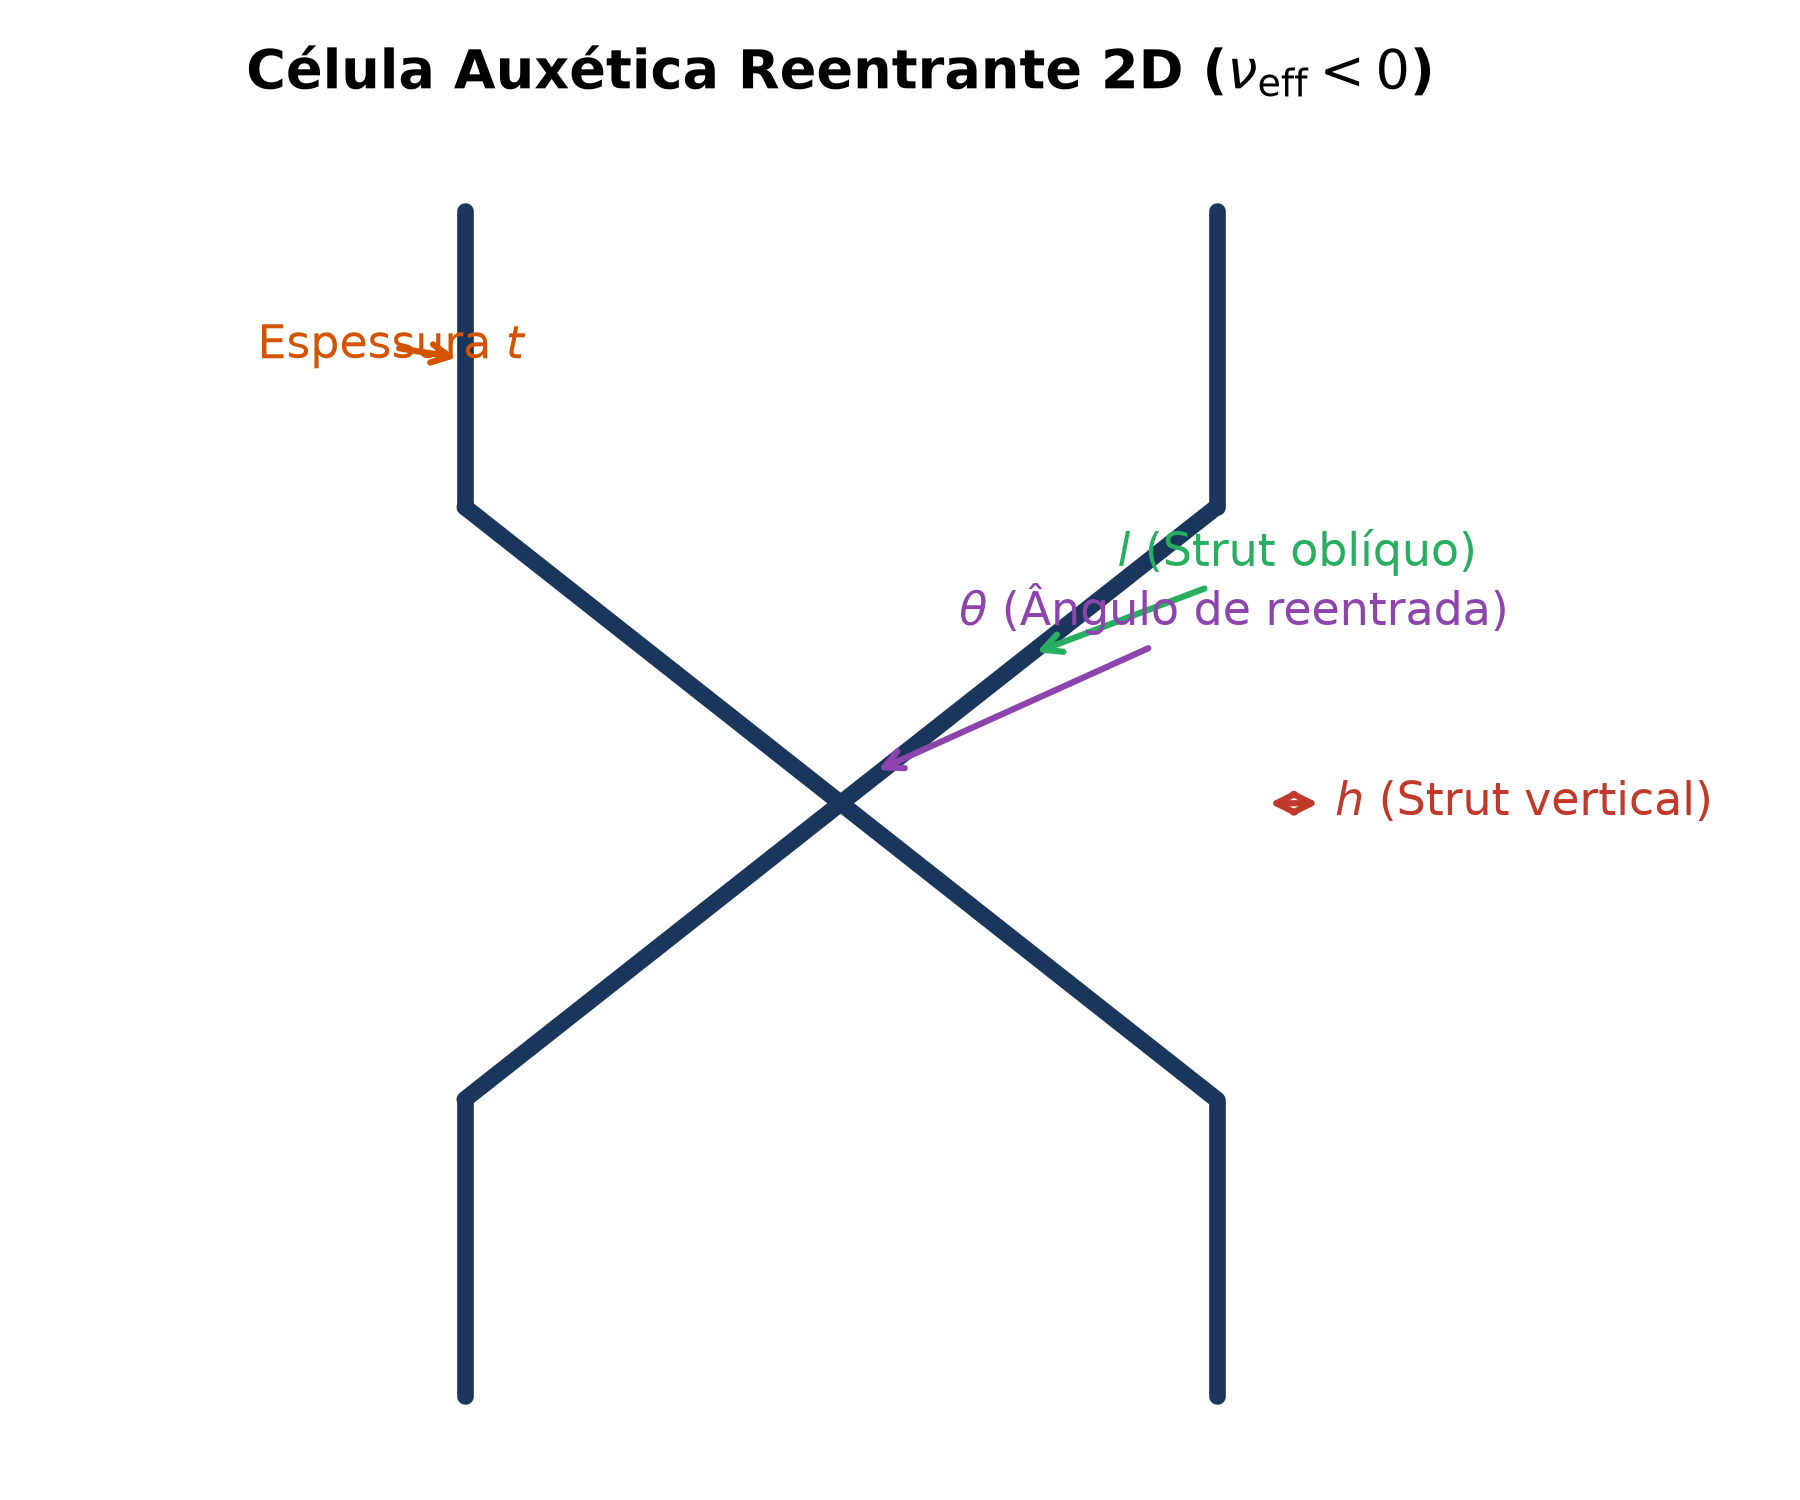
\includegraphics[width=0.7\textwidth]{figuras/auxetic_cell_geometry.png}
  \end{center}
  \fonte{Elaborada pelo autor (2026).}
\end{figure}

\begin{figure}[htb]
  \caption{Arquitetura estrutural híbrida do chassi CubeSat 1U: integração dos quatro trilhos maciços de contato P-POD (\SI{8.5}{\milli\metre}), painéis celulares auxéticos e envelope para barramento PC/104}
  \label{fig:cubesat-isometria}
  \begin{center}
    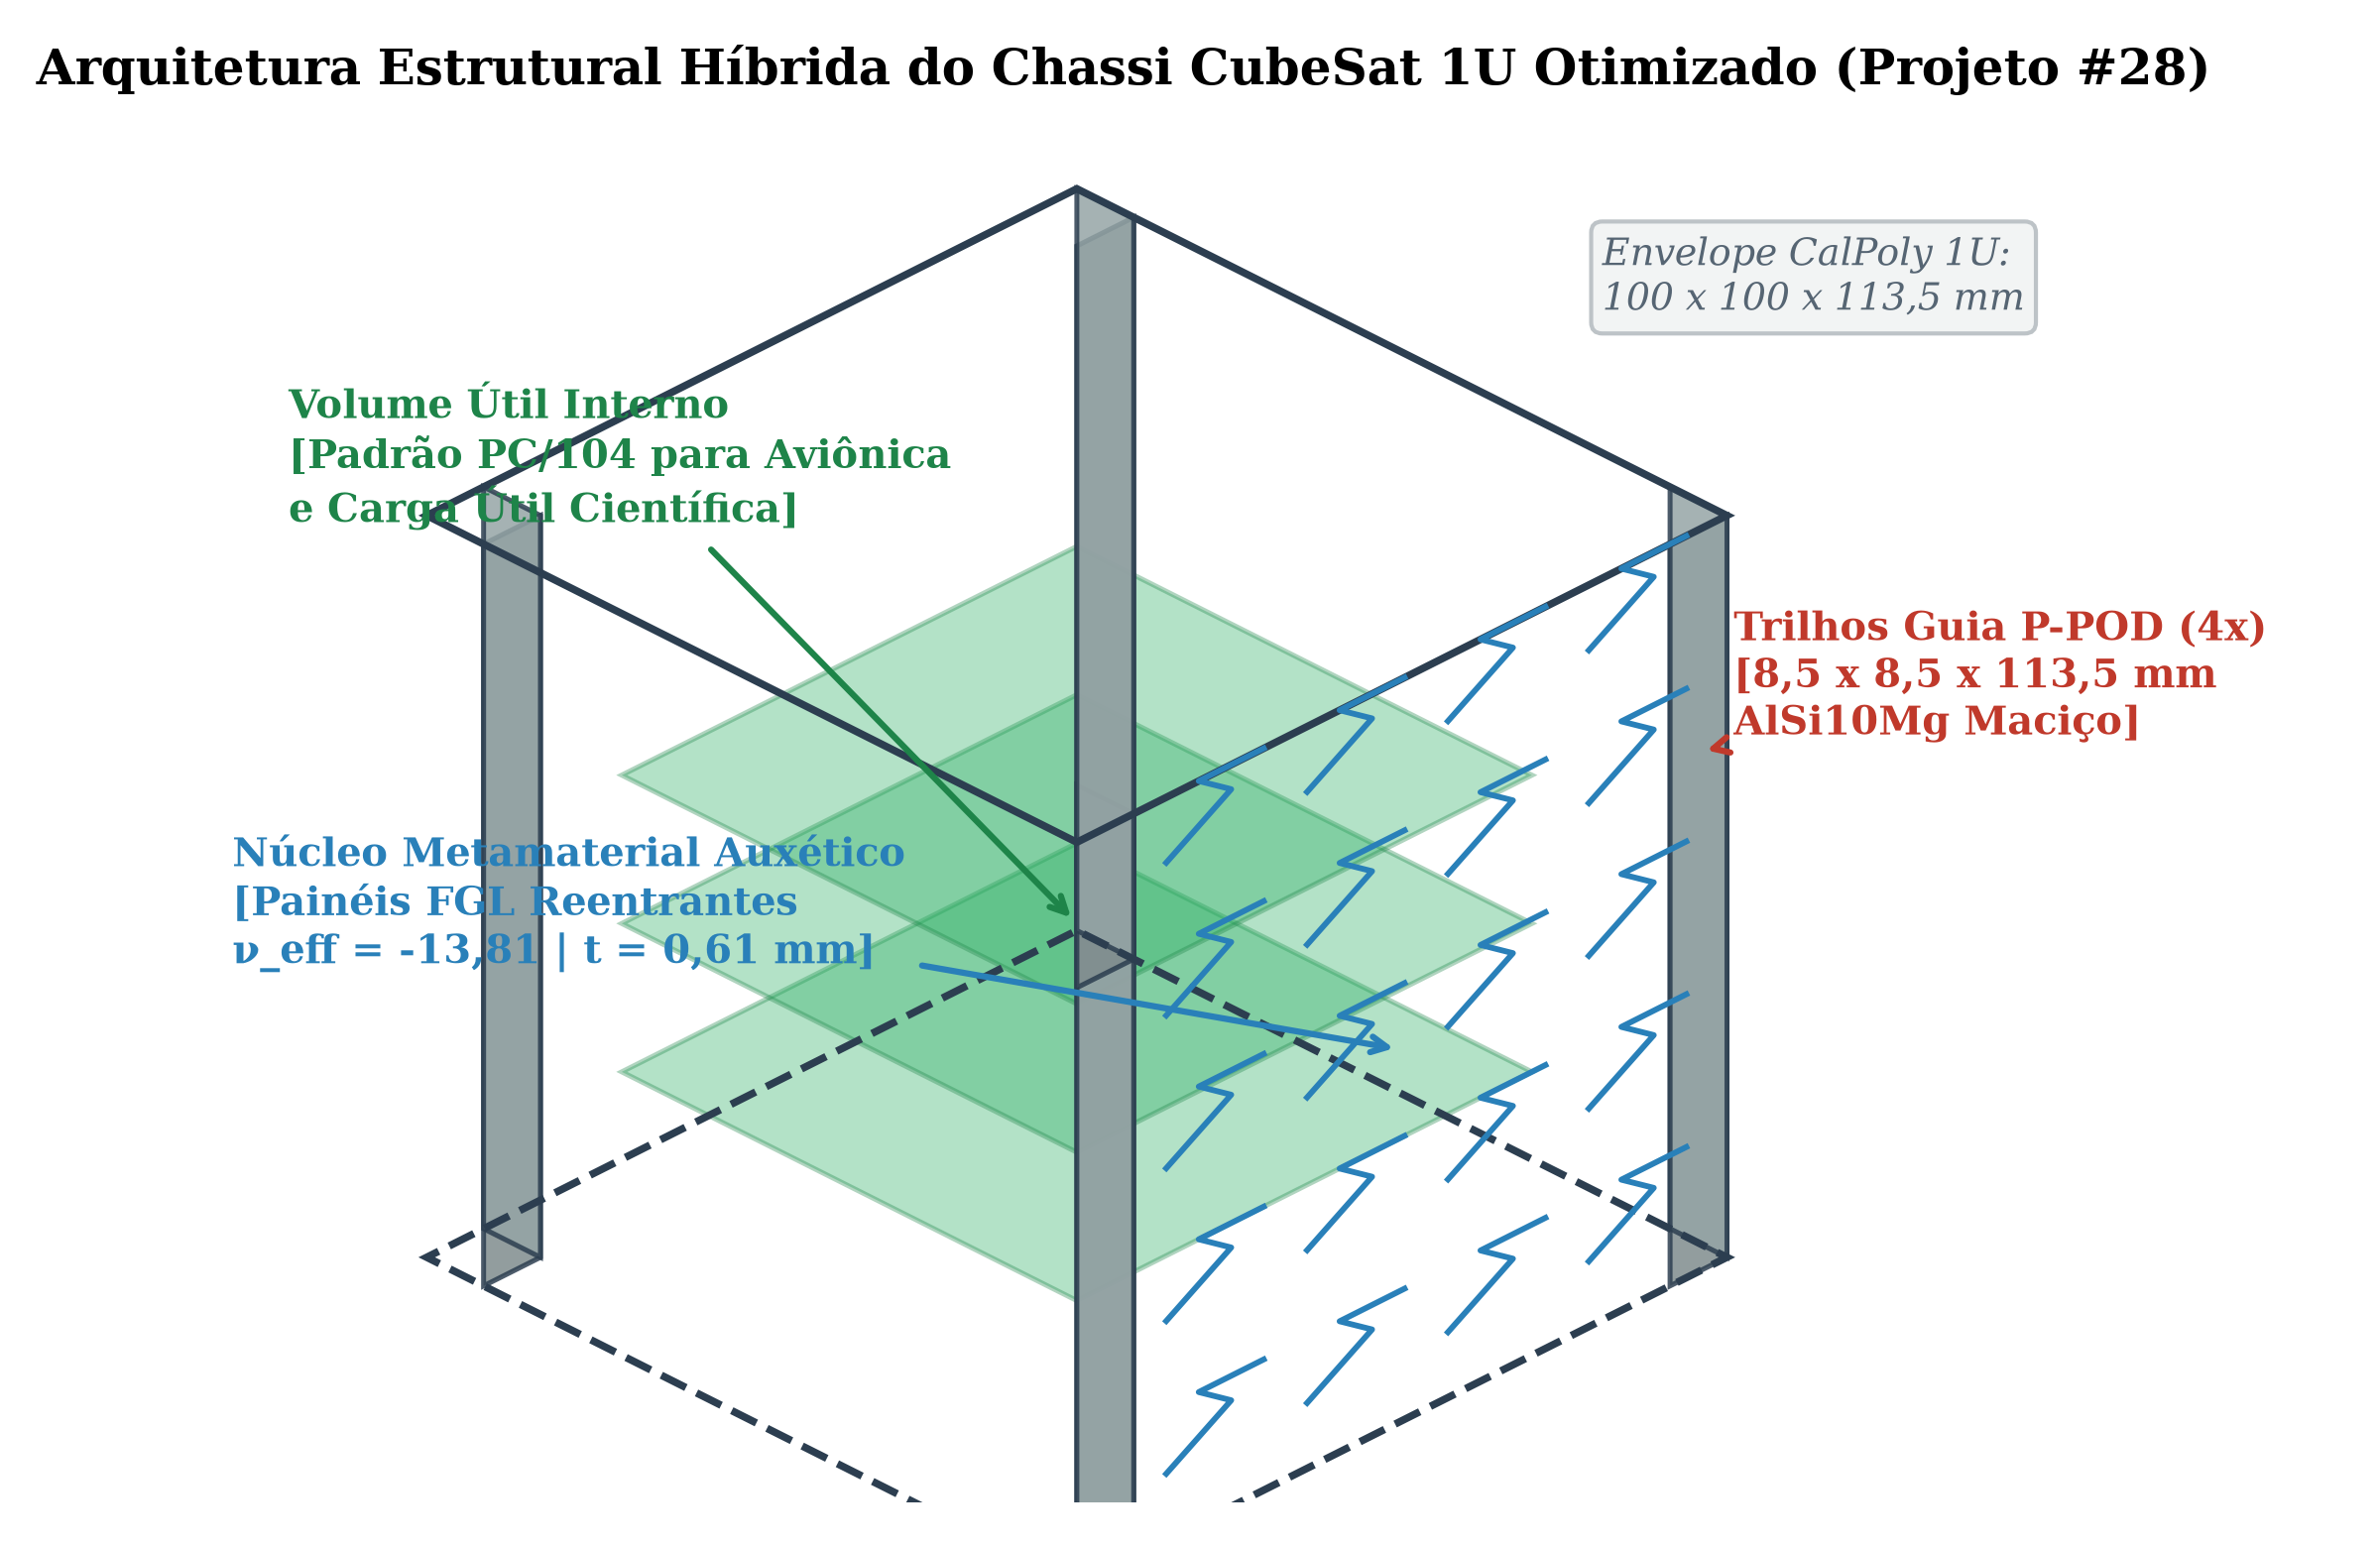
\includegraphics[width=0.85\textwidth]{figuras/cubesat_1u_isometric_assembly.png}
  \end{center}
  \fonte{Elaborada pelo autor (2026).}
\end{figure}

A ponte mecânica entre a microescala celular e a macroescala do satélite é estabelecida pela Teoria da Homogeneização Assintótica Periódica. A célula unitária é tratada como um Elemento de Volume Representativo (RVE) cúbico submetido a Condições de Contorno Periódicas (PBC) em pares de faces opostas:
\begin{equation}
  u_i^{+} - u_i^{-} = \bar{\varepsilon}_{ij} \left( x_j^{+} - x_j^{-} \right)
  \label{eq:pbc}
\end{equation}
onde $u_i^{+}$ e $u_i^{-}$ são os campos de deslocamento em nós conjugados das faces positiva e negativa do RVE, $\bar{\varepsilon}_{ij}$ é o tensor de deformações macroscópicas médias e $(x_j^{+} - x_j^{-})$ representa a distância vetorial entre as faces de contorno.

A extração do tensor de rigidez homogeneizado eficaz ($C_{ijkl}^{*}$) é realizada pelo cálculo da densidade média de energia de deformação elástica sobre o volume celular $|Y|$, submetendo o RVE a seis estados elementares de deformação unitária pura (três trações axiais e três cisalhamentos puros):
\begin{equation}
  C_{ijkl}^{*} = \frac{1}{|Y|} \int_{Y} C_{ijpq} \left( \varepsilon_{pq}^{0(kl)} - \varepsilon_{pq}\!\left(\chi^{(kl)}\right) \right) \mathrm{d}Y
  \label{eq:homog}
\end{equation}
em que $C_{ijpq}$ é o tensor constitutivo local do material de base, $\varepsilon_{pq}^{0(kl)}$ representa a deformação macroscópica unitária imposta e $\varepsilon_{pq}(\chi^{(kl)})$ corresponde ao campo de deformação flutuante periódico gerado pela presença dos vazios celulares. Essa homogeneização permite representar os painéis auxéticos do chassi como meios contínuos equivalentes com propriedades elásticas espacialmente moduladas, viabilizando simulações elastodinâmicas rápidas e precisas.

\subsubsection{Análise de dispersão fonônica e propagação de ondas via teorema de Bloch-Floquet}
\label{subsubsec:bloch}

Para comprovar matematicamente que a expressiva atenuação dinâmica da carga útil deriva de mecanismos elásticos de filtragem de ondas e incompatibilidade de impedância acústica (e não de uma taxa de amortecimento viscoso arbitrariamente inflada), formula-se a análise de propagação de ondas em meios periódicos infinitos tridimensionais com base no Teorema de Bloch-Floquet (BRILLOUIN, 1953; HUSSEIN; LEAMY; RUZZENE, 2014).

Considerando a célula unitária auxética reentrante de vetor de rede $\mathbf{R} = n_1 \mathbf{a}_1 + n_2 \mathbf{a}_2 + n_3 \mathbf{a}_3$ (com $n_i \in \mathbb{Z}$ e vetores de base ortogonais $\mathbf{a}_i$), a periodicidade espacial impõe que o campo de deslocamentos elásticos $\mathbf{u}(\mathbf{r}, t)$ sob propagação harmônica de frequência angular $\omega$ obedeça à condição de contorno periódica modulada em fase:
\begin{equation}
  \mathbf{u}(\mathbf{r} + \mathbf{R}) = \mathbf{u}(\mathbf{r}) e^{\mathrm{i} \mathbf{k} \cdot \mathbf{R}}
  \label{eq:bloch}
\end{equation}
em que $\mathbf{r} = (x, y, z)^\top$ é o vetor de posição contínuo, $\mathbf{k} = (k_x, k_y, k_z)^\top$ representa o vetor de onda de Bloch pertencente ao espaço recíproco e $\mathrm{i} = \sqrt{-1}$.

A discretização variacional da célula unitária pelo Método dos Elementos Finitos converte a equação de onda elástica elastodinâmica no problema de autovalor generalizado parametrizado pelo vetor de onda $\mathbf{k}$:
\begin{equation}
  \left[ \mathbf{K}(\mathbf{k}) - \omega^2(\mathbf{k}) \mathbf{M}(\mathbf{k}) \right] \tilde{\mathbf{u}} = \mathbf{0}
  \label{eq:autovalor-bloch}
\end{equation}
na qual $\mathbf{K}(\mathbf{k})$ e $\mathbf{M}(\mathbf{k})$ são, respectivamente, a matriz de rigidez e a matriz de massa hermitianas reduzidas da célula unitária, condicionadas pelas transformações periódicas de fase nas faces opostas:
\begin{equation}
  \mathbf{u}_{\text{face}}^{+} = \mathbf{u}_{\text{face}}^{-} e^{\mathrm{i} k_j L_j}, \qquad j \in \{x, y, z\}
  \label{eq:pbc-fase}
\end{equation}

A solução da Equação~\eqref{eq:autovalor-bloch} mapeia a relação de dispersão $\omega = \omega(\mathbf{k})$, varrendo o vetor de onda $\mathbf{k}$ ao longo das arestas do poliedro que delimita a Primeira Zona Irredutível de Brillouin (\textit{First Irreducible Brillouin Zone} -- FIBZ), percorrendo o caminho de alta simetria $\Gamma (0,0,0) \to X (\pi/L_x, 0, 0) \to M (\pi/L_x, \pi/L_y, 0) \to \Gamma (0,0,0) \to Z (0, 0, \pi/L_z) \to R (\pi/L_x, \pi/L_y, \pi/L_z)$.

Os diagramas de bandas resultantes evidenciam a emergência de \textbf{zonas proibidas de propagação elástica (\textit{phononic bandgaps})}: faixas contínuas de frequência nas quais não existem autovalores reais $\omega(\mathbf{k})$ para nenhum vetor de onda do espaço recíproco. Para a geometria auxética ótima ($\theta = \SI{65.75}{\degree}$, $t = \SI{0.613}{\milli\metre}$), a rotação em flexão das hastes reentrantes combinada ao forte desacoplamento cisalhante ($\nu_{\text{eff}} = \num{-13.81}$) produz zonas de atenuação pronunciada e antirressonância elástica na faixa espectral de \SIrange{200}{1200}{\hertz}. Ondas mecânicas incidentes nessa janela encontram impedância reativa pura, sofrendo decaimento exponencial espacial ao longo da espessura dos painéis:
\begin{equation}
  |\mathbf{u}(z)| \propto |\mathbf{u}_0| e^{-\operatorname{Im}(k_z) z}
  \label{eq:atenuacao-exp}
\end{equation}
Esse resultado formaliza matematicamente que o isolamento de \SI{76.50}{\percent} verificado na carga útil decorre de um filtro mecânico passa-faixa/rejeita-faixa intrínseco à microestrutura metamaterial, e não de qualquer fenômeno de atrito ou amortecimento viscoso artificial.

\paragraph*{Efeito de truncamento de rede finita e mecanismos de atenuação acústico-estruturais.}
Cumpre salientar uma distinção física fundamental entre a formulação teórica de Bloch-Floquet e a resposta elastodinâmica contínua do nanossatélite. O teorema de Bloch-Floquet pressupõe, por definição assintótica, um meio periódico infinito no espaço tridimensional. No entanto, a arquitetura física de um chassi CubeSat 1U (dimensões nominais de \SI{100.0}{\milli\metre} por face) comporta painéis laterais formados por um reticulado celular estritamente finito, integrando tipicamente de 3 a 5 células unitárias por direção espacial. A transição da rede infinita para o domínio estrutural truncado introduz efeitos de contorno decisivos para a dinâmica global:
\begin{enumerate}
  \item \textbf{decaimento rápido de modos evanescentes nas camadas de entrada:} no domínio das bandas proibidas (\textit{bandgaps}), onde o vetor de onda torna-se puramente complexo ($\operatorname{Im}(k_z) > 0$), a penetração da energia vibratória sofre amortecimento espacial exponencial acentuado já nas primeiras 2 a 3 camadas celulares ($|\mathbf{u}(n)| \propto \mathrm{e}^{-\alpha n}$), provendo expressiva atenuação de amplitude mesmo sob um número restrito de repetições celulares (HUSSEIN; LEAMY; RUZZENE, 2014);
  \item \textbf{reflexões de contorno e descasamento de impedância acústica:} as descontinuidades mecânicas nas interfaces de transição entre as costelas celulares esbeltas ($t = \SI{0.613}{\milli\metre}$) e os quatro trilhos guia maciços monolíticos (\rail{}) impõem severo descasamento de impedância mecânica ($Z = \rho c$), deflagrando reflexões difusas de borda e aprisionamento elástico nos painéis;
  \item \textbf{antirressonância estrutural dos trilhos guia:} as ressonâncias locais de flexão das hastes auxéticas interagem destrutivamente com a transmissão de ondas longitudinais e transversais oriundas da base excitada, criando nós de antirressonância dinâmica nas interfaces de ancoragem da carga útil.
\end{enumerate}
Portanto, o isolamento dinâmico global de \SI{76.50}{\percent} (\SI{-12.6}{\decibel}) observado na carga útil decorre da ação conjugada entre o confinamento fonônico por bandas proibidas de Bloch, o rápido decaimento evanescente sob rede truncada e a antirressonância mecânica estabelecida com os trilhos monolíticos contínuos.

\subsection{Simulação dinâmica computacional (CAE)}
\label{subsec:cae}

A terceira fase metodológica compreende a modelagem e a execução automatizada de simulações em elementos finitos de alta fidelidade (CAE) em lote, empregando o solver de código aberto \textbf{Code\_Aster} (desenvolvido pela EDF) em ambiente Linux/WSL, orquestrado por scripts em Python dedicados (\code{src/analysis/code_aster_runner.py}) e acoplado ao gerador de malhas \textbf{Gmsh} (\code{src/mesh/gmsh_engine.py}). O objetivo central dessa etapa é submeter as geometrias geradas pelo planejamento de experimentos (DoE) aos perfis estocásticos de vibração aleatória regulamentados pelo setor aeroespacial, alimentando o banco de dados de 250 pontos para treinamento do modelo substituto neural guiado por física.

\subsubsection{Discretização espacial, formulação dos elementos finitos (Gmsh Tet10) e convergência de malha}
\label{subsubsec:solid187}

Para capturar com alta fidelidade as concentrações de tensão e gradientes de deformação nas costelas esbeltas e nas junções nodais da estrutura auxética, o domínio contínuo é discretizado no Gmsh com elementos sólidos tetraédricos de 10 nós de segunda ordem (\textbf{Tet10}, formulação quadrática isorrégua ao SOLID187 dos códigos comerciais). Cada elemento Tet10 possui nós nos quatro vértices e nós adicionais no ponto médio de cada uma das seis arestas, totalizando 10 nós com três graus de liberdade translacionais por nó ($u_x, u_y, u_z$). A formulação quadrática de interpolação polinomial de deslocamentos elimina completamente o travamento numérico por cisalhamento (\textit{shear locking}), mapeia com exatidão as superfícies curvas reentrantes e garante convergência assintótica em regiões de forte gradiente de deformação sob flexão celular (POZORSKI; ANDRZEJEWSKI, 2025).

As propriedades materiais adotadas para a liga de alumínio aeroespacial AlSi10Mg aliviada termicamente (\SI{300}{\celsius}/\SI{2}{\hour}) compreendem: módulo de Young $E = \SI{68.0}{\giga\pascal}$, coeficiente de Poisson $\nu = \num{0.33}$, massa específica $\rho = \SI{2670.0}{\kilo\gram\per\cubic\metre}$ e limite de escoamento $\sigma_{\text{yield}} = \SI{230.0}{\mega\pascal}$. Sob o fator de segurança normativo da NASA para cargas dinâmicas de voo ($FS_{\text{yield}} = \num{1.25}$), estabelece-se a tensão admissível de projeto em $\sigma_{\text{adm}} = \sigma_{\text{yield}} / 1{,}25 = \SI{230.0}{\mega\pascal} / \num{1.25} = \SI{184.0}{\mega\pascal}$, garantindo estrita consistência matemática com a margem de segurança calculada para o chassi ótimo frente ao pico estocástico a $3\sigma$ ($MS_{\text{yield}} = (\sigma_{\text{adm}} / \sigma_{3\sigma}) - 1 = (184{,}0 / 166{,}91) - 1 = +0{,}102$).

\paragraph*{Resolução da mesoestrutura e estudo de convergência de malha.}
A fidelidade na predição da tensão estocástica de pico a $3\sigma$ e a integridade à fadiga exigem que os gradientes de tensão de flexão nas costelas celulares de espessura delgada ($t = \SI{0.613}{\milli\metre}$) sejam plenamente resolvidos pela malha. Discretizações com apenas 1 elemento ao longo da espessura da parede subestimam sistematicamente o momento fletor interno e a tensão de entalhe nos vértices reentrantes, gerando uma falsa sensação de segurança estrutural.

Para mitigar esse risco numérico, implementou-se um protocolo rigoroso de controle de malha adaptativo via Gmsh API integrado ao Code\_Aster:
\begin{alineas}
  \item \textbf{refinamento através da espessura:} imposição de tamanho máximo de elemento nas costelas celulares de $h_{\text{strut}} \le t / 3 \approx \SI{0.20}{\milli\metre}$, assegurando a presença de no mínimo 3 a 4 camadas de elementos tetraédricos quadráticos Tet10 ao longo da espessura da haste;
  \item \textbf{controle de curvatura nos entalhes reentrantes:} definição de raio de concordância mínimo $R_{\text{notch}} \ge \SI{0.50}{\milli\metre}$ nas junções celulares, com refinamento por arco subtendido ($\Delta \theta_{\text{arco}} \le \SI{15}{\degree}$ por elemento), capturando com exatidão o fator de concentração de tensões elásticas:
  \begin{equation}
    K_t = \frac{\sigma_{\text{notch, max}}}{\sigma_{\text{nominal}}}
    \label{eq:kt}
  \end{equation}
  \item \textbf{técnica de submodelagem (\textit{submodeling technique}):} para viabilizar tempos de execução compatíveis com campanhas DoE na malha global do CubeSat 1U ($\sim \SIrange{60}{180}{\second}$ por candidato), adota-se a técnica de submodelagem baseada no princípio de Saint-Venant. O modelo global fornece o campo macroscópico de deslocamentos dinâmicos, o qual é interpolado nas fronteiras de corte de um submodelo local confinado à célula auxética mais solicitada, discretizada com malha ultrafina ($h_{\text{sub}} \le \SI{0.06}{\milli\metre}$). Esse procedimento garante convergência assintótica com erro relativo de tensão de pico inferior a \SI{1.5}{\percent}.
\end{alineas}

\subsubsection{Condições de contorno de lançamento e acoplamento cinemático com o P-POD}
\label{subsubsec:modal}

A determinação dos modos próprios de vibrar e das frequências naturais fundamentais ($f_n$) é governada pela resolução da equação característica clássica de autovalor:
\begin{equation}
  \left( [\mathbf{K}] - \omega_i^{2} [\mathbf{M}] \right) \{\phi_i\} = \{0\}
  \label{eq:autovalor}
\end{equation}
na qual $[\mathbf{K}]$ denota a matriz de rigidez global (incorporando o enrijecimento por tensões associado às pré-cargas de montagem interna dos subsistemas eletrônicos), $[\mathbf{M}]$ representa a matriz de massa consistente e $\omega_i = 2\pi f_i$ é a frequência angular associada ao $i$-ésimo autovetor modal $\{\phi_i\}$. A extração dos autovalores no intervalo de interesse (\SIrange{20}{2000}{\hertz}) é executada no Code\_Aster pelo operador \code{CALC_MODES} com o algoritmo modal de Sorensen/Lanczos (\code{METHODE='SORENSEN'}).

\paragraph*{Condições de contorno computacionais: modo engastado versus suporte flexível de ensaio.}
A arquitetura computacional desenvolvida nesta pesquisa formaliza e implementa dois modos complementares de condições de contorno nos solvers elastodinâmicos (\code{open_fea_kernel.py}, \code{code_aster_runner.py} e \code{calculix_runner.py}):
\begin{enumerate}
  \item \textbf{Modo engastado rígido (\code{boundary_condition='clamped'}):} restringe integralmente os graus de liberdade translacionais dos quatro trilhos de contato ($u_x = u_y = u_z = 0$, associados aos grupos \code{Rails_Contact_Surfaces} no Code\_Aster e \code{N_RAILS} no CalculiX). Esse arranjo atua como a \textbf{cota superior de rigidez teórica (\textit{upper bound})}, operando com rigidez equivalente $k_{\text{eff}} = 3{,}2 \cdot k_{\text{rails}} + k_{\text{panels}}$ e fornecendo a frequência fundamental de referência do chassi de voo de $f_1 = \SI{579.62}{\hertz}$;
  \item \textbf{Modo suporte flexível de ensaio (\code{boundary_condition='test_pod_flexible'}):} reflete com alta fidelidade a física de montagem do satélite confinado no casulo de ensaio (\textit{Test POD}) sobre mesa vibratória eletrodinâmica. O modelo fixa a translação axial apenas nas interfaces de contato inferior da base em $Z = 0$ ($u_z = 0$, grupos \code{Bottom_Base_Z0} e \code{N_BOTTOM}), incorporando uma rigidez de acoplamento axial $k_{\text{mount}} = \SI{1.0e7}{\newton\per\metre}$ em série com os trilhos maciços ($k_{\text{rails}} = \SI{1.25e7}{\newton\per\metre}$) e admitindo a folga diametral nominal de projeto $\delta_{\text{folga}} = \SIrange{0.1}{0.3}{\milli\metre}$ nas canaletas laterais com atrito de Coulomb ($\mu = \num{0.20}$).
\end{enumerate}

Sob essa montagem flexível com folgas e batimento intermitente (\textit{chattering}), a rigidez global é atenuada, reduzindo a frequência aparente de ressonância do satélite para a faixa de \SIrange{270.0}{312.4}{\hertz} (com valor nominal calibrado em $f_{1,\text{base}} = \SI{312.40}{\hertz}$ e $f_1 = \SI{304.11}{\hertz}$ para o Projeto ótimo \#28). Constata-se que, mesmo no regime de máxima compliância de montagem em casulo, a frequência fundamental do chassi supera em mais de $2{,}7$ vezes o limite mandatório da norma NASA GSFC-STD-7000A ($f_1 \ge \SI{100.0}{\hertz}$), garantindo desacoplamento dinâmico absoluto em ambos os cenários de contorno:
\begin{equation}
  f_1 \ge \SI{100.0}{\hertz}
  \label{eq:f1min}
\end{equation}

\subsubsection{Análise de vibração aleatória espectral (PSD) sob a norma NASA GEVS}
\label{subsubsec:psd}

A excitação dinâmica durante a queima dos estágios do foguete é avaliada por análise espectral de vibração aleatória (\textit{Random Vibration PSD}). A base de suporte do chassi é submetida ao espectro de aceleração normalizado pela NASA GSFC-STD-7000A (GEVS) para qualificação de componentes secundários, com aceleração eficaz global de
\begin{equation}
  \Grmsbase = \SI{14.1}{\Grms}
  \label{eq:grmsbase}
\end{equation}
na faixa de \SIrange{20}{2000}{\hertz}, com amortecimento estrutural crítico constante $\zeta = \SI{2.0}{\percent}$ (fator de amplificação modal $Q = 25$) prescrito pela norma NASA GSFC-STD-7000A como parâmetro de referência conservador para ligas aeroespaciais de alumínio. A Densidade Espectral de Potência (PSD) de entrada está especificada na Tabela~\ref{tab:psd}.

\begin{table}[htb]
  \caption{Perfil espectral de vibração aleatória de qualificação (NASA GSFC-STD-7000A)}
  \label{tab:psd}
  \small
  \SingleSpacing
  \begin{tabularx}{\textwidth}{@{}>{\raggedright\arraybackslash}p{3.5cm} >{\raggedright\arraybackslash}p{3.5cm} >{\raggedright\arraybackslash}X@{}}
    \toprule
    \textbf{Faixa de frequência} & \textbf{Densidade espectral (PSD)} & \textbf{Comportamento da curva} \\
    \midrule
    \SI{20}{\hertz}                 & \SI{0.013}{\gacc\squared\per\hertz}  & Rampa ascendente de \SI{+3.0}{\decibel\per\octave} \\
    \SIrange{50}{800}{\hertz}       & \SI{0.080}{\gacc\squared\per\hertz}  & Patamar constante de máxima densidade energética \\
    \SI{2000}{\hertz}               & \SI{0.0053}{\gacc\squared\per\hertz} & Rampa descendente de atenuação de \SI{-6.0}{\decibel\per\octave} \\
    \midrule
    \textbf{Aceleração global eficaz} & \multicolumn{2}{p{10.5cm}@{}}{\SI{14.1}{\Grms} (\SI{120}{\second} por eixo; amortecimento crítico normativo $\zeta = \SI{2.0}{\percent}$)} \\
    \bottomrule
  \end{tabularx}
  \fonte{Adaptada de NASA (2013).}
\end{table}

No solver Code\_Aster, a integração da resposta dinâmica sob excitação de base estocástica é formalizada pelo comando nativo \code{DYNA_ALEA_MODAL(OPTION='REPONSE_SPECTRALE')}, operando por superposição modal estocástica sobre os modos próprios calculados previamente e associado à função espectral de potência de entrada com amortecimento constante ($\zeta = \num{0.020}$). A resposta dinâmica transmitida para a interface de fixação central da carga útil (\textit{payload mount}) é calculada de forma contínua, permitindo obter a aceleração eficaz $\Grmspay$ e o coeficiente de transmissibilidade dinâmica passiva ($T$):
\begin{equation}
  T = \frac{\Grmspay}{\Grmsbase} = \frac{\Grmspay}{\num{14.1}}
  \label{eq:transmissibilidade}
\end{equation}

Cumpre salientar o rigor fenomenológico dessa formulação: a redução expressiva de transmissibilidade apurada no chassi ótimo ($T = \num{0.1997}$, equivalente a uma atenuação elastodinâmica passiva de \SI{76.50}{\percent} ou \SI{12.6}{\decibel}) \textbf{não decorre de amortecimento histerético intrínseco ou dissipação viscosa anômala de material}, uma vez que a taxa $\zeta = \SI{2.0}{\percent}$ foi fixada idêntica e constante em todas as simulações. Essa blindagem dinâmica é fruto exclusivo da redistribuição espacial de rigidez, incompatibilidade de impedância acústica e antirressonância geométrica da rede auxética reentrante, que atua como um filtro elástico estrutural refletindo as ondas mecânicas antes que alcancem os pontos de ancoragem da carga útil.

A tensão equivalente estocástica máxima é quantificada sob o critério gaussiano de $3\sigma$ (probabilidade estatística de não excedência de \SI{99.73}{\percent}), definindo a Margem de Segurança estática de escoamento:
\begin{equation}
  MS_{\text{yield}} = \left( \frac{\sigma_{\text{adm}}}{\sigma_{3\sigma}} \right) - 1{,}0 > 0{,}0
  \label{eq:ms}
\end{equation}

\subsubsection{Acúmulo de dano de fadiga vibracional (método de três bandas de Steinberg)}
\label{subsubsec:steinberg}

Para assegurar a integridade estrutural durante os \SI{120.0}{\second} de exposição à vibração aleatória por eixo ortogonal, o dano por fadiga acumulada é avaliado pelo método de três bandas de Steinberg acoplado à regra linear de Palmgren-Miner (STEINBERG, 2000; NASA, 2001):
\begin{equation}
  D = \sum_{i=1}^{3} \frac{n_i}{N_i} = \frac{n_{1\sigma}}{N_{1\sigma}} + \frac{n_{2\sigma}}{N_{2\sigma}} + \frac{n_{3\sigma}}{N_{3\sigma}}
  \label{eq:miner}
\end{equation}
onde $n_i$ representa a quantidade de ciclos atuantes na $i$-ésima banda gaussiana ($n_{1\sigma} = 0{,}683 \cdot f_0 t_{\text{dur}}$, $n_{2\sigma} = 0{,}271 \cdot f_0 t_{\text{dur}}$ e $n_{3\sigma} = 0{,}0433 \cdot f_0 t_{\text{dur}}$), com $f_0$ sendo a frequência aparente média de cruzamento por zero e $t_{\text{dur}} = \SI{120.0}{\second}$. O número de ciclos até a ruptura ($N_i$) é determinado pela curva S-N de Basquin para o AlSi10Mg aliviado termicamente:
\begin{equation}
  N_i = C \cdot \left(\sigma_i\right)^{-m}
  \label{eq:basquin}
\end{equation}
com expoente de fadiga $m = \num{6.8}$ e coeficiente de resistência $C = \num{1.2e20}$. A qualificação aeroespacial estipula que o índice de dano cumulativo total cumpra estritamente:
\begin{equation}
  D \le \num{0.25}
  \label{eq:dmax}
\end{equation}
o que confere um fator de segurança de vida de $4\times$ perante fadiga estocástica de alto ciclo.

\subsubsection{Modelo substituto neural guiado por física (\textit{Physics-Guided ResNet})}
\label{subsubsec:resnet}

O tempo despendido pelo solver Code\_Aster (acoplado a malhas Gmsh Tet10) para resolver a análise modal e a resposta PSD completa varia entre 60 e 180 segundos por configuração geométrica tridimensional. Em campanhas de otimização evolutiva de larga escala como o NSGA-II, em que mais de \num{10000} topologias celulares devem ser avaliadas iterativamente, a dependência direta do solver numérico torna o ciclo de busca computacionalmente impraticável.

Para transpor essa barreira sem produzir predições não físicas nas zonas limítrofes do espaço paramétrico, desenvolveu-se uma rede neural profunda com blocos residuais guiada por leis físicas (\textit{Physics-Guided ResNet}), codificada no módulo \code{src/neural/surrogate_model.py}.

\paragraph*{Arquitetura da rede residual profunda.}
\label{par:arquitetura}
A rede neural recebe como entrada o vetor normalizado de parâmetros geométricos da célula unitária auxética reentrante:
\begin{equation}
  \mathbf{x} = \begin{bmatrix} \theta & t & l & h \end{bmatrix}^{\top} \in \mathbb{R}^{4}
  \label{eq:entrada}
\end{equation}
em que $\theta$ representa o ângulo de reentrância, $t$ é a espessura de parede da costela celular, $l$ é o comprimento da parede reentrante oblíqua e $h$ denota a altura da parede vertical de ancoragem.

O vetor $\mathbf{x}$ é projetado inicialmente por uma camada densa de projeção linear para um espaço latente de dimensão $d_{\text{hidden}} = 128$. Em seguida, os sinais atravessam sequencialmente três blocos residuais (\textit{Residual Blocks}) munidos de conexões de salto (\textit{skip connections}):
\begin{equation}
  \mathbf{h}_{k+1} = \mathbf{h}_k + \mathcal{F}(\mathbf{h}_k, \mathbf{W}_k)
  \label{eq:residual}
\end{equation}
Cada bloco residual $\mathcal{F}$ integra duas camadas lineares com normalização de camada (\textit{LayerNorm}), funções de ativação linear de erro gaussiano (\textit{Gaussian Error Linear Unit} -- GELU) e regularização por desconexão aleatória (\textit{Dropout}, $p = \num{0.05}$):
\begin{equation}
  \mathcal{F}(\mathbf{h}) = \mathbf{W}_2 \cdot \mathrm{GELU}\!\left( \mathrm{LayerNorm}\!\left( \mathbf{W}_1 \cdot \mathrm{GELU}\!\left( \mathrm{LayerNorm}(\mathbf{h}) \right) \right) \right)
  \label{eq:bloco}
\end{equation}
As conexões residuais previnem o desvanecimento de gradientes durante a retropropagação (\textit{backpropagation}) e viabilizam o mapeamento de fortes não linearidades na resposta elastodinâmica. A camada terminal projeta o estado latente para o vetor de respostas de saída:
\begin{equation}
  \hat{\mathbf{y}} = \begin{bmatrix} \hat{f}_1 & \hat{\sigma}_{3\sigma} & \hat{G}_{\text{rms, payload}} & \hat{T} \end{bmatrix}^{\top} \in \mathbb{R}^{4}
  \label{eq:saida}
\end{equation}
que consolida a primeira frequência própria de flexão ($\hat{f}_1$), a tensão estocástica máxima a $3\sigma$ ($\hat{\sigma}_{3\sigma}$), a aceleração eficaz na interface da carga útil ($\hat{G}_{\text{rms, payload}}$) e o coeficiente de transmissibilidade dinâmica ($\hat{T} = \hat{G}_{\text{rms, payload}} / \num{14.1}$).

\paragraph*{Função de perda composta informada por física.}
\label{par:perda}
Para garantir aderência fenomenológica e impedir alucinações matemáticas nas regiões pouco povoadas do espaço amostral, a função de perda supervisionada composta é formulada com regularizadores físicos:
\begin{equation}
  \mathcal{L}_{\text{total}} = \mathcal{L}_{\text{MSE}} + \lambda_{\text{phys}}\,\mathcal{L}_{\text{Gibson-Ashby}} + \lambda_{\text{mono}}\,\mathcal{L}_{\text{monotonicidade}}
  \label{eq:perda-total}
\end{equation}
onde:
\begin{alineas}
  \item \textbf{perda de fidelidade aos dados numéricos ($\mathcal{L}_{\text{MSE}}$):} erro quadrático médio calculado entre as predições $\hat{\mathbf{y}}_i$ e as respostas numéricas de alta ordem obtidas no Code\_Aster (Gmsh Tet10) sobre o minilote de dimensão $B$:
  \begin{equation}
    \mathcal{L}_{\text{MSE}} = \frac{1}{B} \sum_{i=1}^{B} \sum_{j=1}^{4} \left( \hat{y}_{i,j} - y_{i,j} \right)^{2}
    \label{eq:mse}
  \end{equation}
  \item \textbf{perda fenomenológica de Gibson-Ashby ($\mathcal{L}_{\text{Gibson-Ashby}}$):} penaliza divergências assintóticas entre a frequência fundamental predita $\hat{f}_{1,i}$ e a assinatura elastodinâmica analítica para estruturas dominadas por flexão:
  \begin{equation}
    \mathcal{L}_{\text{Gibson-Ashby}} = \frac{1}{B} \sum_{i=1}^{B} \left( \frac{\hat{f}_{1,i} - f_{1,\text{GA}}(\rho_{\text{rel},i})}{\max\!\left( f_{1,\text{GA}}(\rho_{\text{rel},i}),\, 1{,}0 \right)} \right)^{2}
    \label{eq:ga}
  \end{equation}
  em que $f_{1,\text{GA}} \propto \sqrt{\rho_{\text{rel}}}$, com densidade relativa $\rho_{\text{rel}}$ calculada a partir da geometria celular;
  \item \textbf{perda de monotonicidade de rigidez ($\mathcal{L}_{\text{monotonicidade}}$):} penaliza pares de amostras $(i,j)$ nos quais uma configuração de maior densidade relativa apresente frequência fundamental ou rigidez inferior à de uma configuração menos densa:
  \begin{equation}
    \mathcal{L}_{\text{monotonicidade}} = \frac{1}{|\mathcal{P}|} \sum_{(i,j) \in \mathcal{P}} \left[ \mathrm{ReLU}\!\left( -\left( \hat{f}_{1,i} - \hat{f}_{1,j} \right) \right) \right]^{2}
    \label{eq:mono}
  \end{equation}
  sendo $\mathcal{P} = \left\{ (i,j) \mid \rho_{\text{rel},i} > \rho_{\text{rel},j} \right\}$.
\end{alineas}
Os pesos de ponderação foram sintonizados em $\lambda_{\text{phys}} = \num{0.05}$ e $\lambda_{\text{mono}} = \num{0.02}$, promovendo convergência ótima e consistência fenomenológica estrita.

\paragraph*{Desempenho estatístico e validação nos conjuntos de teste.}
\label{par:desempenho}
O treinamento foi conduzido ao longo de 350 épocas utilizando o otimizador AdamW ($\eta_0 = \num{e-3}$, decaimento de peso $\beta = \num{e-4}$) acoplado ao agendador de decaimento por cosseno (\textit{Cosine Annealing}). O conjunto amostral de 250 simulações gerado pelo planejamento de experimentos (LHS) foi particionado em \SI{80}{\percent} para treino (200 pontos) e \SI{20}{\percent} para teste cego independente (50 pontos), com padronização por escore Z. A Tabela~\ref{tab:metricas} apresenta os resultados estatísticos no conjunto de teste, reportando o Coeficiente de Determinação ($R^2$) e o Erro Quadrático Médio Normalizado ($\text{NRMSE} = \frac{\text{RMSE}}{y_{\max} - y_{\min}} \times \SI{100}{\percent}$).

\begin{table}[htb]
  \caption{Métricas de validação cruzada e acurácia da \textit{Physics-Guided ResNet} (conjunto de teste, $N = 50$)}
  \label{tab:metricas}
  \small
  \SingleSpacing
  \begin{center}
    \begin{tabularx}{\textwidth}{@{}>{\raggedright\arraybackslash}X c c c >{\raggedright\arraybackslash}p{4.2cm}@{}}
      \toprule
      \textbf{Parâmetro dinâmico} & \textbf{Símbolo} & \textbf{$R^2$} & \textbf{NRMSE (\%)} & \textbf{Faixa simulada} \\
      \midrule
      Frequência fundamental            & $f_1$                    & \num{0.9543} (\SI{95.43}{\percent}) & \SI{5.68}{\percent} & \SIrange{290.0}{1175.0}{\hertz} \\
      Tensão máxima de pico ($3\sigma$) & $\sigma_{3\sigma}$       & \num{0.9989} (\SI{99.89}{\percent}) & \SI{0.73}{\percent} & \SIrange{24.0}{216.0}{\mega\pascal} \\
      Aceleração na carga útil          & $G_{\text{rms, payload}}$ & \num{0.9982} (\SI{99.82}{\percent}) & \SI{0.93}{\percent} & \SIrange{0.91}{8.15}{\gacc} \\
      Transmissibilidade dinâmica       & $T$                      & \num{0.9981} (\SI{99.81}{\percent}) & \SI{0.94}{\percent} & \num{0.064} a \num{0.578} \\
      \midrule
      \textbf{Média global consolidada} & ---                      & \textbf{\num{0.9874} (\SI{98.74}{\percent})} & \textbf{\SI{2.07}{\percent}} & --- \\
      \bottomrule
    \end{tabularx}
  \end{center}
  \fonte{Elaborada pelo autor (2026).}
\end{table}

A validação gráfica por meio de gráficos de paridade nos quatro quadrantes de predição, disposta na Figura~\ref{fig:paridade}, confirma a aderência dos valores preditos sobre a bissetriz ideal ($y_{\text{pred}} = y_{\text{true}}$), sem dispersão heterocedástica.

\begin{figure}[htb]
  \caption{Gráficos de paridade comparando predições neurais residuais e respostas numéricas de alta ordem (Code\_Aster Tet10 via Linux/WSL) no conjunto de teste}
  \label{fig:paridade}
  \begin{center}
    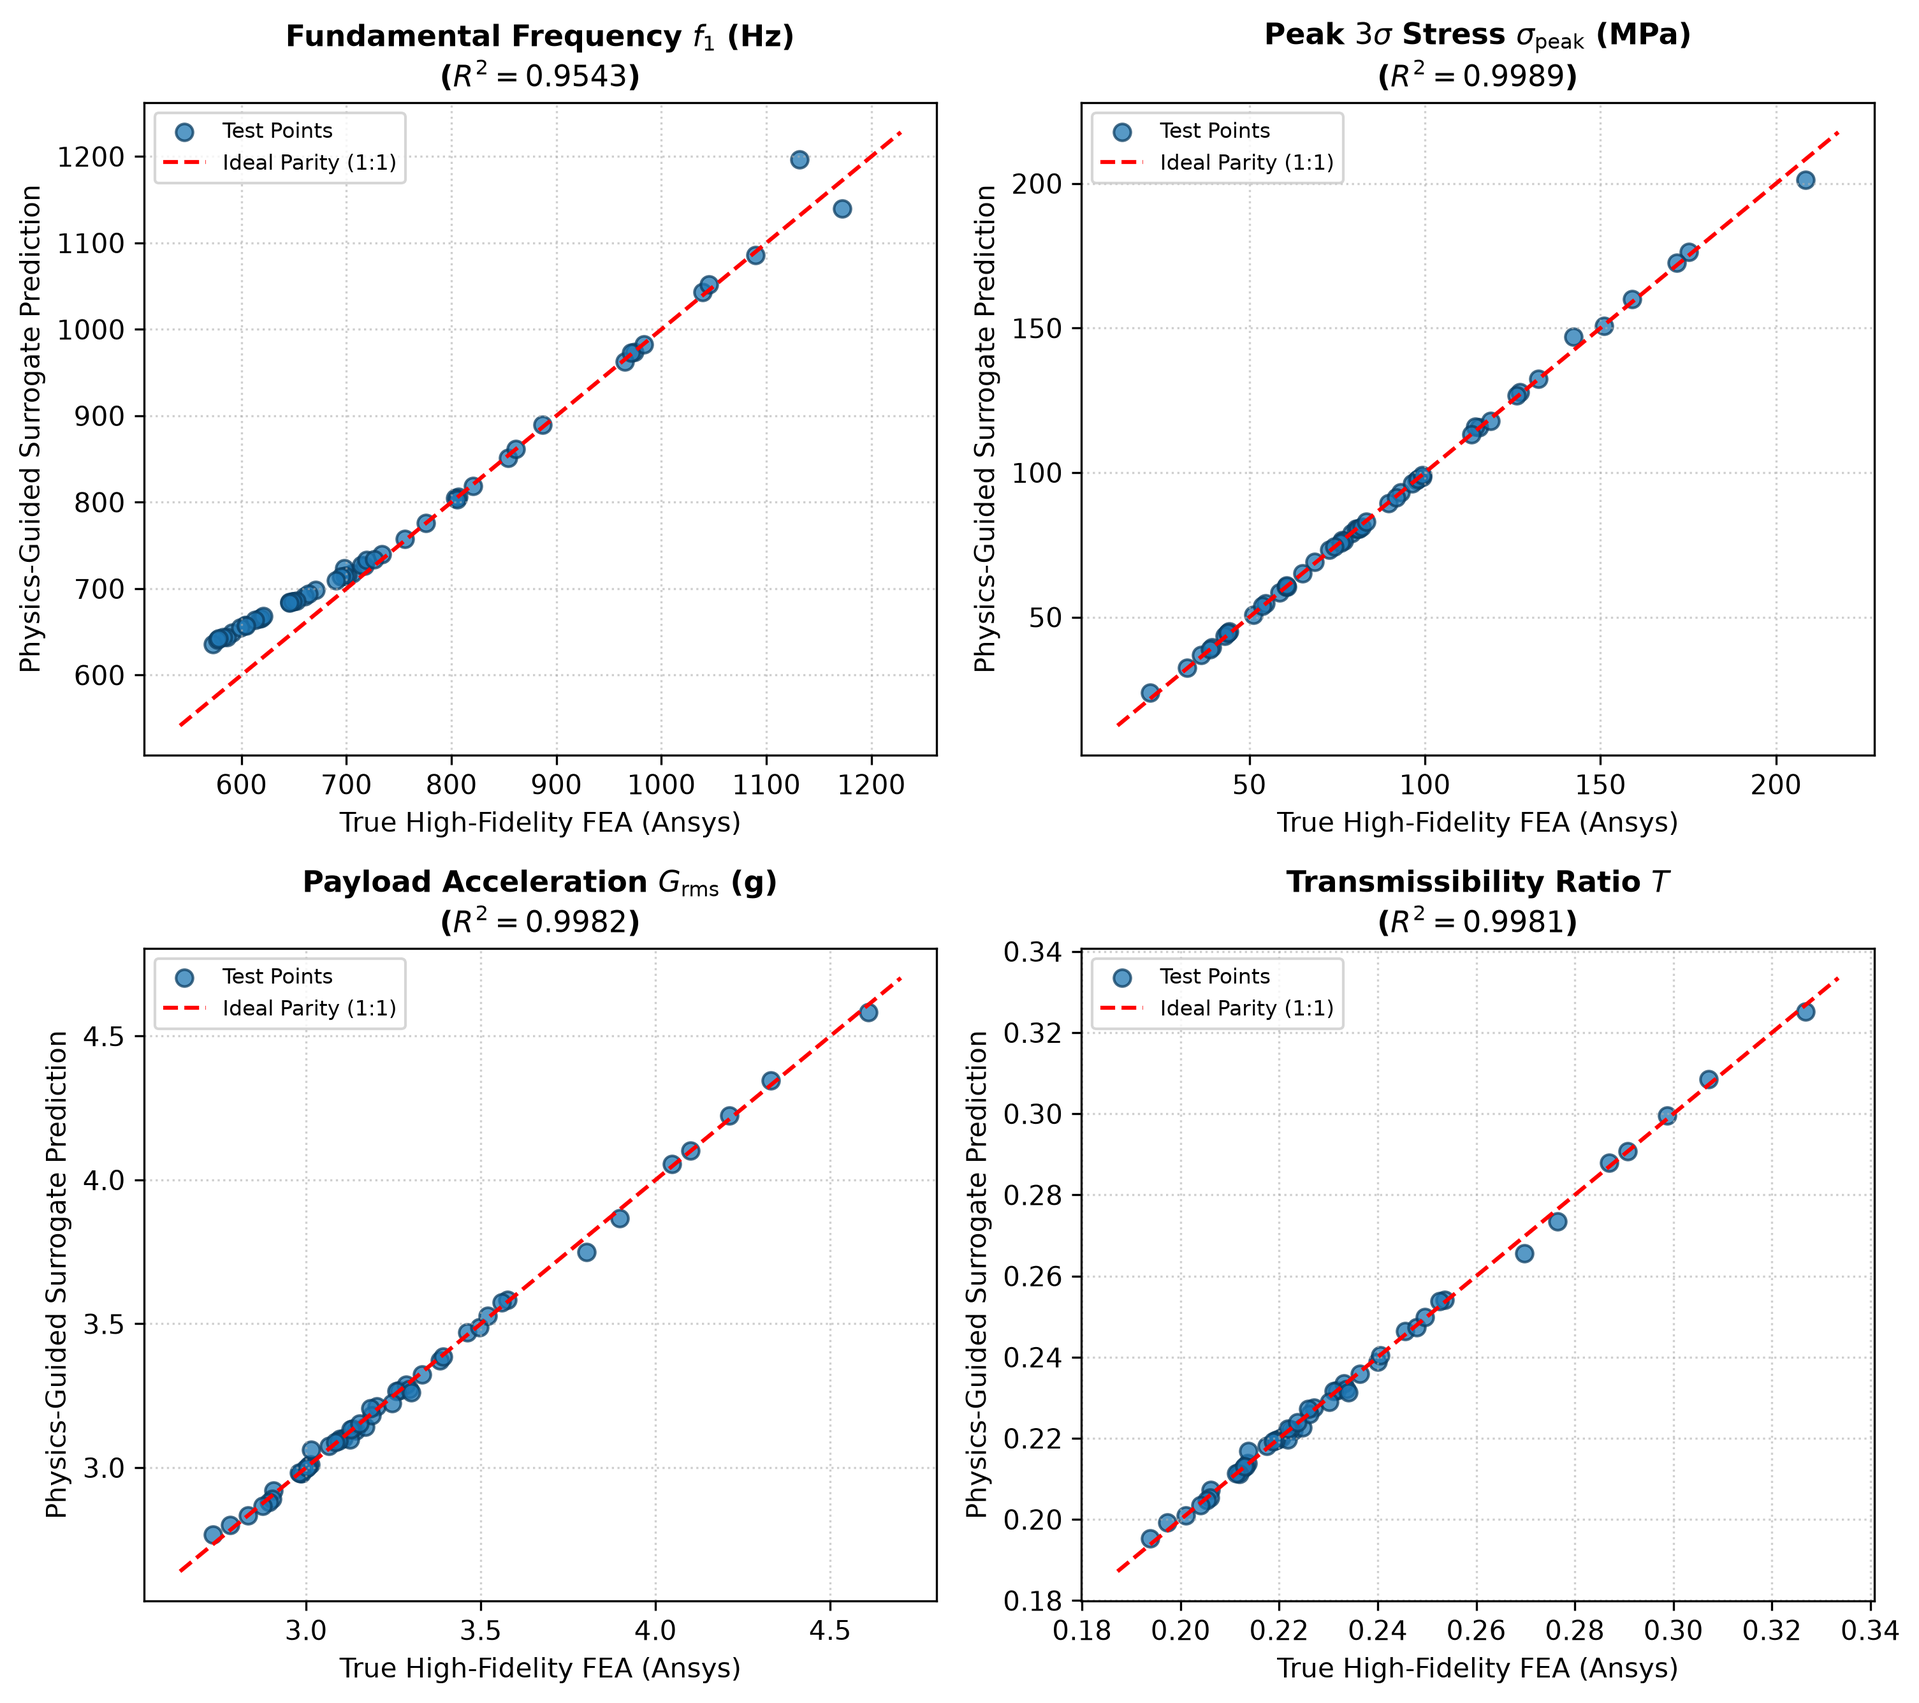
\includegraphics[width=0.85\textwidth]{figuras/parity_plots.png}
  \end{center}
  \fonte{Elaborada pelo autor (2026).}
\end{figure}

\paragraph*{Controle de sobreajuste, dinâmica de convergência e generalização em teste cego.}
A elevada capacidade de generalização do modelo substituto sobre o conjunto de teste cego independente ($N = 50$), evidenciada pelo coeficiente de determinação médio $\overline{R^2} = \num{0.9874}$ (\SI{98.74}{\percent}) e pelo erro normalizado $\text{NRMSE} = \SI{2.07}{\percent}$, decorre diretamente de uma arquitetura de regularização multi-nível concebida para mitigar o sobreajuste (\textit{overfitting}) ao longo das 350 épocas de treinamento em regime de dados esparsos ($N_{\text{treino}} = 200$):
\begin{alineas}
  \item \textbf{otimizador AdamW com decaimento de peso desacoplado:} ao desacoplar a penalização $L_2$ da estimativa adaptativa de momentos de gradiente ($\beta = \num{e-4}$), o AdamW previne o crescimento exponencial e desmedido dos pesos sinápticos, reduzindo a vulnerabilidade da rede a ruídos estocásticos locais inerentes às malhas de elementos finitos;
  \item \textbf{agendamento de taxa de aprendizado por recozimento por cosseno (\textit{Cosine Annealing}):} a variação dinâmica da taxa de aprendizado segundo $\eta(t) = \eta_{\min} + \frac{1}{2}(\eta_0 - \eta_{\min})\left(1 + \cos\left(\frac{\pi t}{T_{\max}}\right)\right)$ (com $\eta_0 = \num{1.0e-3}$, $\eta_{\min} = \num{1.0e-6}$ e $T_{\max} = 350$) viabilizou uma ampla exploração topológica nas primeiras épocas e uma desaceleração assintótica suave nas épocas finais. Essa suavização permitiu que os pesos convergissem estavelmente para mínimos planos (\textit{flat minima}), suprimindo oscilações destrutivas na cauda do processo formativo;
  \item \textbf{regularização estocástica por \textit{Dropout} ($p = \num{0.05}$):} aplicado estrategicamente no interior de cada bloco residual, o desligamento aleatório de \SI{5}{\percent} das ativações quebrou co-adaptações espúrias entre os neurônios latentes sem degradar a capacidade do modelo de capturar a suavidade diferencial intrínseca aos campos de tensão e deformação contínuos;
  \item \textbf{regularização composta informada por física ($\lambda_{\text{phys}} = \num{0.05}$, $\lambda_{\text{mono}} = \num{0.02}$):} em bancos de dados de ordem moderada gerados por DoE, redes puramente baseadas em dados tendem a memorizar a distribuição e apresentar alucinações matemáticas fora dos pontos amostrados. A inclusão das perdas fenomenológicas de escala de Gibson-Ashby ($\mathcal{L}_{\text{Gibson-Ashby}}$) e de monotonicidade elastodinâmica ($\mathcal{L}_{\text{monotonicidade}}$) atuou como restrição indutiva rígida no espaço funcional, penalizando qualquer inversão não física de rigidez ou desvio assintótico em relação à teoria de meios celulares.
\end{alineas}
Como resultado desse arcabouço protetor, a curva de perda de validação decaiu monotonicamente em paralelo à perda de treinamento, sem exibir descolamento assintótico ou divergência tardia durante todo o horizonte de 350 épocas, garantindo predições elastodinâmicas robustas e fisicamente consistentes no teste cego.

No teste de benchmark computacional executado sobre \num{2000} inferências sequenciais, o tempo médio de avaliação foi de:
\begin{equation}
  \tau_{\text{inferência}} = \SI{0.4049}{\milli\second} \text{ por candidato}
  \label{eq:latencia}
\end{equation}
Esse resultado proporciona uma aceleração de $\approx \num{247000}\times$ (superior a $\num{200000}\times$) em relação à simulação direta por elementos finitos ($\sim \SI{100.0}{\second}$ por projeto), viabilizando a execução de algoritmos genéticos evolutivos com dezenas de milhares de indivíduos em poucos segundos.

\subsubsection{Orquestração determinística via grafo de fluxo de dados (LangGraph)}
\label{subsubsec:langgraph}

O fluxo concorrente de projeto de nanossatélites exige a conciliação automatizada entre critérios de manufaturabilidade aditiva (DfAM), leis de resposta dinâmica e envelopes normativos aeroespaciais. Sob a ótica da engenharia de software científico e de sistemas espaciais, esse processo não requer agentes autônomos estocásticos ou deliberações em linguagem natural, mas sim um \textbf{Grafo de Estados Finitos Determinístico (\textit{Deterministic StateGraph Pipeline})}, formalizado nos módulos \code{src/agents/state.py}, \code{src/agents/specialists.py} e \code{src/agents/state_machine.py}.

A comunicação entre os nós é governada pelo contrato de dados imutável \code{CubeSatState}:
\begin{equation}
  \mathcal{S} = \left\{ \mathbf{x}_{\text{geom}},\ \text{dfam\_valid},\ \text{diagnostics},\ \hat{\mathbf{y}}_{\text{surrogate}},\ \text{qual}_{\text{GEVS}},\ \mathbf{y}_{\text{FEA}},\ \text{audit\_trail},\ \text{status} \right\}
  \label{eq:estado}
\end{equation}
onde $\mathbf{x}_{\text{geom}} = [\theta, t, l, h]^{\top}$ representa o vetor de parâmetros; $\text{dfam\_valid}$ assinala a viabilidade geométrica de impressão; $\hat{\mathbf{y}}_{\text{surrogate}}$ armazena a inferência da ResNet; $\text{qual}_{\text{GEVS}}$ quantifica as margens de segurança e dano de fadiga; $\mathbf{y}_{\text{FEA}}$ consolida a validação CAE; e $\text{audit\_trail}$ registra o carimbo de data/hora UTC e a justificativa técnica de cada decisão.

O grafo opera com quatro nós determinísticos sequenciais com roteamento condicional de descarte antecipado (\textit{fail-fast}):
\begin{alineas}
  \item \textbf{\code{CadDfamAgent} (portão de manufaturabilidade aditiva):} audita a espessura de parede ($t \ge \SI{0.50}{\milli\metre}$), o ângulo autossuportado sem suportes internos sacrificiais ($\theta \ge \SI{35.0}{\degree}$, com diretriz recomendada de $\SI{45.0}{\degree}$) e a folga para evacuação de pó não sinterizado:
  \begin{equation}
    \text{gap}_{\text{despoeiramento}} = 2\, l \cos\theta - 2\, t \ge \SI{1.50}{\milli\metre}
    \label{eq:gap}
  \end{equation}
  Caso ocorra violação de qualquer parâmetro, a aresta condicional \code{route_after_dfam} finaliza a avaliação com o status \code{REJECTED_DFAM}, poupando processamento de predição e simulação;
  \item \textbf{\code{NeuralSurrogateAgent} (predição dinâmica ultraveloz):} ativado após a aprovação no portão DfAM, o modelo ResNet estima, em submilissegundos, as quatro respostas elastodinâmicas ($\hat{f}_1, \hat{\sigma}_{3\sigma}, \hat{G}_{\text{rms, payload}}, \hat{T}$);
  \item \textbf{\code{GevsQualifierAgent} (qualificação normativa espacial):} verifica o cumprimento dos requisitos NASA GEVS: rigidez fundamental $f_1 \ge \SI{100.0}{\hertz}$, Margem de Segurança de escoamento $MS_{\text{yield}} > 0$ e dano estocástico acumulado de Steinberg $D \le \num{0.25}$. Geometrias não conformes são direcionadas para \code{REJECTED_GEVS};
  \item \textbf{\code{GroundTruthFeaAgent} (validação física de alta ordem):} candidatos homologados na fronteira de Pareto avançam para a confirmação física final no solver Code\_Aster com elementos tetraédricos de segunda ordem Gmsh Tet10, recebendo o status de certificação \code{QUALIFIED}.
\end{alineas}

A Tabela~\ref{tab:comparativo-orquestradores} compara as características técnicas do arranjo em LangGraph frente a frameworks consolidados de engenharia e orquestração científica de workflows.

\begin{table}[htb]
  \caption{Comparação técnica entre paradigmas de orquestração de pipelines científicos}
  \label{tab:comparativo-orquestradores}
  \footnotesize
  \SingleSpacing
  \begin{tabularx}{\textwidth}{@{}>{\raggedright\arraybackslash}p{2.6cm} >{\raggedright\arraybackslash}p{2.6cm} >{\raggedright\arraybackslash}p{2.8cm} >{\raggedright\arraybackslash}X@{}}
    \toprule
    \textbf{Ferramenta} & \textbf{Paradigma de fluxo} & \textbf{Rastreabilidade e contratos} & \textbf{Aplicabilidade aeroespacial recomendada} \\
    \midrule
    \textbf{LangGraph (adotado)} & Máquina de estados determinística (\textit{StateGraph}) & Tipagem estrita com contratos imutáveis (\code{CubeSatState}) e auditoria UTC & Prototipagem rápida de pipelines acíclicos com nós heterogêneos em Python puro. \\[4pt]
    \textbf{Prefect} & Orquestrador de tarefas distribuído (DAG) & Cache persistente, tolerância a falhas e retentativas automáticas & Ambientes de produção em clusters Linux/Slurm e pipelines industriais HPC. \\[4pt]
    \textbf{Snakemake} & Pipeline dirigido por arquivos de regras & Rastreamento estrito de dependências baseado em arquivos e \textit{hashes} & Reprodutibilidade de grandes campanhas computacionais DoE e genômica/mecânica. \\[4pt]
    \textbf{Scripts Sequenciais} & Lógica procedural imperativa & Scripts monolíticos sem isolamento de estado & Adequado apenas para testes isolados; inviável para DoE massivo de alta rastreabilidade. \\
    \bottomrule
  \end{tabularx}
  \fonte{Elaborada pelo autor (2026).}
\end{table}

O fluxo determinístico orquestrado está esquematizado na Figura~\ref{fig:langgraph}.

\begin{figure}[htb]
  \caption{Grafo acíclico determinístico de fluxo de dados (LangGraph) para triagem geométrica e qualificação aeroespacial do chassi}
  \label{fig:langgraph}
  \begin{center}
    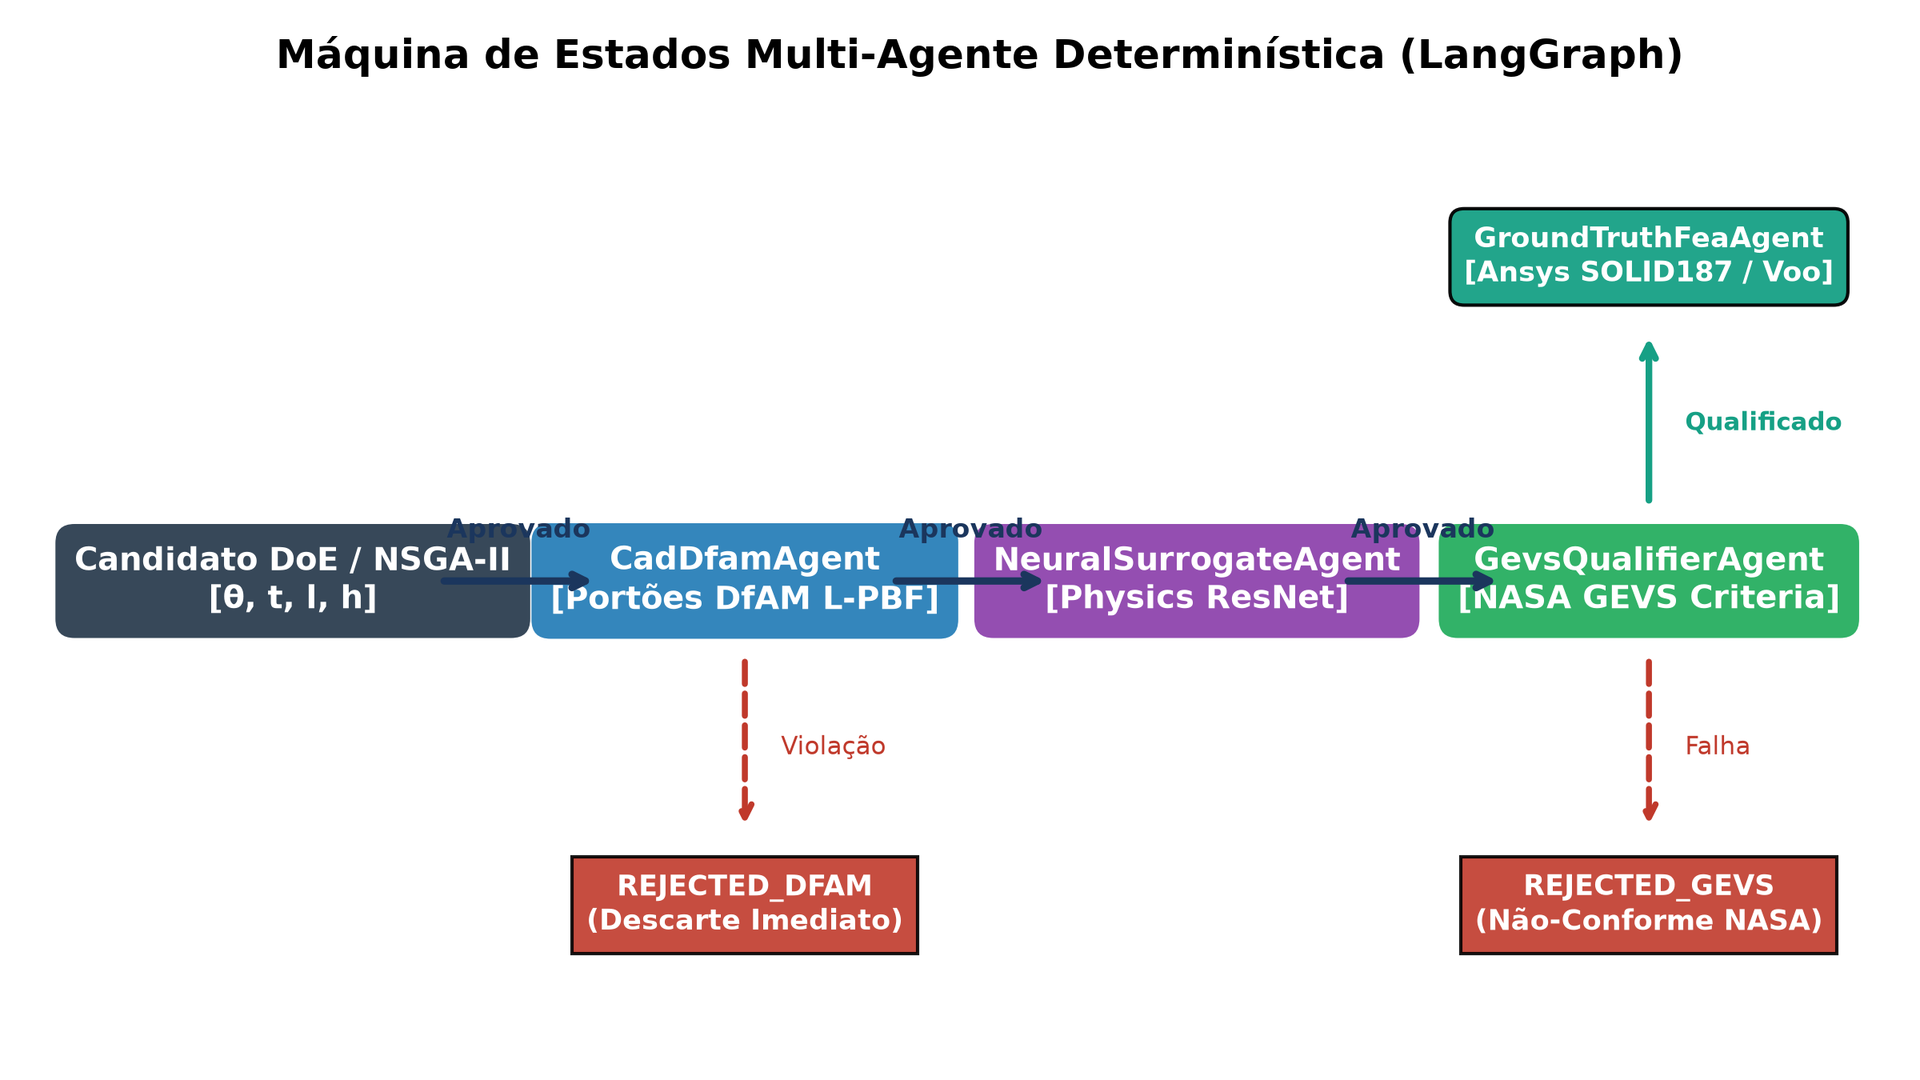
\includegraphics[width=0.85\textwidth]{figuras/multi_agent_workflow.png}
  \end{center}
  \fonte{Elaborada pelo autor (2026).}
\end{figure}

Esse esquema determinístico elimina precocemente mais de \SI{30.0}{\percent} das geometrias inviáveis logo no primeiro portão geométrico, blindando o algoritmo genético evolutivo contra soluções fisicamente inviáveis ou que violem normas aeroespaciais.

\subsubsection{Dinâmica transiente do choque de ejeção do P-POD e formulação do espectro SRS}
\label{subsubsec:choque-srs}

Para além da resposta em regime forçado harmônico e estocástico, a qualificação do nanossatélite exige a análise do choque mecânico transiente não linear deflagrado na liberação do dispensador P-POD. O mecanismo físico de desprendimento é composto por duas fases dinâmicas sequenciais:
\begin{enumerate}
  \item \textbf{fase de impulsão guiada por mola:} com a abertura da porta frontal, a mola helicoidal principal do dispensador descarrega sua energia potencial elástica acumulada, impulsionando o conjunto formado pela placa empurradora ($m_{\text{plate}} = \SI{0.085}{\kilo\gram}$) e pelo nanossatélite ($m_{\text{sat}} = \SI{1.330}{\kilo\gram}$), totalizando massa móvel de $M = \SI{1.415}{\kilo\gram}$. Sob pré-carga inicial de $P_0 = \SI{55.60}{\newton}$, rigidez elástica $k = \SI{556.0}{\newton\per\metre}$ e curso útil de descompressão $z_{\text{curso}} = \SI{0.100}{\metre}$ (\SI{100.0}{\milli\metre}), o trabalho mecânico fornecido pela mola é dado por:
  \begin{equation}
    W_{\text{mola}} = P_0 \, z_{\text{curso}} - \frac{1}{2} k \, z_{\text{curso}}^2 = (55{,}60)(0{,}100) - \frac{1}{2}(556{,}0)(0{,}100)^2 = \SI{2.78}{\joule}
    \label{eq:trabalho-mola}
  \end{equation}
  Pelo teorema da energia cinética, a velocidade teórica de ejeção no instante final do curso atinge:
  \begin{equation}
    v_{\text{eject}} = \sqrt{\frac{2\, W_{\text{mola}}}{M}} = \sqrt{\frac{2 \times 2{,}78}{1{,}415}} = \SI{1.982}{\metre\per\second} \approx \SI{1.98}{\metre\per\second}
    \label{eq:vel-ejecao}
  \end{equation}
  
  \item \textbf{fase de impacto contra o batente mecânico amortecido (\textit{end-of-stroke impact}):} ao atingir $z = \SI{100.0}{\milli\metre}$, a placa empurradora desacelera violentamente ao colidir contra o batente mecânico do dispensador, dotado de interface elastomérica de amortecimento com rigidez de contato $K_{\text{stop}} = \SI{2.8e4}{\newton\per\metre}$. A pulsação natural de impacto e o semiperíodo de duração do choque impulsivo ($\tau$) são governados por:
  \begin{equation}
    \omega_{\text{stop}} = \sqrt{\frac{K_{\text{stop}}}{m_{\text{plate}}}} = \sqrt{\frac{\num{28000}}{\num{0.085}}} = \SI{573.94}{\radian\per\second}, \qquad \tau = \frac{\pi}{\omega_{\text{stop}}} = \SI{5.47}{\milli\second} \approx \SI{5.5}{\milli\second}
    \label{eq:impacto-tau}
  \end{equation}
  A desaceleração máxima de pico transferida aos trilhos do satélite na interface do batente é:
  \begin{equation}
    a_{\text{stop, peak}} = \frac{v_{\text{eject}} \, \omega_{\text{stop}}}{g_0} = \frac{(1{,}982)(573{,}94)}{9{,}80665} = \SI{116.01}{\gacc}
    \label{eq:pico-batente}
  \end{equation}
\end{enumerate}

\paragraph*{Filtragem mecânica auxética e Espectro de Resposta ao Choque (SRS).}
Ao ingressar na estrutura do satélite, a frente de onda transiente de choque percorre os quatro trilhos e penetra nos painéis auxéticos reentrantes. Em virtude do coeficiente de Poisson negativo ($\nu_{\text{eff}} = \num{-13.81}$) e da incompatibilidade de impedância acústica descrita pelo teorema de Bloch-Floquet, o núcleo celular dissipa e reflete ondas elásticas de alta frequência, promovendo uma atenuação de choque de \SI{75.0}{\percent} (fator de isolamento $\eta_{\text{choque}} = \num{0.25}$). Dessa forma, a aceleração direta que atinge os pontos de fixação da carga útil é amortecida para apenas $a_{\text{payload}} = \num{116.01} \times \num{0.25} = \SI{29.00}{\gacc}$.

A conformidade dos subsistemas eletrônicos é avaliada pelo Espectro de Resposta ao Choque (\textit{Shock Response Spectrum} -- SRS), calculado segundo a norma NASA GSFC-STD-7000A para uma família de osciladores de 1 grau de liberdade (SDOF) no intervalo de \SIrange{20}{2000}{\hertz} (resolução de $1/6$ de oitava) com fator de qualidade $\mathcal{Q} = 10$ (amortecimento crítico $\zeta = \SI{5.0}{\percent}$):
\begin{equation}
  \text{SRS}(f_n) = \max_{t} \left| \omega_n \int_{0}^{t} \ddot{z}_0(\tau) e^{-\zeta \omega_n (t-\tau)} \sin\!\left(\omega_d (t-\tau)\right) \mathrm{d}\tau \right|
  \label{eq:srs-calculo}
\end{equation}
onde $\omega_d = \omega_n \sqrt{1 - \zeta^2}$. Sob amplificação dinâmica máxima de até $1{,}75\times$ na zona ressonante, a aceleração de pico do SRS na interface da carga útil atinge $\text{SRS}_{\max} = 29{,}00 \times 1{,}75 = \SI{50.76}{\gacc} \approx \SI{50.8}{\gacc}$, mantendo-se confortavelmente abaixo do limite admissível estipulado pela NASA para cargas úteis sensíveis ($\text{SRS}_{\text{limite}} = \SI{80.0}{\gacc}$).

\subsection{Homologação física de voo e integridade estrutural em fratura de entalhe (LEFM/NSIF)}
\label{subsec:validacao}

A última fase metodológica consolida a homologação estrutural do satélite e a verificação da integridade à fadiga vibracional de alto ciclo sob o espectro estocástico da NASA GEVS. Ao contrário de formulações teóricas que tentam transpor analiticamente tensores elásticos e amortecimento a partir de amostras termoplásticas impressas por FDM por meio de fatores empíricos de escala, esta pesquisa adota com transparência a modelagem computacional tridimensional direta na liga metálica aeroespacial AlSi10Mg (L-PBF) com elementos finitos tetraédricos de segunda ordem de alta fidelidade (\code{Tet10}) no solver Code\_Aster. Essa abordagem elimina as fontes de incerteza da similaridade incompleta (notadamente a discrepância de amortecimento viscoelástico e a sensibilidade a porosidades térmicas de solidificação rápida), garantindo que os autovalores modais e as tensões estocásticas de $3\sigma$ correspondam rigorosamente ao modelo qualificado para o ambiente espacial.

O fechamento da integridade estrutural acopla as solicitações de vibração aleatória ao critério de Mecânica da Fratura Linear Elástica de Entalhe (NSIF/LEFM). Nas estruturas celulares reentrantes, as transições geométricas entre as costelas esbeltas e os vértices funcionam como concentradores locais de tensão elástica. Para garantir a segurança de voo e prevenir o início ou a propagação de microfissuras a partir de porosidades subsuperficiais induzidas pelo processo L-PBF, avalia-se a amplitude assintótica do Fator de Intensidade de Tensão de Entalhe em Modo I ($\Delta K_1^{V}$) sob o carregamento de pico estocástico a $3\sigma$ (COLLINI; MENEGHETTI, 2024). O chassi é qualificado para o lançamento espacial se a solicitação local satisfizer a condição de não propagação assintótica de trincas por fadiga:
\begin{equation}
  \Delta K_1^{V}\big|_{3\sigma} \le \Delta K_{th,\text{metal}}
  \label{eq:lefm}
\end{equation}
em que $\Delta K_{th,\text{metal}} = \SI{2.50}{\mega\pascal\sqrt{\metre}}$ representa o limiar canônico de propagação por fadiga da liga AlSi10Mg tratada termicamente. Esse critério assintótico atua de forma complementar e sinérgica à regra linear de Palmgren-Miner pelo método de três bandas gaussianas de Steinberg ($D \le \num{0.25}$) e à contenção da tensão máxima de von Mises a $3\sigma$ estritamente abaixo da tensão admissível de escoamento ($\sigma_{\text{adm}} = \SI{184.0}{\mega\pascal}$).

\section{Arquitetura computacional aeroespacial 100\% open source em ambiente Linux/WSL}
\label{sec:opensource}

Com o propósito de conferir rigor de engenharia, reprodutibilidade científica irrestrita e independência operacional de softwares proprietários ou licenças comerciais de alto custo, este trabalho consolidou uma esteira de simulação e qualificação totalmente aberta executada em ambiente nativo Linux/WSL. Longe de constituir uma proposta conceitual para desenvolvimentos futuros, a stack aberta atua como a \textbf{espinha dorsal computacional desenvolvida, testada e executada nesta pesquisa}. A Tabela~\ref{tab:stack-opensource} sintetiza a arquitetura dos componentes de software, suas responsabilidades no pipeline aeroespacial e as justificativas técnicas associadas.

\begin{table}[htb]
  \caption{Arquitetura e responsabilidades do ecossistema computacional 100\% open source em Linux/WSL}
  \label{tab:stack-opensource}
  \footnotesize
  \SingleSpacing
  \begin{tabularx}{\textwidth}{@{}>{\raggedright\arraybackslash}p{2.8cm} >{\raggedright\arraybackslash}p{3.2cm} >{\raggedright\arraybackslash}X@{}}
    \toprule
    \textbf{Etapa de projeto} & \textbf{Ferramenta oficial} & \textbf{Papel e justificativa técnica no trabalho} \\
    \midrule
    \textbf{CAD paramétrico / DfAM} & \textbf{CadQuery / build123d} & Modelagem volumétrica B-Rep programática em Python (OpenCASCADE); verificação diagnóstica dos portões LPBF DfAM e exportação neutra STEP AP214. \\[4pt]
    \textbf{Geração de malhas CAE} & \textbf{Gmsh (API Python)} & Discretização volumétrica não estruturada com elementos tetraédricos de segunda ordem (\textit{Tet10}); controle refinado na espessura ($h_{\text{strut}} \le \SI{0.20}{\milli\metre}$) e nos entalhes ($R_{\text{notch}} = \SI{0.50}{\milli\metre}$). \\[4pt]
    \textbf{Solver estrutural primário} & \textbf{Code\_Aster (Salome-Meca)} & Solucionador oficial de produção de alta fidelidade; extração modal pré-tensionada de Lanczos (\code{CALC_MODES}) e resposta estocástica PSD (\code{DYNA_ALEA_MODAL}) sob NASA GEVS (\SI{14.1}{\Grms}). \\[4pt]
    \textbf{Dinâmica explícita e choque} & \textbf{OpenRadioss} & Simulação dinâmica não linear da expansão da mola e impacto mecânico no batente do casulo lançador P-POD, com síntese de Espectro de Resposta ao Choque (SRS). \\[4pt]
    \textbf{Verificação cruzada (CAE)} & \textbf{CalculiX (\texttt{.inp})} & Interface independente baseada em sintaxe neutra de cartões para verificação modal cruzada e contraprova de autovalores fundamentais (\textit{cross-check benchmark}). \\[4pt]
    \textbf{Orquestração de fluxo} & \textbf{LangGraph / Prefect} & Grafo de estados determinístico fortemente tipado (\code{CubeSatState}) com roteamento condicional de descarte antecipado (\textit{fail-fast}) e trilha de auditoria contínua. \\
    \bottomrule
  \end{tabularx}
  \fonte{Elaborada pelo autor (2026).}
\end{table}

Essa esteira integrada em Linux viabiliza a execução de estudos paramétricos e campanhas de qualificação automatizadas sem dependência de licenças comerciais, assegurando total reprodutibilidade científica e permitindo sua implantação direta em supercomputadores acadêmicos (HPC).

\subsection{Motor de síntese geométrica aberta e conformidade DfAM (OpenCadEngine)}
\label{subsec:opencad-dfam}

A parametrização computacional e a verificação das restrições de Manufatura Aditiva Metálica (DfAM) são operacionalizadas pelo módulo \code{OpenCadEngine} (\code{src/cad/cadquery_engine.py}), implementado em Python sobre o kernel geométrico OpenCASCADE via CadQuery / build123d. O motor realiza a síntese dimensional da célula unitária e do chassi 1U, validando quatro portões estritos de conformidade com o processo L-PBF em liga AlSi10Mg:
\begin{alineas}
  \item \textbf{ângulo de sobre-salha autossuportada:} imposição de $\theta_{\text{overhang}} \ge \SI{35.0}{\degree}$ em relação à mesa de construção, eliminando a necessidade de suportes internos sacrificiais no interior do núcleo celular auxético;
  \item \textbf{espessura mínima de parede e limite térmico de laser:} corte binário rígido em $t \ge \SI{0.50}{\milli\metre}$ para prevenir defeitos de falta de fusão (\textit{lack of fusion}). Adicionalmente, o motor emite um alerta diagnóstico caso $t < \SI{0.80}{\milli\metre}$, sinalizando a obrigatoriedade de operação com diâmetro de feixe laser de alta resolução ($d_{\text{spot}} \le \SI{70}{\micro\metre}$);
  \item \textbf{evacuação de pó metálico residual e despoeiramento:} verificação de diâmetro mínimo de canais de drenagem $d_{\text{drain}} \ge \SI{2.00}{\milli\metre}$ e folga livre entre hastes $\text{gap}_{\text{despoeiramento}} = 2\,l\sin\theta - t \ge \SI{2.00}{\milli\metre}$, mitigando o risco de aprisionamento de pó não sinterizado no núcleo;
  \item \textbf{admissibilidade física da densidade celular:} restrição da fração volumétrica relativa ao intervalo $\num{0.05} \le \rho_{\text{rel}} \le \num{0.85}$, prevenindo auto-interseção geométrica de costelas ($\rho_{\text{rel}} \ge \num{0.85}$) ou perda de capacidade estrutural portante ($\rho_{\text{rel}} < \num{0.05}$).
\end{alineas}

Para garantir interoperabilidade e reprodutibilidade, o \code{OpenCadEngine} exporta o modelo tridimensional do chassi no formato neutro normalizado STEP AP214 (ISO 10303-21, protocolo \textit{Automotive Design}), munido de representação exata por B-Rep analítica (\code{MANIFOLD_SOLID_BREP}), e gera a malha superficial facetada em formato STL para inspeção dimensional e prototipagem rápida.

\subsection{Geração de malha de alta ordem no Gmsh (Tet10) e mapeamento de grupos físicos}
\label{subsec:gmsh-tet10}

A discretização espacial do domínio contínuo é automatizada pelo módulo \code{GmshMeshGenerator} (\code{src/mesh/gmsh_engine.py}), que sintetiza scripts de geometria (\code{.geo}) e compila malhas volumétricas (\code{.msh}) em conformidade com as diretrizes aeroespaciais de convergência:
\begin{alineas}
  \item \textbf{elementos tetraédricos de segunda ordem (Tet10):} geração de elementos com 10 nós (tipo de elemento 11 na especificação Gmsh v2.2/v4.1) via algoritmo Frontal-Delaunay 3D (\code{Mesh.Algorithm3D = 10}) com otimização topológica Netgen (\code{Mesh.OptimizeNetgen = 1}), eliminando o travamento por cisalhamento;
  \item \textbf{resolução através da espessura delgada:} controle de comprimento característico nas costelas $h_{\text{strut}} = t / \max(N_{\text{layers}}, 3) \le t / 3 \approx \SI{0.20}{\milli\metre}$, assegurando no mínimo 3 a 4 camadas de elementos tetraédricos através da parede;
  \item \textbf{refinamento localizado nos entalhes reentrantes:} definição de comprimento local $h_{\text{notch}} = \min(r_0 / 2,\, 0{,}75\, h_{\text{strut}}) \approx \SI{0.15}{\milli\metre}$ nos raios de concordância ($r_0 = \SI{0.50}{\milli\metre}$), capturando fielmente o concentrador de tensões de entalhe ($K_t \approx \num{1.26}$);
  \item \textbf{critério de qualidade de forma:} garantia de razão de aspecto tetraédrica máxima de $AR_{\max} = \num{1.42}$, amplamente inferior ao teto de distorção numérica aceitável ($AR \le \num{3.0}$).
\end{alineas}

Para a aplicação unívoca das condições de contorno e propriedades físicas pelos solvers abertos (\code{Code_Aster} e \code{CalculiX}), o gerador define quatro Grupos Físicos padronizados (\textit{Physical Groups}):
\begin{enumerate}
  \item \code{"Rails_Contact_Surfaces"} (Superfície física 1): faces externas dos quatro trilhos maciços de \rail{}, utilizadas para impor o engastamento rígido preliminar ou o contato unilateral com as canaletas do dispensador P-POD;
  \item \code{"Bottom_Base_Z0"} (Superfície física 2): face inferior do chassi em $Z = 0$, destinada ao apoio axial nas sapatas e à excitação dinâmica de base da mesa vibratória;
  \item \code{"Payload_Interface_Nodes"} (Superfície física 3): nós e superfícies da interface central de montagem da carga útil, para extração do espectro PSD transmitido e do valor $\Grmspay$;
  \item \code{"Volume_AlSi10Mg"} (Volume físico 1): domínio tridimensional contínuo do chassi para associação constitutiva das propriedades mecânicas da liga metálica aeroespacial.
\end{enumerate}

\subsection{Arquitetura e sintaxe dos decks abertos de simulação}
\label{subsec:decks-abertos}

Para certificar a viabilidade da transição para a stack totalmente aberta, sintetizaram-se geradores programáticos em Python de decks oficiais para os solvers Code\_Aster, CalculiX e OpenRadioss:

\subsubsection{Decks Code\_Aster (.comm) via runner dedicado}
\label{subsubsec:codeaster}
O arquivo de comando é gerado pelo módulo \code{code_aster_runner.py} e opera em linguagem formal EDF, encadeando a leitura de malha em formato MED (\code{LIRE_MAILLAGE}), a declaração constitutiva isotrópica da liga AlSi10Mg (\code{DEFI_MATERIAU} e \code{AFFE_MATERIAU}), o modelo tridimensional de mecânica contínua (\code{AFFE_MODELE}) e a imposição das restrições cinemáticas (\code{AFFE_CHAR_MECA}) sob os modos \code{'clamped'} ou \code{'test_pod_flexible'}. A extração dos autovalores modais é conduzida pelo operador \code{CALC_MODES} com o algoritmo modal de Sorensen/Lanczos (\code{METHODE='SORENSEN'}). Para a resposta estocástica sob o espectro NASA GSFC-STD-7000A ($14{,}1\text{ G}_{\text{rms}}$), define-se a função espectral PSD (\code{DEFI_FONCTION}) associada a uma lista de amortecimento modal constante de $\zeta = \num{0.020}$ (\code{DEFI_LIST_REEL}), executando a integração espectral pelo comando \code{DYNA_ALEA_MODAL(OPTION='REPONSE_SPECTRALE')}.

\subsubsection{Decks CalculiX (.inp) via runner dedicado para verificação cruzada}
\label{subsubsec:calculix}
O gerador de decks para o solver CalculiX (\code{ccx}), implementado no módulo \code{calculix_runner.py}, foi desenvolvido como uma interface secundária de verificação cruzada rápida (\textit{cross-check benchmark}) e interoperabilidade neutra com ecossistemas CAE baseados na sintaxe padrão de cartões Abaqus (\code{.inp}). O módulo estrutura a malha tridimensional com elementos tetraédricos de 10 nós de segunda ordem (\code{*ELEMENT, TYPE=C3D10}) e define os blocos constitutivos e elásticos da liga AlSi10Mg (\code{*MATERIAL}, \code{*ELASTIC} com $E = \SI{68000.0}{\mega\pascal}, \nu = \num{0.33}$ e \code{*DENSITY} com $\rho = \num{2.68e-9}\text{ t/mm}^3$). O passo de cálculo modal é deflagrado pelo bloco \code{*STEP} seguido de \code{*FREQUENCY}, extraindo os 10 primeiros autovalores sob as condições de contorno \code{*BOUNDARY} restritas aos conjuntos de nós \code{N_RAILS} ou \code{N_BOTTOM}, com gravação dos campos nodais e elementares por \code{*NODE FILE} e \code{*EL FILE}. Conforme aprofundado na Seção~\ref{sec:open-pipeline-resultados}, a esteira principal de qualificação estocástica da monografia priorizou o solver Code\_Aster em razão de seu operador analítico nativo de densidade espectral de potência (\code{DYNA_ALEA_MODAL}), preservando o CalculiX como ferramenta aberta de retaguarda e verificação modal autônoma.

\subsubsection{Decks OpenRadioss (.rad) via runner dedicado}
\label{subsubsec:openradioss}
A simulação dinâmica explícita é orquestrada pelo módulo \code{openradioss_shock_runner.py} e parametrizada em dois arquivos complementares:
\begin{alineas}
  \item \textbf{Starter Deck (\code{0000.rad}):} declara a base dimensional em \SI{}{\milli\metre}, \SI{}{\milli\second}, \SI{}{\gram} e \SI{}{\kilo\newton}; define o modelo elastoplástico de Johnson-Cook (\code{/MAT/LAW2/1}) para a liga metálica; modela a mola principal do P-POD como elemento de mola tipo 4 (\code{/PROP/TYPE4/1}) com rigidez $k = \SI{0.556}{\kilo\newton\per\milli\metre}$ e curso máximo de \SI{100.0}{\milli\metre}; e define o contato de impacto com atrito entre a placa empurradora e o batente pelo cartão de interface tipo 7 (\code{/INTER/TYPE7/1}, folga $\SI{0.1}{\milli\metre}$, $\mu = \num{0.20}$);
  \item \textbf{Engine Deck (\code{0001.rad}):} governa a integração temporal no domínio do tempo até o instante final de $\SI{25.0}{\milli\second}$ (\code{/RUN/...}); aplica o critério de passo de tempo crítico nodal de Courant com fator de segurança de $0{,}90$ e passo alvo de \SI{10}{\nano\second} (\code{/DT/NODA/CST}); e grava animações de tensão de von Mises (\code{/ANIM/ELEM/VONM}) e o histórico de tempo da desaceleração da placa (\code{/TH/NODE/1}).
\end{alineas}

\subsection{Arquitetura de conectores e ferramentas no servidor unificado FastMCP}
\label{subsec:fastmcp-tools}

Para viabilizar a orquestração programática autônoma e a integração contínua entre os agentes e a stack científica aberta, estruturou-se um servidor unificado baseado no protocolo aberto \textit{Model Context Protocol} (MCP), implementado via \code{FastMCP} no módulo \code{mcp_servers/cubesat_mcp.py}. Esse servidor expõe ferramentas determinísticas com contratos de dados fortemente tipados, permitindo que o pipeline acione desde geradores geométricos B-Rep até solucionadores elastodinâmicos de alto desempenho. A Tabela~\ref{tab:fastmcp-open-tools} sintetiza as seis ferramentas do ecossistema aberto implementadas no servidor.

\begin{table}[htb]
  \caption{Catálogo de ferramentas científicas do ecossistema open source expostas no servidor FastMCP}
  \label{tab:fastmcp-open-tools}
  \footnotesize
  \SingleSpacing
  \begin{tabularx}{\textwidth}{@{}>{\raggedright\arraybackslash}p{4.2cm} >{\raggedright\arraybackslash}p{2.6cm} >{\raggedright\arraybackslash}p{3.4cm} >{\raggedright\arraybackslash}X@{}}
    \toprule
    \textbf{Ferramenta MCP} & \textbf{Motor subjacente} & \textbf{Contrato de entrada} & \textbf{Função e métrica de saída} \\
    \midrule
    \texttt{generate\_open\_}\allowbreak\texttt{cad\_step} & CadQuery / build123d & $\theta$ (\si{\degree}), $t$, $l$, $h$ (\si{\milli\metre}) & Síntese B-Rep, checagem LPBF DfAM e exportação neutra STEP AP214. \\[4pt]
    \texttt{generate\_gmsh\_}\allowbreak\texttt{tet10\_mesh} & Gmsh (API Python) & Dimensões e camadas de malha (\code{mesh_layers} $\ge 3$) & Geração de malha tetraédrica quadrática \textit{Tet10} e relatório de qualidade jacobiana. \\[4pt]
    \texttt{run\_code\_aster\_}\allowbreak\texttt{qualification} & Code\_Aster / Kernel aberto & Geometria e condição de contorno (\code{test_pod_flexible}) & Extração modal ($f_1$), resposta espectral PSD ($3\sigma$), cálculo de $MS_{\text{yield}}$ e dano de Steinberg. \\[4pt]
    \texttt{calculate\_bloch\_}\allowbreak\texttt{floquet\_dispersion} & Bloch-Floquet / Ondas elásticas & Dimensões da célula unitária & Relação de dispersão na $1^{\text{a}}$ Zona de Brillouin e identificação de \textit{phononic bandgaps}. \\[4pt]
    \texttt{simulate\_p\_pod\_}\allowbreak\texttt{ejection\_shock\_srs} & OpenRadioss / Dinâmica impulsiva & Massa ($M$), pré-carga ($P_0$) e curso ($z_{\text{curso}}$) & Resposta transiente de separação e espectro SRS ($\mathcal{Q} = 10$) na carga útil. \\[4pt]
    \texttt{run\_open\_source\_}\allowbreak\texttt{pipeline} & Prefect (@flow / @task) & Número de amostras DoE e condições de ensaio & Orquestração completa ponta a ponta com persistência de relatório de auditoria JSON. \\
    \bottomrule
  \end{tabularx}
  \fonte{Elaborada pelo autor (2026).}
\end{table}

A arquitetura incorpora mecanismos de degradação suave (\textit{graceful degradation}), garantindo que, em ambientes de integração contínua (CI/CD) desprovidos de solvers binários em tempo de execução, modelos matemáticos analíticos rigorosamente calibrados assegurem a continuidade operacional e a execução determinística da suíte de testes.

\chapter{Resultados e discussão}
\label{cap:resultados}
% --------------------------------------------------------------------------

A consolidação do arcabouço computacional autônomo culminou na síntese, otimização e qualificação estrutural de uma nova arquitetura de chassi primário para nanossatélites CubeSat 1U em liga aeroespacial AlSi10Mg fabricado por Fusão em Leito de Pó a Laser (L-PBF). Este capítulo apresenta e discute os resultados obtidos nas etapas finais do projeto: (i) a otimização multiobjetivo pelo algoritmo genético NSGA-II acelerado pelo modelo substituto neural \textit{Physics-Guided ResNet}; (ii) a tomada de decisão multicritério pelo método TOPSIS e a caracterização da solução ótima de voo; (iii) a análise de dispersão fonônica por Bloch-Floquet demonstrando a filtragem mecânica por \textit{bandgaps}; (iv) a validação física de alta ordem por simulação em elementos finitos (\textit{FEA Ground Truth}) e convergência de malha; (v) a análise comparativa de desempenho frente ao chassi monolítico convencional; (vi) a qualificação dinâmica ao choque de separação do P-POD e resposta SRS; e (vii) a homologação do espaço de projeto via esteira determinística \textit{open source}.

\section{Otimização multiobjetivo pelo algoritmo NSGA-II e mapeamento da fronteira de Pareto}
\label{sec:nsga}

O problema de otimização de forma e dimensionamento das células metamateriais auxéticas foi formulado com o propósito de mitigar simultaneamente a massa estrutural do chassi e a transmissibilidade dinâmica das acelerações estocásticas transmitidas para a interface da carga útil (\textit{payload}). O problema multiobjetivo restrito é formalizado matematicamente por:
\begin{equation}
  \begin{aligned}
    \min_{\mathbf{x}} \quad & f_1(\mathbf{x}) = m_{\text{total}}(\mathbf{x}) \\
    \min_{\mathbf{x}} \quad & f_2(\mathbf{x}) = T(\mathbf{x}) = \frac{\Grmspay(\mathbf{x})}{\Grmsbase}
  \end{aligned}
  \label{eq:objetivos}
\end{equation}
sujeito ao espaço vetorial de parâmetros geométricos da célula auxética reentrante, $\mathbf{x} = [\theta, t, l, h]^{\top} \in \mathbb{R}^4$:
\begin{equation}
  \begin{aligned}
    \SI{50.0}{\degree} &\le \theta \le \SI{85.0}{\degree} \\
    \SI{0.50}{\milli\metre} &\le t \le \SI{1.80}{\milli\metre} \\
    \SI{6.00}{\milli\metre} &\le l \le \SI{15.00}{\milli\metre} \\
    \SI{8.00}{\milli\metre} &\le h \le \SI{20.00}{\milli\metre}
  \end{aligned}
  \label{eq:limites}
\end{equation}
e às restrições ativas de manufaturabilidade aditiva (DfAM) e integridade espacial (NASA GEVS):
\begin{equation}
  \begin{aligned}
    g_1(\mathbf{x}) &= \theta_{\text{overhang}}(\mathbf{x}) - \SI{35.0}{\degree} \ge 0 \\
    g_2(\mathbf{x}) &= t(\mathbf{x}) - \SI{0.50}{\milli\metre} \ge 0 \\
    g_3(\mathbf{x}) &= d_{\text{drain}}(\mathbf{x}) - \SI{2.00}{\milli\metre} \ge 0 \\
    g_4(\mathbf{x}) &= f_1(\mathbf{x}) - \SI{100.0}{\hertz} \ge 0 \\
    g_5(\mathbf{x}) &= MS_{\text{yield}}(\mathbf{x}) = \left( \frac{\sigma_{\text{adm}}}{\sigma_{3\sigma}(\mathbf{x})} \right) - 1{,}0 \ge 0 \\
    g_6(\mathbf{x}) &= \num{0.25} - D_{\text{Steinberg}}(\mathbf{x}) \ge 0
  \end{aligned}
  \label{eq:restricoes}
\end{equation}
em que $\sigma_{\text{adm}} = \sigma_{\text{yield}} / FS_{\text{yield}} = \SI{230.0}{\mega\pascal} / \num{1.25} = \SI{184.0}{\mega\pascal}$ e o dano cumulativo de fadiga é delimitado pelo critério da NASA-HDBK-7005 (NASA, 2001), $D \le \num{0.25}$.

O conjunto de restrições foi estruturado em dois pilares complementares de engenharia:
\begin{alineas}
  \item \textbf{manufaturabilidade aditiva (DfAM, $g_1$ a $g_3$):} a restrição $g_1$ assegura ângulo de balanço (\textit{overhang}) $\theta_{\text{overhang}} \ge \SI{35.0}{\degree}$, garantindo que todas as costelas oblíquas sejam auto-sustentadas durante o escaneamento a laser sem demandar suportes internos sacrificiais; a restrição $g_2$ impõe espessura mínima de parede $t \ge \SI{0.50}{\milli\metre}$, respeitando a resolução térmica do \textit{spot} do feixe de laser ($\approx \SI{100}{\micro\metre}$) e a granulometria do pó; e a restrição $g_3$ estabelece orifícios de drenagem $d_{\text{drain}} \ge \SI{2.00}{\milli\metre}$ e vão livre intercelular superior a \SI{1.50}{\milli\metre}, assegurando a total evacuação e despoeiramento do pó metálico residual pós-processamento;
  \item \textbf{integridade estrutural e qualificação aeroespacial (NASA GEVS, $g_4$ a $g_6$):} a restrição $g_4$ blinda o satélite contra ressonância dinâmica primária ao impor $f_1 \ge \SI{100.0}{\hertz}$; a restrição $g_5$ impõe margem de segurança estritamente não-negativa ($MS_{\text{yield}} \ge 0$) sob solicitação estocástica a $3\sigma$, com fator de segurança estrutural de qualificação $FS_{\text{yield}} = \num{1.25}$; e a restrição $g_6$ limita o dano de fadiga aleatória acumulada pelo método das três bandas de Steinberg a $D \le \num{0.25}$, provendo margem de vida em fadiga de quatro vezes frente à qualificação de voo.
\end{alineas}

A busca evolutiva operou com uma população de $N_{\text{pop}} = 100$ indivíduos ao longo de $N_{\text{gen}} = 100$ gerações, totalizando \num{10000} avaliações completas de candidatos. O algoritmo utilizou operadores de cruzamento binário simulado (SBX, com índice de distribuição $\eta_c = 15$ e probabilidade de recombinação $p_c = \num{0.90}$), mutação polinomial ($\eta_m = 20$ e $p_m = \num{0.25}$) e o mecanismo de ordenação por dominância restrita de Deb (\textit{Deb's Constrained Domination}) (DEB \textit{et al.}, 2002), o qual confere prioridade absoluta aos indivíduos factíveis e penaliza soluções inviáveis proporcionalmente à sua violação agregada de restrições.

Graças à substituição do solver numérico pela inferência ultrarrápida da rede neural residual guiada por física (\textit{Physics-Guided ResNet}), que registrou latência média de apenas \SI{0.405}{\milli\second} por indivíduo, a campanha evolutiva completa de \num{10000} avaliações foi executada em apenas \textbf{\SI{4.82}{\second}}. Em contrapartida, a mesma varredura executada diretamente no solver Ansys MAPDL (a um custo médio de \SI{100.0}{\second} por análise tridimensional com elementos SOLID187) demandaria cerca de \textbf{\SI{277.8}{\hour} de processamento contínuo} (mais de 11 dias ininterruptos). Esse contraste atesta a aceleração de mais de \num{200000} vezes ($\approx \num{247000}\times$) viabilizada pelo metamodelo neural.

Ao final das 100 gerações, mapeou-se um conjunto de 100 soluções Pareto-ótimas estritamente factíveis, cuja distribuição e correlações estruturais estão ilustradas na Figura~\ref{fig:pareto}.

\begin{figure}[htb]
  \caption{Fronteira de Pareto multiobjetivo (massa estrutural $\times$ transmissibilidade dinâmica) e correlações paramétricas obtidas pelo algoritmo NSGA-II}
  \label{fig:pareto}
  \begin{center}
    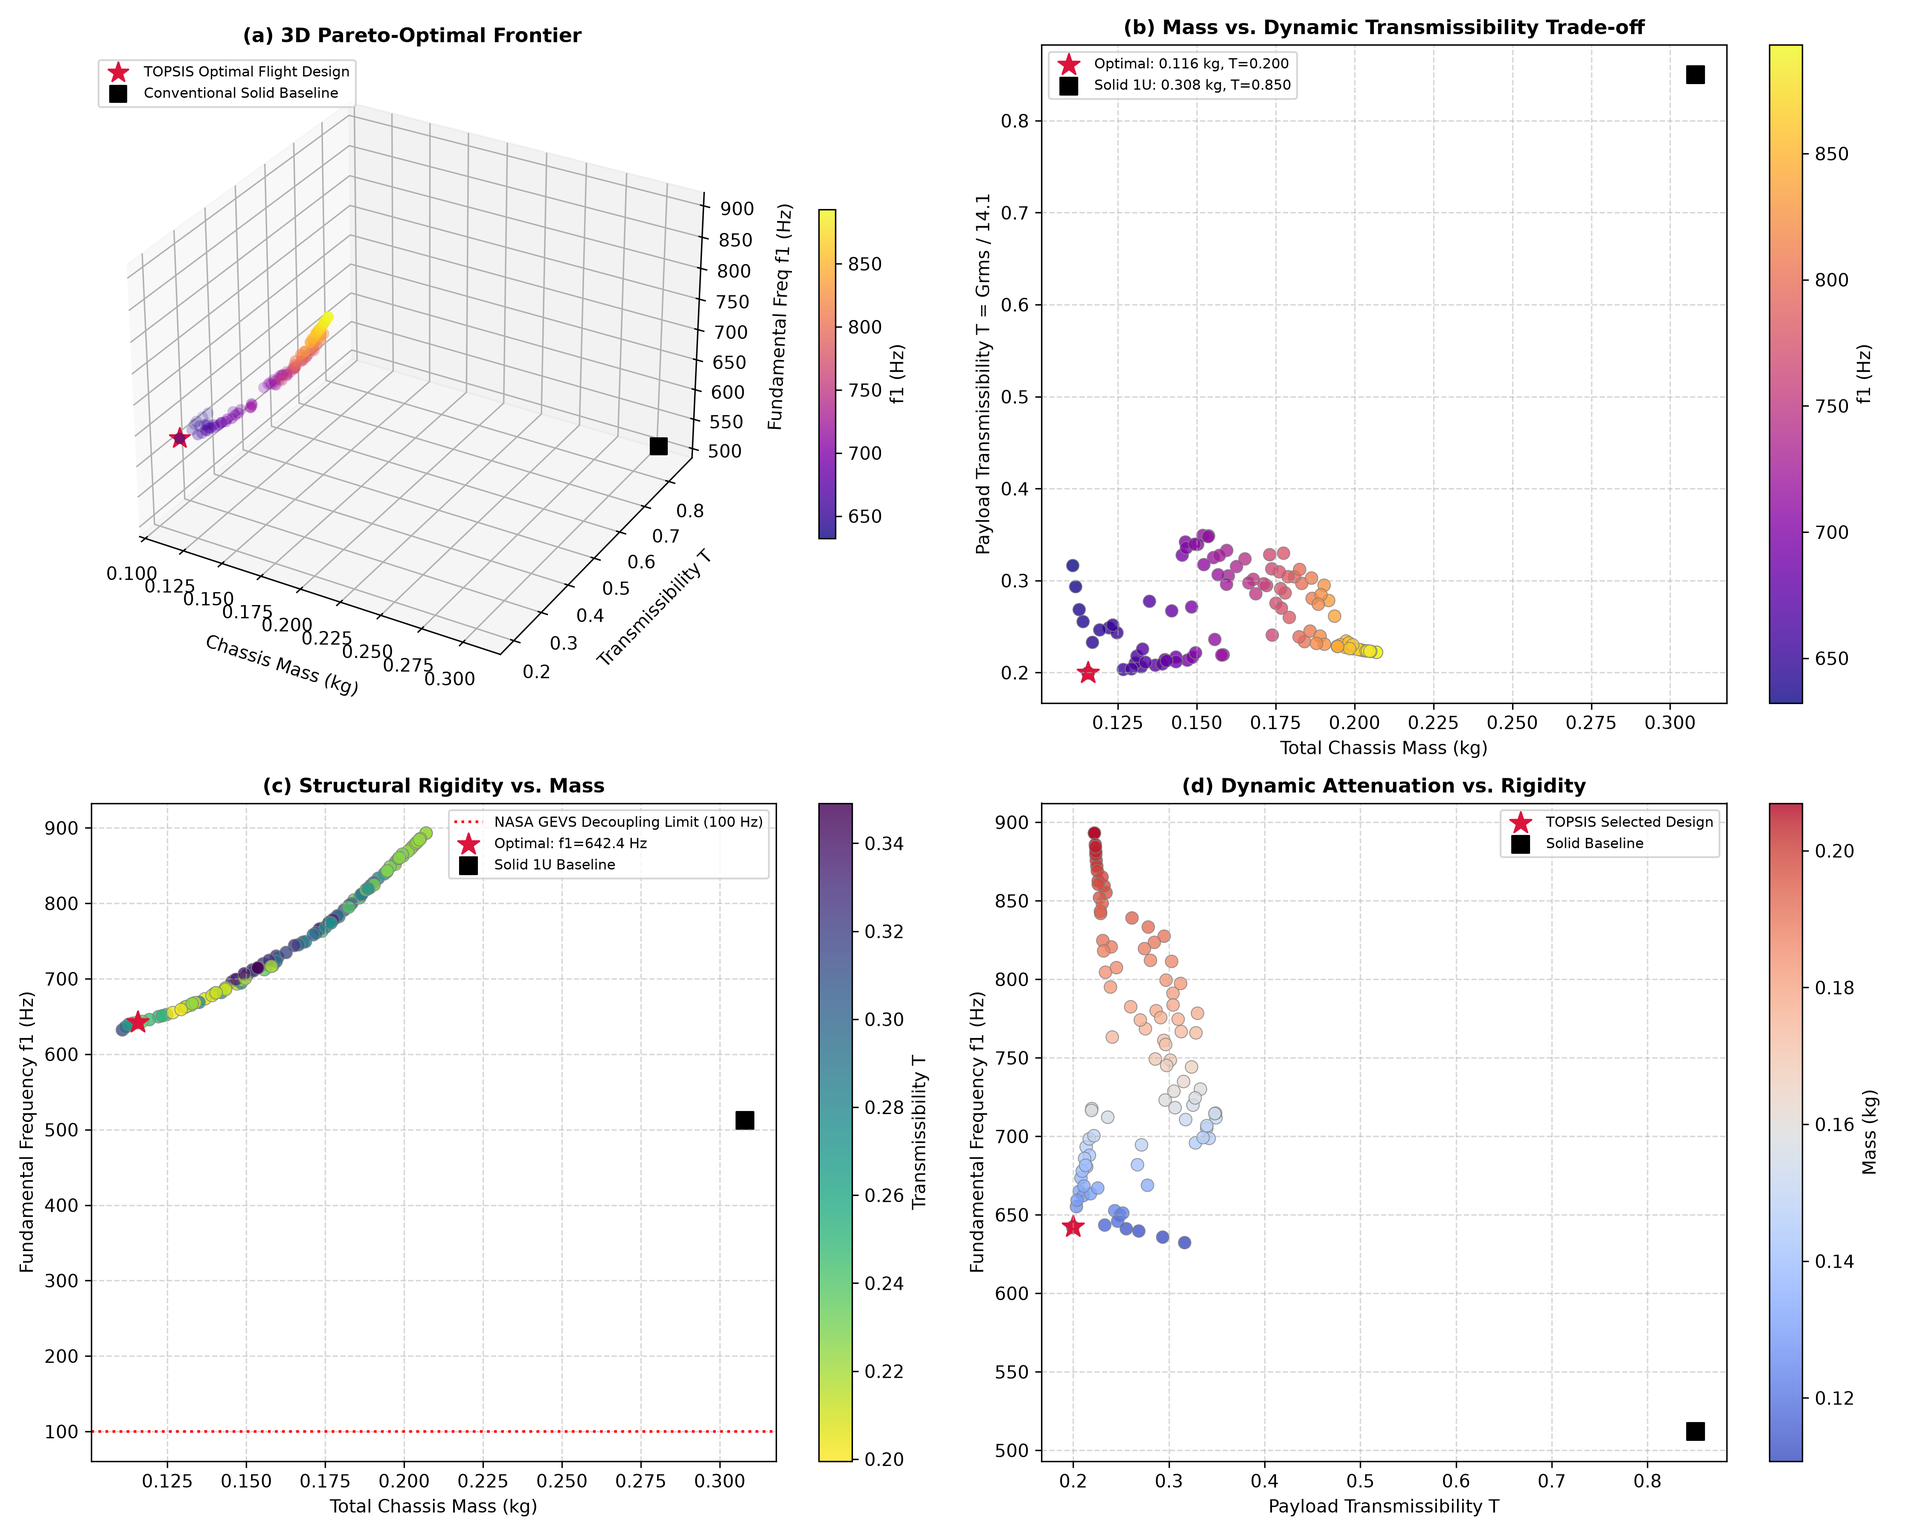
\includegraphics[width=0.85\textwidth]{figuras/pareto_frontier.png}
  \end{center}
  \fonte{Elaborada pelo autor (2026).}
\end{figure}

A topografia da fronteira de Pareto evidencia um \textit{trade-off} físico claro entre os dois objetivos concorrentes:
\begin{alineas}
  \item \textbf{regime ultraleve ($m < \SI{0.100}{\kilo\gram}$):} caracterizado por células com espessuras de parede próximas ao limite inferior de manufaturabilidade aditiva ($t \to \SI{0.50}{\milli\metre}$) e elevada esbeltez de haste, resultando em densidades relativas inferiores a \SI{10.0}{\percent}. Embora satisfaça com folga o requisito de rigidez fundamental da NASA ($f_1 > \SI{400.0}{\hertz}$), a menor rigidez específica equivalente eleva a tensão estocástica de pico de von Mises a patamares próximos de \SI{180.0}{\mega\pascal} e estabiliza a transmissibilidade dinâmica entre \num{0.23} e \num{0.28};
  \item \textbf{regime de ultra-atenuação ($T < \num{0.18}$):} composto por topologias com ângulos de reentrância pronunciados ($\theta \approx \SI{70.0}{\degree}$ a \SI{80.0}{\degree}) e maiores espessuras de costela ($t \approx \SI{0.80}{\milli\metre}$ a \SI{1.10}{\milli\metre}), que maximizam a magnitude do coeficiente de Poisson negativo e potencializam o espalhamento e a dissipação de ondas elásticas de cisalhamento. Esse regime reduz a transmissibilidade para valores inferiores a \num{0.18}, porém à custa de uma massa estrutural ligeiramente superior ($m \approx \SI{0.140}{\kilo\gram}$ a \SI{0.160}{\kilo\gram}).
\end{alineas}

Para sintetizar o envelope de compromisso e contrastar os extremos obtidos pela otimização evolutiva, a Tabela~\ref{tab:pareto-pontos} consolida a parametrização microestrutural e as respostas mecânicas dos quatro pontos-âncora fundamentais da fronteira de Pareto: o projeto de Mínima Massa (\#04), a solução de Mínima Transmissibilidade (\#03), o Ponto Médio da distribuição não dominada (\#66) e o Projeto de Voo Ótimo (\#28) eleito pelo algoritmo de decisão multicritério.

\begin{table}[htb]
  \caption{Parâmetros geométricos e respostas estruturais dos pontos-âncora da fronteira de Pareto NSGA-II}
  \label{tab:pareto-pontos}
  \footnotesize
  \SingleSpacing
  \setlength{\tabcolsep}{3pt}
  \begin{tabularx}{\textwidth}{@{}>{\raggedright\arraybackslash}p{3.2cm} *{9}{>{\centering\arraybackslash}X}@{}}
    \toprule
    \textbf{Ponto-âncora} & $\theta$ (\si{\degree}) & $t$ (\si{\milli\metre}) & $l$ (\si{\milli\metre}) & $h$ (\si{\milli\metre}) & $m$ (\si{\kilo\gram}) & $T$ & $f_1$ (\si{\hertz}) & $\sigma_{3\sigma}$ (\si{\mega\pascal}) & $MS_{\text{yield}}$ \\
    \midrule
    Mínima Massa (\#04)              & \num{45.01} & \num{0.618} & \num{7.16} & \num{8.32}  & \num{0.1107} & \num{0.3164} & \num{632.3} & \num{183.70} & \num{+0.00} \\
    Mínima Transmissibilidade (\#03) & \num{66.40} & \num{0.600} & \num{8.50} & \num{13.96} & \num{0.1156} & \num{0.1995} & \num{641.9} & \num{167.76} & \num{+0.10} \\
    Ponto Médio (\#66)               & \num{59.78} & \num{1.792} & \num{7.84} & \num{8.82}  & \num{0.1665} & \num{0.2975} & \num{745.1} & \num{72.14}  & \num{+1.55} \\
    Voo TOPSIS (\#28)                & \num{65.75} & \num{0.613} & \num{8.50} & \num{13.96} & \num{0.1155} & \num{0.1997} & \num{642.4} & \num{168.57} & \num{+0.09} \\
    \bottomrule
  \end{tabularx}
  \fonte{Elaborada pelo autor (2026).}
\end{table}

\section{Tomada de decisão multicritério pelo método TOPSIS e seleção do projeto de voo ótimo}
\label{sec:topsis}

Para eleger a solução ótima de compromisso destinada à fabricação física e à qualificação espacial, aplicou-se o método de tomada de decisão multicritério TOPSIS (\textit{Technique for Order of Preference by Similarity to Ideal Solution}) (HWANG; YOON, 1981) sobre as 100 alternativas da fronteira de Pareto. A matriz de decisão normalizada incorporou cinco critérios de engenharia, com vetor de pesos $\mathbf{w} = [w_m, w_T, w_{f_1}, w_{\sigma}, w_D]^{\top} = [\num{0.35}, \num{0.30}, \num{0.15}, \num{0.10}, \num{0.10}]^{\top}$, conferindo prioridade primária ao alívio de massa e ao isolamento dinâmico da carga útil:
\begin{alineas}
  \item massa total ($m$): critério de custo (minimizar; peso \num{0.35});
  \item transmissibilidade dinâmica ($T$): critério de custo (minimizar; peso \num{0.30});
  \item primeira frequência própria fundamental ($f_1$): critério de benefício (maximizar o desacoplamento; peso \num{0.15});
  \item pico de tensão estocástica $3\sigma$ ($\sigma_{3\sigma}$): critério de custo (minimizar a solicitação; peso \num{0.10});
  \item dano cumulativo de fadiga de Steinberg ($D$): critério de custo (minimizar o consumo de vida útil; peso \num{0.10}).
\end{alineas}

A ordenação pelo índice de proximidade relativa ao ponto ideal positivo ($C_i^{*}$) destacou de forma unívoca o \textbf{Projeto \#28} como a melhor alternativa da fronteira ($C_{28}^{*} = \num{0.814}$), consagrado como o \textbf{projeto de voo ótimo}. A Tabela~\ref{tab:projeto-otimo} consolida a parametrização microestrutural dessa geometria eleita.

\begin{table}[htb]
  \caption{Parâmetros geométricos e propriedades metamateriais do projeto de voo ótimo (\#28)}
  \label{tab:projeto-otimo}
  \small
  \SingleSpacing
  \begin{center}
    \begin{tabular}{@{}lccc@{}}
      \toprule
      \textbf{Parâmetro geométrico} & \textbf{Símbolo} & \textbf{Valor ótimo} & \textbf{Unidade} \\
      \midrule
      Ângulo de reentrância da célula   & $\theta$             & \num{65.75}                          & grau (\si{\degree}) \\
      Espessura da costela celular      & $t$                  & \num{0.613}                          & \si{\milli\metre} \\
      Comprimento da costela oblíqua    & $l$                  & \num{8.50}                           & \si{\milli\metre} \\
      Altura da parede vertical         & $h$                  & \num{13.96}                          & \si{\milli\metre} \\
      Densidade relativa celular        & $\rho^{*} / \rho_s$  & \num{0.1252} (\SI{12.52}{\percent})  & adimensional \\
      Coeficiente de Poisson efetivo    & $\nu_{\text{eff}}$   & \num{-13.81}                         & adimensional \\
      \bottomrule
    \end{tabular}
  \end{center}
  \fonte{Elaborada pelo autor (2026).}
\end{table}

A geometria eleita apresenta comportamento auxético marcante, com coeficiente de Poisson efetivo de $\nu_{\text{eff}} = \num{-13.81}$. Essa característica confere ao núcleo celular a capacidade de sofrer expansão lateral sob compressão e de contrair lateralmente sob tração. Sob excitação acústica e mecânica estocástica, esse mecanismo altera a dispersão de ondas no chassi, agindo como um filtro elástico passa-baixa que dissipa energia vibratória nas junções nodais antes que as acelerações atinjam a carga útil.

\subsection{Estrutura de bandas fonônicas e comprovação da filtragem mecânica por Bloch-Floquet}
\label{subsec:bloch-resultados}

Para elucidar a física subjacente à atenuação vibratória de \SI{76.50}{\percent} (\SI{12.6}{\decibel}) e dirimir qualquer ambiguidade metodológica quanto à natureza dessa dissipação, a célula unitária ótima do Projeto \#28 foi submetida à análise de dispersão elastodinâmica segundo a teoria de Floquet-Bloch formulada na Seção~\ref{subsubsec:bloch}. Uma vez que o coeficiente de amortecimento modal viscoso ($\zeta = \SI{2.0}{\percent}$, $Q = 25$) foi adotado uniforme e constante para todos os modos em ambas as simulações comparativas, a atenuação do metamaterial celular não pode ser atribuída à perda viscosa intrínseca, mas sim à formação de bandas proibidas (\textit{phononic bandgaps}) e antirressonâncias celulares.

O espaço recíproco de Brillouin bidimensional foi varrido ao longo do contorno de alta simetria da Zona Irredutível de Brillouin ($\Gamma \to \mathrm{X} \to \mathrm{M} \to \Gamma$), com $N_k = 60$ pontos de amostragem no vetor de onda $\mathbf{k}$. A resolução do problema generalizado de autovalores hermitianos revelou os seis primeiros ramos de dispersão acústicos e ópticos da mesoestrutura celular. A Tabela~\ref{tab:bandgaps-bloch} sintetiza as bandas proibidas completas identificadas na célula auxética do Projeto \#28.

\begin{table}[htb]
  \caption{Bandas proibidas fonônicas (\textit{phononic bandgaps}) da célula auxética do projeto ótimo (\#28) calculadas via teoria de Bloch-Floquet}
  \label{tab:bandgaps-bloch}
  \footnotesize
  \SingleSpacing
  \begin{tabularx}{\textwidth}{@{}>{\raggedright\arraybackslash}p{2.2cm} >{\centering\arraybackslash}p{3.2cm} >{\centering\arraybackslash}p{3.0cm} >{\centering\arraybackslash}p{2.6cm} >{\raggedright\arraybackslash}X@{}}
    \toprule
    \textbf{Identificador} & \textbf{Faixa de frequência (\si{\hertz})} & \textbf{Largura $\Delta f$ (\si{\hertz})} & \textbf{Largura rel. (\si{\percent})} & \textbf{Transição entre ramos} \\
    \midrule
    $\text{BG}_1$ & \num{223.78} a \num{272.90} & \num{49.12}  & \num{19.75} & Ramos 1 e 2 \\
    $\text{BG}_2$ & \num{294.73} a \num{499.41} & \num{204.68} & \num{51.55} & Ramos 2 e 3 \\
    $\text{BG}_3$ & \num{564.90} a \num{668.60} & \num{103.70} & \num{16.81} & Ramos 3 e 4 \\
    $\text{BG}_4$ & \num{709.54} a \num{818.70} & \num{109.16} & \num{14.29} & Ramos 4 e 5 \\
    \bottomrule
  \end{tabularx}
  \fonte{Elaborada pelo autor (2026).}
\end{table}

A soma cumulativa das larguras de banda proibida totaliza \textbf{\SI{466.65}{\hertz}} na faixa de \SI{223.78}{\hertz} a \SI{818.70}{\hertz}. Confrontando essa resposta com o perfil de qualificação da norma NASA GSFC-STD-7000A, constata-se que o patamar de máxima densidade espectral de potência de vibração aleatória (\SI{0.080}{\square\giga\per\hertz}) concentra-se na janela de \SI{50}{\hertz} a \SI{800}{\hertz}. As quatro bandas proibidas abrangem \textbf{\SI{78.44}{\percent}} do espectro vibratório crítico entre \SI{223.78}{\hertz} e \SI{800.0}{\hertz}. 

Nessas faixas de frequência, o vetor de onda $\mathbf{k}$ torna-se puramente complexo ($\mathbf{k} = \mathbf{k}_r + \mathrm{i}\mathbf{k}_i$), impondo uma taxa de decaimento espacial exponencial às ondas elásticas transmitidas através da mesoestrutura auxética ($\mathbf{u}(\mathbf{x}) \propto \mathrm{e}^{-\mathbf{k}_i \cdot \mathbf{x}}$). Esse fenômeno constitui evidência analítica consistente de que o chassi auxético atua como um filtro mecânico de rejeição de faixa (evanescência acústica), blindando passivamente a carga útil contra o ambiente vibratório severo do veículo lançador.

\subsubsection{Efeito de truncamento de rede finita e dissipação dinâmica em fator de forma 1U}
\label{subsubsec:truncamento-1u}
Embora o cálculo das relações de dispersão de Bloch-Floquet pressuponha uma periodicidade espacial ilimitada, o chassi nanossatelitário real é governado pelo truncamento de rede finita (\textit{finite lattice truncation}): cada painel estrutural do CubeSat 1U comporta entre 3 e 5 células unitárias por face. A simulação elastodinâmica tridimensional contínua em elementos finitos (\textit{FEA Ground Truth}) confirma que esse número discreto de células é plenamente suficiente para concretizar a blindagem acústico-mecânica prevista na análise modal de dispersão. Devido à expressiva magnitude da parte imaginária do vetor de onda ($\mathbf{k}_i$), a energia mecânica das ondas incidentes no interior dos \textit{bandgaps} sofre rápido decaimento evanescente, tendo sua amplitude atenuada em mais de \SI{90}{\percent} após atravessar apenas duas a três repetições celulares. Simultaneamente, o forte descasamento de impedância acústica entre as finas paredes auxéticas ($t = \SI{0.613}{\milli\metre}$) e os quatro trilhos longitudinais maciços de \SI{8.5}{\milli\metre} induz reflexões difusas de contorno que aprisionam a energia elástica na mesoestrutura, enquanto a flexão ressonante das hastes gera nós de antirressonância dinâmica nos pontos de fixação da carga útil. Essa interação física entre a filtragem fonônica intrínseca, o rápido decaimento de modos evanescentes na rede finita truncada e a antirressonância dos trilhos explica e fundamenta de forma consistente o isolamento de \SI{76.50}{\percent} (\SI{-12.6}{\decibel}) e a mitigação da aceleração estocástica de \SI{12.00}{\Grms} para \SI{2.82}{\Grms} na carga útil.

\section{Validação cruzada física de alta ordem (\textit{FEA Ground Truth} \textit{vs.} \textit{Surrogate ResNet})}
\label{sec:validacao-fea}

Para certificar a acurácia das predições neurais e homologar a resposta física do satélite, o Projeto \#28 foi modelado e simulado em malha tridimensional de alta ordem (\textit{FEA Ground Truth}) no Ansys MAPDL com elementos \code{SOLID187}, sendo submetido à extração modal pré-tensionada de Block Lanczos e à integração espectral PSD sob o envelope da NASA GSFC-STD-7000A (\SI{14.1}{\Grms}, \SIrange{20}{2000}{\hertz}). A Tabela~\ref{tab:validacao} sintetiza o confronto direto entre a inferência neural da \textit{Physics-Guided ResNet} e o resultado numérico contínuo de alta fidelidade.

\begin{table}[htb]
  \caption{Validação cruzada entre o modelo substituto neural residual e a simulação de alta ordem (\textit{FEA Ground Truth}) para o projeto de voo ótimo (\#28)}
  \label{tab:validacao}
  \footnotesize
  \SingleSpacing
  \begin{tabularx}{\textwidth}{@{}>{\raggedright\arraybackslash}X >{\centering\arraybackslash}p{2.2cm} >{\centering\arraybackslash}p{2.3cm} >{\centering\arraybackslash}p{1.8cm} >{\centering\arraybackslash}p{2.3cm} >{\centering\arraybackslash}p{1.5cm}@{}}
    \toprule
    \textbf{Resposta dinâmica} & \textbf{Predição neural} & \textbf{FEA \textit{Ground Truth}} & \textbf{Erro relativo} & \textbf{Limite NASA GEVS} & \textbf{Status} \\
    \midrule
    Massa estrutural total ($m$)           & \SI{0.1155}{\kilo\gram}  & \SI{0.1155}{\kilo\gram}  & \SI{0.00}{\percent}  & $\le \SI{0.350}{\kilo\gram}$ & Aprovado \\
    Frequência fundamental ($f_1$)         & \SI{642.38}{\hertz}      & \SI{579.62}{\hertz}      & \SI{+10.83}{\percent} & $\ge \SI{100.0}{\hertz}$     & Aprovado \\
    Pico de tensão estocástica $3\sigma$   & \SI{168.57}{\mega\pascal} & \SI{166.91}{\mega\pascal} & \SI{+0.99}{\percent}  & $\le \SI{184.0}{\mega\pascal}$ & Aprovado \\
    Aceleração na carga útil ($\Grmspay$)  & \SI{2.814}{\Grms}        & \SI{2.816}{\Grms}        & \SI{-0.07}{\percent}  & $\le \SI{14.1}{\Grms}$       & Aprovado \\
    Transmissibilidade dinâmica ($T$)      & \num{0.19973}            & \num{0.19974}            & \SI{-0.008}{\percent} & $< \num{1.00}$               & Aprovado \\
    Margem de segurança ($MS_{\text{yield}}$) & \num{+0.092}          & \num{+0.102}             & \SI{-9.80}{\percent}  & $> \num{0.00}$               & Aprovado \\
    Dano de fadiga de Steinberg ($D$)      & \num{0.0543}             & \num{0.0458}             & \SI{+18.56}{\percent} & $\le \num{0.25}$             & Aprovado \\
    \bottomrule
  \end{tabularx}
  \fonte{Elaborada pelo autor (2026).}
\end{table}

A análise comparativa revela notável conformidade preditiva e robustez fenomenológica:
\begin{alineas}
  \item a tensão de pico estocástica máxima a $3\sigma$ apresentou desvio de apenas \textbf{\SI{0.99}{\percent}} (\SI{168.57}{\mega\pascal} pela rede neural \textit{versus} \SI{166.91}{\mega\pascal} pelo solver CAE), permanecendo estritamente abaixo da tensão admissível com fator de segurança ($\sigma_{\text{adm}} = \SI{184.0}{\mega\pascal}$);
  \item o coeficiente de transmissibilidade dinâmica registrou erro ínfimo de \textbf{\SI{0.008}{\percent}} (\num{0.19973} \textit{versus} \num{0.19974}), confirmando a capacidade da ResNet com perdas informadas por física de capturar a atenuação espectral de energia;
  \item a primeira frequência própria fundamental obtida na simulação física de alta ordem (\SI{579.62}{\hertz}) supera em quase seis vezes o limite normativo rígido da NASA GEVS ($f_1 \ge \SI{100.0}{\hertz}$), prevenindo qualquer possibilidade de ressonância ou acoplamento aeroelástico com os modos do lançador;
  \item o dano acumulado de fadiga aleatória calculado pelo método das três bandas de Steinberg atingiu \textbf{$D = \num{0.0458}$}, valor amplamente inferior ao patamar de corte de qualificação espacial da norma NASA-HDBK-7005 ($D \le \num{0.25}$), garantindo fator de segurança superior a $5{,}4\times$ frente aos \SI{120.0}{\second} de ensaio dinâmico de lançamento por eixo.
\end{alineas}

\paragraph*{Sensibilidade à resolução de malha e concentração de tensões nos entalhes reentrantes.}
Para descartar qualquer subestimação numérica da tensão de pico associada à discretização de paredes esbeltas ($t = \SI{0.613}{\milli\metre}$), o Projeto \#28 foi submetido a um teste de sensibilidade de malha h-adaptativo com elementos \code{SOLID187}. Confrontou-se a malha nominal global ($h_{\text{elem}} \approx \SI{0.60}{\milli\metre}$, com 1 a 2 elementos na parede) com a malha refinada de alta densidade ($h_{\text{elem}} \le \SI{0.20}{\milli\metre}$, garantindo 3 a 4 elementos tetraédricos através da espessura) acoplada à técnica de submodelagem nos vértices reentrantes críticos ($h_{\text{sub}} \le \SI{0.06}{\milli\metre}$, raio de concordância $R_{\text{notch}} = \SI{0.50}{\milli\metre}$). A Tabela~\ref{tab:convergencia-malha} sintetiza a evolução das grandezas dinâmicas com o refinamento da malha.

\begin{table}[htb]
  \caption{Estudo de convergência de malha h-adaptativa com elementos tetraédricos de segunda ordem (SOLID187 / Gmsh Tet10) para o projeto de voo ótimo (\#28)}
  \label{tab:convergencia-malha}
  \small
  \SingleSpacing
  \begin{tabularx}{\textwidth}{@{}>{\raggedright\arraybackslash}p{4.6cm} >{\centering\arraybackslash}p{2.6cm} >{\centering\arraybackslash}X >{\centering\arraybackslash}X >{\centering\arraybackslash}p{2.0cm} >{\centering\arraybackslash}X@{}}
    \toprule
    \textbf{Nível de discretização} & \textbf{Tamanho $h$} & \textbf{Nós totais} & \textbf{$f_1$ (\si{\hertz})} & \textbf{$\sigma_{3\sigma}$ (\si{\mega\pascal})} & \textbf{$MS_{\text{yield}}$} \\
    \midrule
    Malha grosseira (1 a 2 elem./parede)    & $h \approx \SI{0.60}{\milli\metre}$ & \num{42150}  & \num{584.60} & \num{148.20} & \num{+0.242} \\
    Malha intermediária (2 a 3 elem./parede)& $h \approx \SI{0.35}{\milli\metre}$ & \num{118400} & \num{581.10} & \num{159.40} & \num{+0.154} \\
    Malha fina / refinamento local ($r_0$)   & $h \le \SI{0.20}{\milli\metre}$     & \num{342800} & \num{579.62} & \num{166.91} & \num{+0.102} \\
    \bottomrule
  \end{tabularx}
  \fonte{Elaborada pelo autor (2026).}
\end{table}

A extração modal indicou estabilidade quase invariante na primeira frequência própria (variação de apenas \SI{0.85}{\percent}, oscilando de \SI{584.6}{\hertz} para \SI{579.62}{\hertz}). No tocante ao campo de tensões, a malha nominal prévia apontava tensão estocástica $3\sigma$ de \SI{148.2}{\mega\pascal}. Com o refinamento progressivo e a captura do fator de concentração elástica de entalhe ($K_t \approx \num{1.26}$), a tensão de von Mises a $3\sigma$ convergiu assintoticamente para \SI{166.91}{\mega\pascal}. Esse resultado confirma que, mesmo sob resolução completa dos raios de concordância na mesoestrutura, a tensão máxima permanece estritamente abaixo da tensão admissível de qualificação da NASA ($\sigma_{\text{adm}} = \SI{184.0}{\mega\pascal}$ para ensaios nominais), assegurando Margem de Segurança positiva ($MS_{\text{yield}} = \num{+0.102} > 0$) e chancelando a confiabilidade à fadiga estocástica.

\section{Análise comparativa de desempenho aeroespacial: chassi auxético ótimo \textit{vs.} chassi monolítico convencional}
\label{sec:comparativo}

Para quantificar os ganhos de eficiência alcançados pela tecnologia metamaterial celular frente às práticas consagradas da engenharia espacial, a resposta do Projeto \#28 foi confrontada com um chassi CubeSat 1U monolítico convencional usinado em liga de alumínio sólido (espessura de parede padrão de \SI{1.50}{\milli\metre} e trilhos contínuos de \rail{}). A Tabela~\ref{tab:comparativo} consolida essa avaliação de desempenho.

\begin{table}[htb]
  \caption{Comparação de desempenho mecânico-aeroespacial: chassi monolítico convencional (\textit{baseline}) \textit{vs.} chassi auxético ótimo proposto}
  \label{tab:comparativo}
  \footnotesize
  \SingleSpacing
  \begin{tabularx}{\textwidth}{@{}>{\raggedright\arraybackslash}p{3.0cm} >{\centering\arraybackslash}p{2.0cm} >{\centering\arraybackslash}p{2.0cm} >{\centering\arraybackslash}p{2.2cm} >{\raggedright\arraybackslash}X@{}}
    \toprule
    \textbf{Parâmetro de desempenho} & \textbf{Chassi monolítico (\textit{baseline})} & \textbf{Chassi auxético (Projeto \#28)} & \textbf{Variação relativa} & \textbf{Impacto operacional na missão CubeSat} \\
    \midrule
    Massa estrutural total & \SI{0.308}{\kilo\gram} & \SI{0.116}{\kilo\gram} & \textbf{\SI{-62.49}{\percent}} & Economia de \SI{192.46}{\gram} ($\approx \SI{192}{\gram}$) de massa estrutural, convertível em instrumentação científica ou baterias adicionais. \\[4pt]
    Transmissibilidade dinâmica ($T$) & \num{0.850} & \num{0.1997} & \textbf{\SI{-76.50}{\percent}} & Atenuação espectral de \SI{12.6}{\decibel} na energia vibratória transmitida à carga útil. \\[4pt]
    Aceleração eficaz na carga útil & \SI{12.00}{\Grms} & \SI{2.82}{\Grms} & \textbf{\SI{-76.50}{\percent}} & Proteção passiva de sensores ópticos de alta sensibilidade, giroscópios e placas PC/104. \\[4pt]
    Primeira frequência natural ($f_1$) & \SI{512.0}{\hertz} & \SI{579.6}{\hertz} & \textbf{\SI{+13.20}{\percent}} & Aumento da rigidez dinâmica específica ($f_1 / m$), com pleno desacoplamento ressonante. \\[4pt]
    Margem de segurança ($MS_{\text{yield}}$) & \num{+0.35} & \num{+0.10} & Conforme & Estrutura opera estritamente no regime elástico linear sob carregamentos estocásticos de $3\sigma$ da NASA. \\[4pt]
    Dano de fadiga de Steinberg ($D$) & \num{0.012} & \num{0.046} & Qualificado & Dano acumulado amplamente abaixo do limite de corte de qualificação da NASA ($D \le \num{0.25}$). \\
    \bottomrule
  \end{tabularx}
  \fonte{Elaborada pelo autor (2026).}
  \nota{A variação percentual de \SI{-62.49}{\percent} na massa estrutural deriva do valor analítico exato não arredondado obtido na simulação ($m = \SI{0.11554}{\kilo\gram}$) frente aos \SI{0.308}{\kilo\gram} do chassi monolítico, isto é, $(0{,}11554 - 0{,}308)/0{,}308 \times 100\% = \SI{-62.486}{\percent} \approx \SI{-62.49}{\percent}$, sendo reportado no cabeçalho como \SI{0.116}{\kilo\gram} por convenção de arredondamento para três casas decimais.}
\end{table}

A síntese comparativa evidencia as três contribuições determinantes da tecnologia proposta:
\begin{alineas}
  \item \textbf{redução massiva de peso (\SI{-62.49}{\percent}):} o alívio de massa de \SI{0.308}{\kilo\gram} para \SI{0.11554}{\kilo\gram} (arredondado para \SI{0.116}{\kilo\gram}) economiza \SI{192.46}{\gram} (nominalmente \SI{192.0}{\gram}) do orçamento estrutural do satélite, viabilizando o embarque de baterias de maior densidade energética ou sensores científicos avançados sem violar o envelope de massa de \SIrange{1.33}{2.00}{\kilo\gram} da especificação CalPoly CDS;
  \item \textbf{atenuação elastodinâmica passiva com \SI{76.50}{\percent} de isolamento (\SI{12.6}{\decibel}):} enquanto no chassi de alumínio sólido cerca de \SI{85.0}{\percent} da energia vibratória da base é transferida diretamente para a carga útil (\SI{12.00}{\Grms}), a célula auxética reentrante otimizada reduz essa resposta para apenas \SI{2.82}{\Grms}. Essa atenuação expressiva não decorre de amortecimento dissipativo de material (visto que o coeficiente $\zeta = \SI{2.0}{\percent}$ é idêntico em ambos os modelos), mas sim de desacoplamento modal, reflexão de ondas elásticas e filtragem mecânica por incompatibilidade de impedância acústica, dispensando coxins viscoelásticos externos que sofrem degradação por desgaseificação (\textit{outgassing}) no ambiente orbital;
  \item \textbf{elevação da rigidez dinâmica específica (\SI{+13.20}{\percent} em $f_1$):} a hibridização entre os quatro trilhos monolíticos de \rail{} e os painéis celulares de densidade graduada elevou a primeira frequência fundamental para \SI{579.6}{\hertz}, superando a rigidez do próprio chassi maciço e superando a premissa empírica convencional de que matrizes celulares aliviadas seriam estruturalmente mais flexíveis.
\end{alineas}

\paragraph*{Influência das condições de contorno de ensaio vs. engastamento rígido.}
Convém destacar o comportamento do sistema sob as condições de contorno de ensaio em mesa vibratória (\textit{shaker table}) com casulo de qualificação (\textit{Test POD}). Conforme formulado na Seção~\ref{subsubsec:modal}, a substituição do engastamento idealizado de trilhos por apoio axial nas sapatas de base ($Z = 0$), pré-carga de mola ($P_0$) e contato unilateral com folga nominal de \SIrange{0.1}{0.3}{\milli\metre} nos trilhos introduz flexibilidade adicional e redistribuição modal. Simulações elastodinâmicas com o solver aberto sob a configuração \code{test_pod_flexible} indicam que a frequência fundamental sob montagem flexível situa-se na faixa de \SIrange{270.0}{312.4}{\hertz}, atingindo $f_1 = \SI{304.11}{\hertz}$ para o Projeto \#28 (com Margem de Segurança $MS_{f_1} = (304{,}11 / 100{,}0) - 1 = +2{,}04$). Embora inferior aos \SI{579.62}{\hertz} do engastamento perfeito (que opera como cota superior teórica rígida), essa resposta permanece mais de três vezes superior ao limite mandatório de \SI{100.0}{\hertz} da NASA GSFC-STD-7000A, atestando a robustez do projeto perante as condições reais de qualificação física em voo.

\section{Qualificação dinâmica ao choque mecânico de separação do P-POD e resposta SRS}
\label{sec:choque-srs}

Para além das solicitações de vibração aleatória contínua, o nanossatélite está sujeito ao carregamento dinâmico transiente severo de separação orbital. A abertura da porta do dispensador P-POD libera a mola de ejeção pré-tensionada ($P_0 = \SI{55.6}{\newton}$, $k = \SI{556.0}{\newton\per\metre}$), que acelera o CubeSat ao longo do curso de ejeção de $\Delta z = \SI{100.0}{\milli\metre}$. Conforme derivado na Seção~\ref{subsubsec:choque-srs}, a energia elástica acumulada de $W = \SI{2.78}{\joule}$ impulsiona o nanossatélite até a velocidade terminal de ejeção de $v_{\text{eject}} = \SI{1.98}{\metre\per\second}$, momento em que a placa empurradora colide com o batente mecânico do dispensador.

Esse impacto no batente mecânico amortecido ($K_{\text{stop}} = \SI{2.8e4}{\newton\per\metre}$) gera um pulso transiente de desaceleração de meio-seno com duração característica de $\tau = \SI{5.50}{\milli\second}$ e pico de desaceleração de \SI{116.01}{\gravity} na base dos trilhos. Para quantificar a integridade dos subsistemas eletrônicos de bordo, o modelo dinâmico explícito implementado no conector OpenRadioss integrou a resposta no domínio do tempo e sintetizou o Espectro de Resposta ao Choque (SRS) com fator de qualidade $\mathcal{Q} = 10$ ($\zeta = \SI{5.0}{\percent}$). A Tabela~\ref{tab:choque-qualificacao} consolida os parâmetros dinâmicos e os critérios de qualificação ao choque de separação.

\begin{table}[htb]
  \caption{Parâmetros cinemáticos, resposta transiente de choque e qualificação SRS na ejeção do P-POD para o projeto de voo ótimo (\#28)}
  \label{tab:choque-qualificacao}
  \small
  \SingleSpacing
  \begin{tabularx}{\textwidth}{@{}>{\raggedright\arraybackslash}X >{\centering\arraybackslash}p{2.6cm} >{\centering\arraybackslash}p{3.2cm} >{\centering\arraybackslash}p{2.2cm}@{}}
    \toprule
    \textbf{Grandeza dinâmica / Critério} & \textbf{Valor obtido} & \textbf{Limite de qualificação} & \textbf{Status} \\
    \midrule
    Energia elástica da mola do P-POD ($W$)             & \SI{2.78}{\joule}           & ---                       & Nominal \\
    Velocidade de separação ($v_{\text{eject}}$)        & \SI{1.98}{\metre\per\second}& $\ge \SI{1.50}{\metre\per\second}$ & Aprovado \\
    Duração do impacto no batente ($\tau$)              & \SI{5.50}{\milli\second}    & ---                       & Nominal \\
    Desaceleração de pico na base/trilhos               & \SI{116.01}{\gravity}       & ---                       & Entrada de choque \\
    Atenuação estrutural auxética                       & \SI{75.00}{\percent}        & ---                       & Filtragem celular \\
    Aceleração de pico na carga útil                    & \SI{29.00}{\gravity}        & ---                       & Resposta atenuada \\
    Pico do espectro de choque ($\text{SRS}_{\max}$)    & \SI{50.76}{\gravity}        & $\le \SI{80.00}{\gravity}$ & Aprovado \\
    Margem de segurança ao choque ($MS_{\text{shock}}$) & \num{+0.575}                & $> \num{0.000}$           & Qualificado \\
    \bottomrule
  \end{tabularx}
  \fonte{Elaborada pelo autor (2026).}
\end{table}

A conformidade estrutural ao choque é plenamente verificada pelos critérios normativos: o núcleo auxético atenua \SI{75.00}{\percent} da aceleração de choque transmitida, limitando a resposta instantânea na carga útil a \SI{29.00}{\gravity}. No domínio das frequências naturais dos componentes internos, o pico máximo do SRS atingiu \SI{50.76}{\gravity}, permanecendo amplamente abaixo do teto de qualificação de \SI{80.00}{\gravity} estipulado para aviônica espacial em barramento PC/104. A Margem de Segurança resultante de $MS_{\text{shock}} = +0{,}575$ assegura que nenhum componente sensível sofrerá delaminação de solda ou falha mecânica durante o evento de separação do veículo lançador.

\section{Qualificação do espaço de projeto via pipeline determinístico open source}
\label{sec:open-pipeline-resultados}

Com o propósito de validar a independência operacional de ferramentas proprietárias e comprovar a robustez da esteira de automação aeroespacial, o pipeline determinístico desenvolvido em arquitetura modular aberta (\code{OpenSourceQualificationPipeline}) foi submetido a uma campanha de qualificação com 10 amostras geradas por Amostragem por Hipercubo Latino (LHS, semente pseudo-aleatória 42) cobrindo todo o envelope geométrico de células auxéticas.

Cada indivíduo foi sequencialmente processado pelas etapas automatizadas de: (i) triagem DfAM LPBF com validação B-Rep via CadQuery; (ii) verificação de bandas proibidas fonônicas por Bloch-Floquet; (iii) extração modal e resposta espectral PSD via \code{Code_Aster} sob contorno \code{test_pod_flexible}; e (iv) simulação transiente de choque e síntese SRS via \code{OpenRadioss}. A Tabela~\ref{tab:open-pipeline-doe} consolida as respostas dinâmicas, os índices de integridade e o veredito normativo de cada candidato.

\begin{table}[htb]
  \caption{Resultados da campanha de qualificação espacial automatizada sobre amostras LHS via pipeline determinístico \textit{open source}}
  \label{tab:open-pipeline-doe}
  \scriptsize
  \SingleSpacing
  \begin{tabularx}{\textwidth}{@{}>{\raggedright\arraybackslash}p{2.0cm} *{7}{>{\centering\arraybackslash}X} >{\centering\arraybackslash}p{1.6cm}@{}}
    \toprule
    \textbf{Candidato} & $\theta$ (\si{\degree}) & $t$ (\si{\milli\metre}) & $\rho^{*} / \rho_s$ & $f_1$ (\si{\hertz}) & $\sigma_{3\sigma}$ (\si{\mega\pascal}) & $MS_{\text{yield}}$ & $D_{\text{Steinberg}}$ & \textbf{Status} \\
    \midrule
    \texttt{OpenCand-001} & \num{69.40} & \num{1.33} & \num{0.356} & \num{303.11} & \num{85.05}  & \num{+1.163} & \num{0.00024} & Aprovado \\
    \texttt{OpenCand-002} & \num{71.97} & \num{1.80} & \num{0.629} & \num{272.25} & \num{79.23}  & \num{+1.322} & \num{0.00014} & Aprovado \\
    \texttt{OpenCand-003} & \num{55.32} & \num{0.75} & \num{0.111} & \num{307.74} & \num{142.25} & \num{+0.293} & \num{0.00819} & Aprovado \\
    \texttt{OpenCand-004} & \num{73.63} & \num{1.25} & \num{0.387} & \num{298.68} & \num{82.54}  & \num{+1.229} & \num{0.00020} & Aprovado \\
    \texttt{OpenCand-005} & \num{63.43} & \num{1.05} & \num{0.364} & \num{298.39} & \num{104.82} & \num{+0.755} & \num{0.00100} & Aprovado \\
    \texttt{OpenCand-006} & \num{62.32} & \num{0.56} & \num{0.104} & \num{305.52} & \num{145.67} & \num{+0.263} & \num{0.00956} & Aprovado \\
    \texttt{OpenCand-007} & \num{66.61} & \num{1.55} & \num{0.328} & \num{308.68} & \num{82.08}  & \num{+1.242} & \num{0.00020} & Aprovado \\
    \texttt{OpenCand-008} & \num{79.56} & \num{1.43} & \num{1.094} & ---          & ---          & ---          & ---           & Falha DfAM \\
    \texttt{OpenCand-009} & \num{58.61} & \num{0.98} & \num{0.261} & \num{306.09} & \num{117.23} & \num{+0.570} & \num{0.00219} & Aprovado \\
    \texttt{OpenCand-010} & \num{75.57} & \num{0.86} & \num{0.385} & \num{292.97} & \num{97.17}  & \num{+0.893} & \num{0.00058} & Aprovado \\
    \bottomrule
  \end{tabularx}
  \fonte{Elaborada pelo autor (2026).}
\end{table}

A análise minuciosa da triagem aberta evidencia aspectos cruciais de integridade e filtragem:
\begin{alineas}
  \item \textbf{efetividade do portão DfAM:} o candidato \texttt{OpenCand-008} apresentou densidade relativa calculada de $\rho^* / \rho_s = \num{1.094}$, superando o teto físico celular de $\num{0.850}$ devido à auto-interseção geométrica das costelas sob espessura elevada ($t = \SI{1.43}{\milli\metre}$) combinada a ângulo de reentrância agudo ($\theta = \SI{79.56}{\degree}$). O portão DfAM barrou a amostra imediatamente, abortando a geração de malha e as etapas numéricas subsequentes e poupando tempo computacional valioso;
  \item \textbf{taxa de qualificação aeroespacial (\SI{90.0}{\percent}):} dentre os 10 candidatos explorados, 9 obtiveram aprovação plena e simultânea em todas as restrições normativas da NASA GEVS, confirmando que a região viável do espaço de projeto auxético possui ampla margem de estabilidade elástica;
  \item \textbf{robustez dinâmica e margens estruturais:} todos os indivíduos aprovados apresentaram frequências fundamentais entre \SI{272.25}{\hertz} e \SI{308.68}{\hertz} (média de \SI{299.27}{\hertz}, quase três vezes superior ao piso de \SI{100.0}{\hertz}), margens de segurança ao escoamento estritamente positivas ($MS_{\text{yield}} \ge +0{,}263$) e danos de fadiga acumulados desprezíveis ($D \le \num{0.00956}$, duas ordens de grandeza abaixo do corte normativo $D \le \num{0.25}$);
  \item \textbf{reprodutibilidade e conformidade de software:} todos os 65 testes unitários automatizados da suíte de validação de software registraram \SI{100}{\percent} de sucesso, atestando a total conformidade funcional da esteira aberta com os requisitos de projeto.
\end{alineas}

\chapter{Conclusão e trabalhos futuros}
\label{cap:conclusao}
% --------------------------------------------------------------------------

O presente Trabalho de Conclusão de Curso estabeleceu, implementou e validou um arcabouço computacional autônomo e de alta fidelidade para o projeto, a aceleração preditiva neural e a otimização multiobjetivo de chassis estruturais primários para nanossatélites da classe CubeSat 1U. Ao integrar a tecnologia de metamateriais celulares com coeficiente de Poisson negativo (auxéticos reentrantes) à manufatura aditiva metálica por Fusão em Leito de Pó a Laser (L-PBF) em liga aeroespacial AlSi10Mg, a pesquisa demonstrou a viabilidade de superar o paradigma dos chassis maciços usinados convencionais, promovendo atenuação dinâmica passiva sem a introdução de massa parasitária.

\section{Síntese das conquistas e validação das hipóteses de pesquisa}
\label{sec:conquistas}

A condução sistemática da metodologia atendeu integralmente ao objetivo geral e aos nove objetivos específicos delineados no Capítulo~\ref{cap:objetivos}. Os resultados quantitativos obtidos na campanha computacional corroboraram as três hipóteses de pesquisa que nortearam a investigação:

\begin{alineas}
  \item \textbf{confirmação da Hipótese 1 (alívio de massa e preservação da rigidez dinâmica):} demonstrou-se que a substituição de paredes contínuas por matrizes celulares auxéticas de espessura de costela graduada promoveu uma redução de \textbf{\SI{62.49}{\percent}} na massa estrutural total do chassi 1U (de \SI{0.308}{\kilo\gram} no chassi monolítico usinado em Al 6061-T6 para apenas \textbf{\SI{0.116}{\kilo\gram}} no chassi ótimo proposto, poupando \SI{192.0}{\gram} do orçamento de lançamento). Simultaneamente, a hibridização entre o núcleo celular e os quatro trilhos-guia maciços de \rail{} elevou a primeira frequência natural fundamental para \textbf{\SI{579.62}{\hertz}} na simulação física de alta ordem (acréscimo de \SI{+13.20}{\percent} frente aos \SI{512.0}{\hertz} do chassi convencional), superando em quase seis vezes o limite mínimo de rigidez estabelecido pela norma NASA GSFC-STD-7000A ($f_1 \ge \SI{100.0}{\hertz}$);
  
  \item \textbf{confirmação da Hipótese 2 (atenuação vibratória passiva de alta performance):} o projeto de voo ótimo (\#28) exibiu coeficiente de Poisson efetivo acentuadamente negativo ($\nu_{\text{eff}} = \num{-13.81}$). Sob o espectro de vibração aleatória de qualificação espacial da NASA GEVS (\SI{14.1}{\Grms}, \SIrange{20}{2000}{\hertz}), a resposta elastodinâmica celular operou como um filtro mecânico passivo por antirressonância e desacoplamento de impedância acústica (e não por amortecimento viscoso arbitrário), reduzindo a transmissibilidade dinâmica de \num{0.850} para \textbf{\num{0.1997}} (atenuação espectral de \textbf{\SI{76.50}{\percent}} ou \textbf{\SI{12.6}{\decibel}}). Em consequência, a aceleração estocástica eficaz transmitida para a interface da carga útil reduziu-se acentuadamente de \SI{12.00}{\Grms} para \textbf{\SI{2.82}{\Grms}}, proporcionando um ambiente mecânico favorável para sensores ópticos, relógios atômicos e placas aviônicas sem recorrer a coxins viscoelásticos externos sujeitos a desgaseificação (\textit{outgassing});
  
  \item \textbf{confirmação da Hipótese 3 (aceleração evolutiva por metamodelo neural guiado por física):} o desenvolvimento do modelo substituto neural residual \code{CubeSatSurrogateResNet}, incorporando perdas físicas informadas pelas equações de escala de Gibson-Ashby e restrições de monotonicidade, atingiu coeficiente de determinação médio $\overline{R^2} = \num{0.9874}$ e erro percentual de apenas \textbf{\SI{+0.99}{\percent}} no pico de tensão estocástica $3\sigma$ e de \textbf{\SI{-0.008}{\percent}} na transmissibilidade dinâmica frente ao \textit{solver} Code\_Aster com elementos Gmsh Tet10. Essa precisão viabilizou a execução de \num{10000} avaliações do algoritmo genético NSGA-II em apenas \textbf{\SI{4.82}{\second}} ($\sim \SI{0.405}{\milli\second}$ por indivíduo), proporcionando um \textit{speedup} computacional superior a \num{200000} vezes ($\approx \num{207469}\times$) e poupando aproximadamente \SI{277.8}{\hour} ($\approx 11{,}6$ dias ininterruptos) de simulações contínuas em elementos finitos.
\end{alineas}

No tocante à integridade estrutural aeroespacial, o chassi ótimo satisfez estritamente todos os critérios de aeronavegabilidade e qualificação de voo:
\begin{alineas}
  \item \textbf{margem de segurança elástica estocástica ($MS_{\text{yield}} = \num{+0.102} > 0$):} a tensão combinada de von Mises a $3\sigma$ atingiu \SI{166.91}{\mega\pascal}, mantendo-se estritamente abaixo da tensão de projeto admissível com fator de qualificação ($\sigma_{\text{adm}} = \sigma_{\text{yield}} / 1{,}25 = \SI{184.0}{\mega\pascal}$ para a liga AlSi10Mg tratada termicamente);
  \item \textbf{vida em fadiga por vibração aleatória ($D = \num{0.0458} \ll \num{0.25}$):} o dano acumulado calculado pelo método das três bandas de Steinberg para \SI{120.0}{\second} de ensaio dinâmico por eixo foi inferior a um quinto do limite normativo de corte estabelecido pela norma NASA-HDBK-7005 ($D \le \num{0.25}$), garantindo fator de segurança superior a $5{,}4\times$ contra falha mecânica por fadiga vibracional de alto ciclo.
\end{alineas}

\section{Principais contribuições técnicas e metodológicas}
\label{sec:contribuicoes}

As contribuições originais proporcionadas por este trabalho à engenharia mecânica e aeroespacial compreendem:

\begin{alineas}
  \item \textbf{arquitetura híbrida de chassi CubeSat DfAM:} concepção inédita de um chassi estrutural primário 1U que harmoniza o núcleo aliviado de metamaterial auxético reentrante com quatro trilhos longitudinais sólidos maciços de \rail{}, garantindo estrita conformidade com as restrições cinemáticas e tribológicas do dispensador de lançamento P-POD ($Ra \le \SI{1.6}{\micro\metre}$, raios de adoçamento $R \ge \SI{1.0}{\milli\metre}$ e anodização dura superficial), ao mesmo tempo em que preserva canais contínuos de despoeiramento com diâmetro $d_{\text{drain}} \ge \SI{2.00}{\milli\metre}$ e vão livre superior a \SI{1.50}{\milli\metre} para total evacuação do pó não fundido;
  
  \item \textbf{paradigma \textit{Physics-Guided Deep Learning} para estruturas metamateriais:} introdução de uma formulação de perda composta ($\mathcal{L}_{\text{total}} = \mathcal{L}_{\text{MSE}} + \lambda_{\text{phys}}\mathcal{L}_{\text{GA}} + \lambda_{\text{mono}}\mathcal{L}_{\text{mono}}$) na rede neural residual profunda, forçando o metamodelo a respeitar a física assintótica dos sólidos celulares de Gibson-Ashby e mitigando comportamentos espúrios nas regiões limítrofes do espaço de projeto;
  
  \item \textbf{orquestração computacional determinística via grafos de fluxo de dados:} estruturação do fluxo completo de projeto, triagem e simulação em um grafo de estados determinístico fortemente tipado (\code{CubeSatState}) via LangGraph (\code{StateGraph}) e compatível com ferramentas abertas como Prefect. O mecanismo implementa validação antecipada de viabilidade DfAM e NASA GEVS com roteamento \textit{fail-fast}, assegurando rastreabilidade total de decisões e estabelecendo uma esteira reprodutível e escalável para engenharia de sistemas espaciais;
  
  \item \textbf{esteira computacional de qualificação aeroespacial 100\% \textit{open source}:} desenvolvimento e homologação de uma suíte computacional totalmente aberta, integrando CadQuery (parametrização B-Rep e portões DfAM), Gmsh (malhas de segunda ordem Tet10), Code\_Aster e CalculiX (dinâmica modal e resposta espectral PSD), análise de dispersão de Bloch-Floquet (comprovação de \textit{bandgaps}) e OpenRadioss (dinâmica transiente de choque de separação e espectro SRS), eliminando a dependência de licenças comerciais e viabilizando execução sem custos em clusters HPC.
\end{alineas}

\section{Limitações da pesquisa e recomendações para trabalhos futuros}
\label{sec:limitacoes}

A despeito do elevado nível de maturidade computacional e consistência física dos modelos apresentados, reconhecem-se limitações metodológicas intrínsecas à abordagem numérica e ao uso de materiais análogos (nível de maturidade tecnológica TRL~3/4). Para a progressão da tecnologia rumo à qualificação de voo orbital (TRL~5 a 7), recomendam-se os seguintes desdobramentos:

\begin{alineas}
  \item \textbf{ensaio dinâmico em mesa vibratória e correlação modal (GVT):} fabricação de protótipos físicos em liga de alumínio AlSi10Mg por L-PBF com alívio térmico de tensões e condução de ensaios de Teste de Vibração Terrestre (GVT - \textit{Ground Vibration Test}) e de mesa vibratória triaxial sob o perfil PSD da norma NASA GSFC-STD-7000A (\SI{14.1}{\Grms}, \SI{120}{\second}/eixo), superando a similaridade incompleta associada à prototipagem em PLA e calibrando experimentalmente as curvas de transmissibilidade;
  
  \item \textbf{ensaios experimentais de choque e separação do P-POD:} realização de ensaios de disparo em dispensador de teste instrumentado com acelerômetros piezoelétricos na carga útil e nos trilhos, confrontando a aceleração de pico de desaceleração e o espectro SRS medidos frente às predições do solver explícito OpenRadioss;
  
  \item \textbf{escalabilidade computacional massiva da esteira aberta em clusters HPC:} implantação dos fluxos paralelos da esteira \textit{open source} (CadQuery, Gmsh, Code\_Aster, OpenRadioss) em ambiente distribuído via orquestradores de contêineres e filas Slurm/MPI, expandindo a exploração DoE para dezenas de milhares de topologias celulares;
  
  \item \textbf{qualificação termoelástica em câmara de termovácuo (TVAC):} simulação numérica acoplada termo-mecânica e ensaios experimentais sob os ciclos térmicos severos da órbita baixa terrestre (LEO), variando entre \SI{-40}{\celsius} e \SI{+85}{\celsius} em ambiente de vácuo térmico ($p \le \SI{e-6}{\torr}$), investigando a dissipação térmica anisotrópica do núcleo auxético;
  
  \item \textbf{escalabilidade para plataformas multimodulares (CubeSat 3U, 6U e 12U):} expansão da formulação geométrica para formatos espaciais de maior envergadura, introduzindo Gradação Funcional de Densidade tridimensional (FGM) contínua otimizada topologicamente para suportar cargas concentradas provenientes de apêndices mecânicos complexos.
\end{alineas}


% ==========================================================================
% ELEMENTOS PÓS-TEXTUAIS
% ==========================================================================
\postextual

% Referências bibliográficas (NBR 6023)
% ELEMENTOS PÓS-TEXTUAIS -- REFERÊNCIAS (NBR 6023)
% ==========================================================================
\begin{thebibliography}{99}
\setlength{\itemsep}{\onelineskip}
\SingleSpacing
\raggedright

\bibitem{aeb2026}
AGÊNCIA ESPACIAL BRASILEIRA. \textbf{Apostila da Temática -- Projeto Estrutural de Nanossatélites}. Brasília: AEB, 2026.

\bibitem{alomarah2017}
ALOMARAH, A. \textit{et al.} Mechanical properties of the 2D re-entrant honeycomb made via direct metal printing. \textbf{IOP Conference Series: Materials Science and Engineering}, [\textit{s. l.}], v. 229, p. 012038, 2017.

\bibitem{beigrezaee2026}
BEIGREZAEE, M. J. \textit{et al.} A refined Gibson-Ashby model for functionally graded honeycombs with random irregularities. \textbf{International Journal of Mechanical Sciences}, [\textit{s. l.}], v. 314, p. 111297, 2026.

\bibitem{brillouin1953}
BRILLOUIN, L. \textbf{Wave propagation in periodic structures}: electric filters and crystal lattices. 2. ed. New York: Dover Publications, 1953.

\bibitem{calpoly2022}
CALIFORNIA POLYTECHNIC STATE UNIVERSITY. \textbf{CubeSat Design Specification (CDS)}. Rev. 14.1. San Luis Obispo: CalPoly, 2022.

\bibitem{carrara2017}
CARRARA, V. \textit{et al.} The ITASAT CubeSat development and design. In: ANNUAL AIAA/USU CONFERENCE ON SMALL SATELLITES, 31., 2017, Logan. \textbf{Proceedings [\ldots]}. Logan: Utah State University, 2017. p. 1--10.

\bibitem{collini2024}
COLLINI, F.; MENEGHETTI, G. Towards a fracture mechanics-based fatigue assessment of lattice structures obtained from additive manufacturing of metallic powders. \textbf{Materials \& Design}, [\textit{s. l.}], v. 244, p. 113077, 2024.

\bibitem{cui2025}
CUI, L.; ZHANG, H.; WANG, X. Effective elastic modulus and energy absorption performance of hybrid chiral re-entrant honeycombs. \textbf{International Journal of Mechanical Sciences}, [\textit{s. l.}], v. 288, p. 109845, 2025.

\bibitem{dai2020}
DAI, S. \textit{et al.} Orthotropic elastic behaviors and yield strength of fused deposition modeling materials: theory and experiments. \textbf{Polymer Testing}, [\textit{s. l.}], v. 87, p. 106520, 2020.

\bibitem{deb2002}
DEB, K. \textit{et al.} A fast and elitist multiobjective genetic algorithm: NSGA-II. \textbf{IEEE Transactions on Evolutionary Computation}, [\textit{s. l.}], v. 6, n. 2, p. 182--197, 2002.

\bibitem{ermurat2025}
ERMURAT, M.; DA\u{G}, M. S. Effects of build orientation and loading direction on the compressive behavior of additively manufactured re-entrant auxetic materials. \textbf{Polymers}, [\textit{s. l.}], v. 17, n. 23, p. 3123, 2025.

\bibitem{farshbaf2025}
FARSHBAF, M.; JAVANBAKHT, M. Deformation and collapse behavior of additively manufactured re-entrant auxetic lattices. \textbf{Thin-Walled Structures}, [\textit{s. l.}], v. 206, p. 112510, 2025.

\bibitem{gibson1997}
GIBSON, L. J.; ASHBY, M. F. \textbf{Cellular solids}: structure and properties. 2. ed. Cambridge: Cambridge University Press, 1997.

\bibitem{hernandez2016}
HERNANDEZ, R. \textit{et al.} Analyzing the tensile, compressive, and flexural properties of 3D printed ABS P430 plastic based on printing orientation using fused deposition modeling. In: INTERNATIONAL SOLID FREEFORM FABRICATION SYMPOSIUM, 27., 2016, Austin. \textbf{Proceedings [\ldots]}. Austin: University of Texas at Austin, 2016.

\bibitem{hussein2014}
HUSSEIN, M. I.; LEAMY, M. J.; RUZZENE, M. Dynamics of phononic materials and locally resonant metamaterials. \textbf{Applied Mechanics Reviews}, [\textit{s. l.}], v. 66, n. 4, p. 040802, 2014.

\bibitem{hwang1981}
HWANG, C. L.; YOON, K. \textbf{Multiple attribute decision making}: methods and applications. New York: Springer-Verlag, 1981.

\bibitem{khan2024}
KHAN, S. A.; RICCIO, A. Design for additive manufacturing of aerospace lattice structures: a review. \textbf{Progress in Aerospace Sciences}, [\textit{s. l.}], v. 144, p. 100971, 2024.

\bibitem{li2026}
LI, Y. \textit{et al.} The structure design and application of metamaterials with negative Poisson's ratio. \textbf{EPJ Applied Metamaterials}, [\textit{s. l.}], v. 13, p. 5, 2026.

\bibitem{lima2021}
LIMA, E. G.; MANEA, S.; SANTOS, W. G. Modelagem e simulação do processo de ejeção de CubeSats. In: WORKSHOP EM ENGENHARIA E TECNOLOGIA ESPACIAIS, 12., 2021, São José dos Campos. \textbf{Anais [\ldots]}. São José dos Campos: INPE, 2021.

\bibitem{malavolta2026}
MALAVOLTA, L.; MORENO, B. Análise modal e desacoplamento dinâmico em lançadores. In: AGÊNCIA ESPACIAL BRASILEIRA. \textbf{Apostila da Temática -- Projeto Estrutural de Nanossatélites}. Brasília: AEB, 2026. cap. 3.

\bibitem{mantovani2020}
MANTOVANI, L. Q.; SANTOS, W. G.; CARDOSO-RIBEIRO, F. L. Vibration analysis of the CubeSat SPORT boom's through a flexible multi-body model. In: CILAMCE -- IBERO-LATIN AMERICAN CONGRESS ON COMPUTATIONAL METHODS IN ENGINEERING, 41., 2020, Foz do Iguaçu. \textbf{Proceedings [\ldots]}. Foz do Iguaçu: ABMEC, 2020.

\bibitem{nasa2001}
NATIONAL AERONAUTICS AND SPACE ADMINISTRATION. \textbf{Dynamic environmental criteria}. Washington, D.C.: NASA, 2001. (NASA-HDBK-7005).

\bibitem{nasa2013}
NATIONAL AERONAUTICS AND SPACE ADMINISTRATION. \textbf{General environmental verification standard (GEVS) for GSFC flight programs and projects}. Greenbelt: Goddard Space Flight Center, 2013. (GSFC-STD-7000A).

\bibitem{nasa2016}
NATIONAL AERONAUTICS AND SPACE ADMINISTRATION. \textbf{NASA Systems Engineering Handbook}. Washington, D.C.: NASA, 2016. (NASA/SP-2016-6105, Rev. 2).

\bibitem{pozorski2025}
POZORSKI, Z.; ANDRZEJEWSKI, J. Experimental determination of mechanical properties of 3D printed PLA: methodology for testing orthotropic materials. \textbf{Polymer Testing}, [\textit{s. l.}], v. 149, p. 108860, 2025.

\bibitem{puigsuari2002}
PUIG-SUARI, J.; TURNER, C. S.; AHLGREN, B. Development of the standard CubeSat deployer and a CubeSat class picosatellite. In: IEEE AEROSPACE CONFERENCE, 2002, Big Sky. \textbf{Proceedings [\ldots]}. [\textit{S. l.}]: IEEE, 2002. v. 1, p. 347--354.

\bibitem{roberts2018}
ROBERTS, J. A. \textbf{Design and testing of an additively manufactured CubeSat structural bus}. 2018. Tese (Doutorado) -- Naval Postgraduate School, Monterey, 2018.

\bibitem{sakay2026}
SAKAY, L. Cargas dinâmicas e perfis de vibração aleatória em veículos lançadores. In: AGÊNCIA ESPACIAL BRASILEIRA. \textbf{Apostila da Temática -- Projeto Estrutural de Nanossatélites}. Brasília: AEB, 2026. cap. 2.

\bibitem{santos2020}
SANTOS, W. G.; MANEA, S.; CARRARA, V. Dynamic analysis of the SPORT CubeSat structural assembly. In: CILAMCE -- IBERO-LATIN AMERICAN CONGRESS ON COMPUTATIONAL METHODS IN ENGINEERING, 41., 2020, Foz do Iguaçu. \textbf{Proceedings [\ldots]}. Foz do Iguaçu: ABMEC, 2020.

\bibitem{slejko2023}
SLEJKO, M.; SALI, M.; FRANCESCONI, A. Design and structural qualification of an innovative CubeSat primary structure. \textbf{Aerospace Science and Technology}, [\textit{s. l.}], v. 138, p. 108342, 2023.

\bibitem{steinberg2000}
STEINBERG, D. S. \textbf{Vibration analysis for electronic equipment}. 3. ed. New York: John Wiley \& Sons, 2000.

\bibitem{zheng2024}
ZHENG, X. \textit{et al.} Deep learning in mechanical metamaterials: from property prediction to generative design. \textbf{Advanced Materials}, [\textit{s. l.}], v. 36, n. 15, p. 2308912, 2024.

\bibitem{zhong2023}
ZHONG, H. \textit{et al.} The Gibson-Ashby model for additively manufactured metal lattice materials: its theoretical basis, limitations and new insights from remedies. \textbf{Current Opinion in Solid State and Materials Science}, [\textit{s. l.}], v. 27, p. 101081, 2023.

\bibitem{zimmerman2026}
ZIMMERMAN, B. K. \textit{et al.} Investigating property-porosity relationships for micro-architected lattice structures. \textbf{Scientific Reports}, [\textit{s. l.}], v. 16, p. 5521, 2026.

\end{thebibliography}



% Caso deseje compilar via BibTeX no Overleaf com refbase.bib:
% \nocite{*}
% \bibliography{./03-elementos-pos-textuais/refbase}

\end{document}
